
% Pro kompilaci po částech (viz projekt.tex), nutno odkomentovat a upravit
%\documentclass[../projekt.tex]{subfiles}
%\begin{document}

\chapter{Úvod}
TODO

\chapter{Přibližné výpočetní systémy} 
\label{acs}
S rostoucím využitím výpočetních technologií v mnoha různých oblastech lidské činnosti (v posledních letech zejména rapidní rozvoj strojového učení, zpracování velkých dat, aj.), rostou také nároky na výkon a efektivitu počítačů. Zároveň se zvyšují i nároky na mobilitu výpočetních systémů, mnoho zařízení obsahuje vestavěné systémy, což omezuje možnou velikost těchto systémů.

Dle Moorova zákona se počet tranzistorů na jednom čipu každé 2 roky zhruba zdvojnásobí, ten ale pravděpodobně v dohledné době přestane vzhledem k fyzikálním vlastnostem tranzistorů platit \cite{moore}. Z tohoto důvodu je nutné se zamýšlet nad efektivnějším využitím výpočetních systémů.
Jedním z možných přístupů, který se v posledních letech těší velkému rozvoji jak ve výzkumu, tak v realné implementaci, je využití přibližných (aproximačních) výpočetních systémů.

V této kapitole bude nastíněn úvod do problematiky přibližných výpočetních systémů. Dále budou uvedeny oblasti, v nichž lze aproximaci použít a u kterých je naopak její použití nevhodné. Následují přehledy aproximačních technik, používaných hodnotících metrik a v závěru rozbor existujících přístupů k tvorbě aproximačních násobiček.

\section{Využitelnost a omezení přibližných výpočetních systémů}
Aproximační systémy lze typicky využít v oblastech, v nichž není nezbytně nutné znát přesný výsledek nějaké operace nebo výpočtu \cite{emerging_paradigm}. Takových oblastí je v informatice celá řada, zejména se jedná o zpracování multimédií, strojové učení, zpracování signálů, analýzu velkých dat, webové vyhledávače, oblast rozšířené reality, počítačové vidění, aj. Využití aproximačních technik v některých zmíněných oblastech je popsáno níže.

\subsubsection{Zpracování signálů a obrazu}
V oblasti zpracování obrazu mohou přibližné výpočetní systémy zrychlit procesy jako je např. segmentace obrazu, tedy rozdělení obrazu do částí, které korespondují s konkrétními objekty v obraze (třeba pomocí aproximace algoritmů pro detekci hran) \cite{segmentation_tech}. Dále lze aproximaci využít při zlepšování kvality obrazu, např. při zvýraznění hran nebo při odstranění šumu.

\begin{figure}[H]
    \centering
    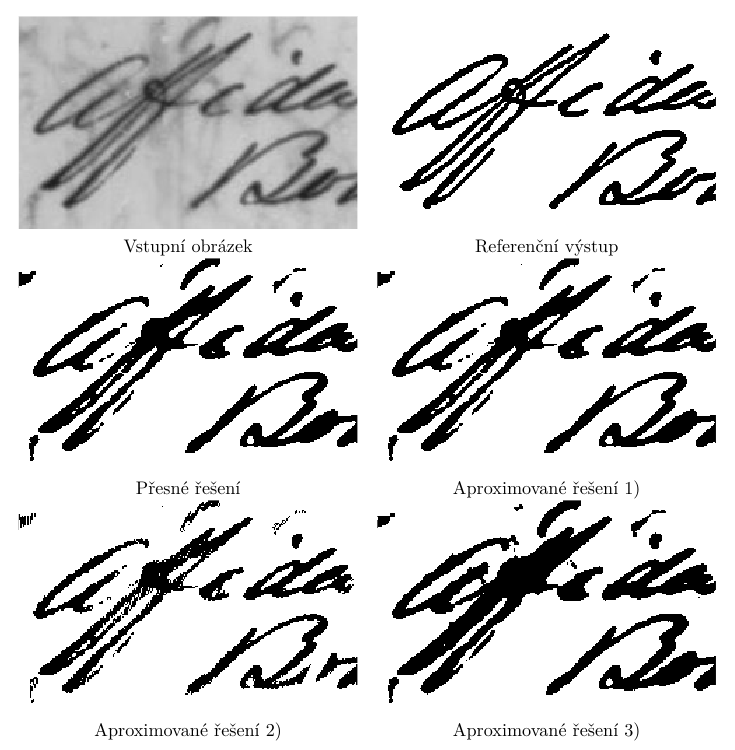
\includegraphics[width=0.9\textwidth]{obrazky-figures/approx_thresholding.png}
    \caption{Příklady výstupů aproximačních prahovacích algoritmů. Převzato z \cite{approx_image}}
    \label{fig:approx_threshold}
\end{figure}

\subsubsection{Analýza velkých dat}
Při zpracování tzv. velkých dat (angl. \textit{big data}) lze aproximovat dotazy na data, které jsou často velmi komplexní, výsledky jejich přibližných variant jsou ovšem mnohdy dostačující. Dále lze aproximovat i samotná data za účelem snížení nároků na úložný prostor. Pro nějakou třídu dotazů $Q$ na data $D$ musí platit, že pro aproximovaná data $D'$ vrátí dotazy $Q$ uspokojivé výsledky. Dotazy $Q$ bývá obvykle potřeba mírně upravit, aby vyhovovaly aproximovaným datům. V obou přístupech je třeba zvážit rovnováhu mezi efektivitou dotazů a kvalitou výsledků \cite{approx_big_data}.

\subsubsection{Strojové učení}
Přibližné počítání má ve strojovém učení (dále SU) obrovské využití, protože prostředí SU má v mnoha ohledech ideální podmínky k využítí aproximace. Mnoho úloh SU lze redukovat na problém aproximace nějaké funkce, kde daná funkce není kompletně specifikována. Samotný proces trénování modelů lze přizpůsobit tak, aby byl schopen se zotavit ze všech případných nepříznivých účinků aproximace \cite{approx_ai}.

\begin{figure}[H]
    \centering
    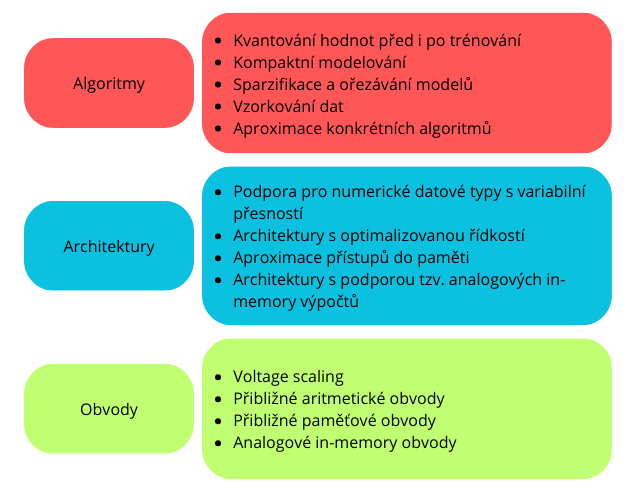
\includegraphics[width=0.7\textwidth]{obrazky-figures/ml.png}
    \caption{Přehled aproximačních technik používaných ve strojovém učení. Převzato z \cite{approx_ai}}
    \label{fig:enter-label}
\end{figure}

\subsubsection{Neaproximovatelné oblasti}
Přibližné výpočetní systémy naopak není vhodné využít tam, kde jsou z různých důvodů klíčové přesné výpočty. Typickým příkladem jsou jakékoliv peněžní transakce nebo algoritmy používané ve finančním inženýrství (angl. pojem \textit{Computational Finance}), kde by jakákoli nepřesná analýza mohla vést k velkým finančním ztrátám.

Dalším příkladem jsou tzv. bezpečnostně kritické systémy, v nichž by nepřesnosti mohly vést k ohrožení lidského života (např. systémy v automobilech, letadlech, elektrárnách apod.).

Mezi nevhodné oblasti stran aproximace lze dále řadit třeba kryptografii a šifrování, high-precision manufacturing (vysoce přesná výroba), klasické databázové systémy aj.

\section{Aproximační techniky}
V této sekci jsou stručně představeny některé používané aproximační techniky včetně uvedení jejich silných a slabých stránek a také konkrétních případů, kde je možné dané techniky využít \cite{ac_techniques}.

\subsection*{Precision scaling}
Škálování přesnosti je technika, při jejímž použití dochází ke snížení přesnosti aritmetických operací. Tuto techniku můžeme rozdělit na dva základní přístupy:
\begin{itemize}
    \item Statické škálování přesnosti -- úroveň přesnosti je stanovena na jednu předem danou hodnotu pro všechny výpočty. Tato úroveň bývá určena na základě očekávané tolerance spouštěné aplikace vůči šumu. Hlavní výhodou tohoto přístupu je jeho jednoduchost. Nevýhodou je možná nízká efektivita stran úspory energie nebo zlepšení výkonu oproti dynamickému škálování.
    \item Dynamické škálování přesnosti -- oproti statickému škálování se jedná o komplexnější techniku, při níž je úroveň přesnosti výpočtů dynamicky stanovována na základě změn tolerance spouštěné aplikace vůči šumu za běhu. Snižuje tedy přesnost výpočtů v době, kdy je tolerance vůči šumu vysoká \cite{precision_scaling}.
\end{itemize}

Obecně je tedy škálování přesnosti vhodné pro aplikace, které zpracovávají velké množství dat, která zároveň obsahují velké množství šumu.

\subsection*{Loop perforation}
Perforace smyček se zaměřuje na zrychlení provádění smyček v programu pomocí odstranění některých iterací dané smyčky. Prvním krokem při používání této techniky bývá identifikace takových smyček, jejichž zkrácením či zjednodušením nedojde k výraznému zhoršení funkčnosti programu. K tomu lze využít specializovaný kompilátor, který na základě hranice zkreslení dané uživatelem tyto smyčky identifikuje a program následně upraví \cite{code_perforation}.

Tato technika má využití v oblastech numerických výpočtů, zpracování obrazu a signálu nebo v simulacích Monte Carlo.

\begin{verbatim}
    for( i = 0; i < h; i+=4 ) { 
        /* ... */ 
    }
\end{verbatim}

\begin{verbatim}
    for( i = 0; i < h; i+=4 ) {
        if (doPerforate(i, environment)) continue;
        //...
    }
\end{verbatim}

\subsection*{Load Value Approximation}
V případě, že se procesoru nepodaří načíst data z mezipaměti (anglicky tzv. \textit{cache load miss}), je procesor nucen přistoupit k vyšším úrovním mezipaměti nebo přímo do paměti, čímž vzniká větší latence. LVA využívá aproximovatelnost některých aplikací tím, že tato data odhaduje, takže procesor může dále běžet bez větších zpoždění \cite{ac_techniques}.

Příkladem využití může být technika použitelná u grafických aplikací, kdy load-value prediktor přistupuje do paměti pouze občas (narozdíl od klasických load-value prediktorů, které přistupují do paměti při každém load miss, aby ověřily správnost své predikce). Díky tomu se výrazně sníží počet přístupů do paměti, zatímco prediktor se přesto natrénuje kvalitně \cite{load_value_approx}.

\subsection*{Memoization}
Memoizace spočívá v ukládání výstupů funkcí za účelem jejich opětovného použití při volání funkcí se stejným vstupem. Tuto metodu lze dále aproximovat znovupoužíváním těchto výstupů i u funkcí s podobným vstupem. Dochází tedy ke zrychlení díky menšímu počtu výpočtů, avšak na úkor větší paměťové náročnosti.

Memoizace je nejlépe použitelná v aplikacích, v nichž se často opakují stejné vstupy, respektive výpočty. Příkladem mohou být různé rekurzivní algoritmy, např. výpočet Fibbonaciho posloupnosti, kombinatorické vzorce nebo vyhledávací algoritmy. Přibližnou variantu memoizace lze využívat v moderních grafických aplikacích, v nichž by standardní memoizace nepřinesla významné zrychlení \cite{ac_techniques}.

\subsection*{Inexact Hardware}
Využití nepřesného hardwaru (angl. \textit{inexact hardware}) spočívá v kontrolovaném zavádění chyb do výpočetních obvodů za účelem ušetření energie, zvýšení výkonu či zmenšení plochy obvodu. Toho lze docílit např. zjednodušováním aritmetických obvodů (k tomu více v podkapitole \ref{approx_mult}).

Na obrázku \ref{fig:approx_adder} je znázorněn příklad přibližné sčítačky využívající pouze OR hradla k sečtení nejméně významných bitů \cite{log_mults}.

\begin{figure}[H]
    \centering
    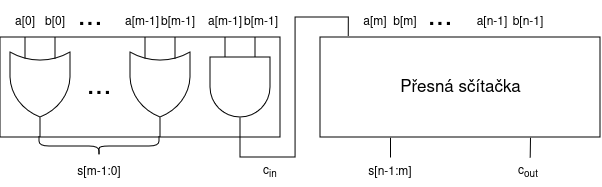
\includegraphics[width=\textwidth]{obrazky-figures/scitacka.png}
    \caption{Přibližná sčítačka lower-part-or s m nepřesnými bity. Převzato z \cite{log_mults}}
    \label{fig:approx_adder}
\end{figure}

\subsection*{Voltage Scaling}
Voltage Scaling (škálování napětí) je aproximační technika na úrovni obvodů. Jedná se o přístup, který umožňuje dynamicky měnit napětí dodávané do elektronických komponent, jako jsou mikroprocesory nebo grafické čipy, v závislosti na aktuálních požadavcích na výkon. Zvyšování napětí, tzv. \textbf{overvolting}, se používá pro zvýšení výkonu, \textbf{undervolting}, tedy snižování napětí, je využit při snaze o úsporu energie.

Při snižování napětí v obvodech mohou vznikat chyby. Například snižování napětí u paměti SRAM může vést vedle ušetření energie k častějším neúspěšným čtením a zápisům do paměti (\textit{read upset} a \textit{write failure}) \cite{ac_techniques}.

\pagebreak

\section{Hodnotící metriky} \label{error_metrics}
Jednou z klíčových otázek při implementaci aproximačních systémů je vyhodnocení míry chybovosti těchto systémů. \textbf{Chybové metriky} porovnávají výsledky přesných systémů s výsledky jejich aproximačních variant z hlediska dané metriky. Seznam některých často používaných metrik je vypsán níže \cite{circuit_library} a \cite{error_metrics}. Symbol $n_i$ v rovnicích značí počet primárních vstupů, $O_{approx}$ a $O_{orig}$ značí výstupy přibližných, respektive přesných systémů.

\bigskip

\textbf{Hammingova vzdálenost} (angl. Hamming distance, zkr. HD) mezi dvěma bitovými sekvencemi je rovna počtu pozic, na kterých se bity obou sekvencí liší \cite{hamming_dist}. Mezi používané varianty této metriky patří \textit{Průměrná Hammingova vzdálenost} nebo \textit{Maximální Hammingova vzdálenost} (v angličtině se používá výraz \textit{bit-flip error}).

Pro posuzování chybovosti násobiček není tato metoda příliš vhodná. Pokud je například očekávaný přesný výsledek výpočtu $64_{10} = 0100 0000_{2}$ a výsledek aproximace $63_{10} = 0011 1111_{2}$, jejich Hammingova vzdálenost je 7, zatímco relativní chyba je cca. $1,5 \%$.
\begin{equation}
    HD = \sum_{\forall i} OnesCount(O_{approx}^{(i)} \oplus O_{orig}^{(i)})
\end{equation}

\textbf{Pravděpodobnost chyby} (angl. error probability, zkr. EP) značí, s jakou pravděpodobností nebude výstup aproximačního systému odpovídat výstupu přesného systému.
\begin{equation}
    EP = \frac{\sum_{\forall {i:O_{approx}^{(i)} \neq O_{orig}^{(i)}}} 1} {2^{n_i}}
\end{equation}

\textbf{Průměrná absolutní chyba} (angl. mean absolute error, zkr. MAE) popisuje průměrný rozdíl mezi přesnými a přibližnými výstupy.
\begin{equation}
    MAE = \frac{\sum_{\forall i} {\left|{{O_{approx}^{(i)} - O_{orig}^{(i)}}}\right|}} {2^{n_i}}
\end{equation}

\textbf{Průměrná kvadratická chyba} (angl. mean squared error, zkr. MSE) počítá průměr druhých mocnin rozdílů mezi přesnými a přibližnými výstupy. MSE se často používá při výpočtu tzv. PSNR (zkratka z anglického \textit{Peak signal-to-noise ratio}, česky \textit{Špičkový poměr signálu k šumu}), pomocí kterého lze určovat kvalitu rekonstrukce obrázků a videí \cite{error_metrics}.
\begin{equation}
    MSE = \frac{\sum_{\forall i} {\left|{{O_{approx}^{(i)} - O_{orig}^{(i)}}}\right|^2}} {2^{n_i}}
\end{equation}

\textbf{Průměrná relativní chyba} (angl. mean relative error, zkr. MRE) uvažuje průměrnou chybu v relaci s velikostí očekávaného výstupu. Díky tomu jsou při větších hodnotách akceptovatelné větší chyby.
\begin{equation}
    MRE = \frac{\sum_{\forall i} \frac{\left|{{O_{approx}^{(i)} - O_{orig}^{(i)}}}\right|} {max(1,O_{orig}^{(i)})}} {2^{n_i}}
\end{equation}

\textbf{Nejhorší absolutní chyba} (angl. worst-case error, zkr. WCE) popisuje největší možnou chybu, které je možné při aproximaci dosáhnout.
\begin{equation}
    WCE = \max_{\forall i} \left|{O_{approx}^{(i)} - O_{orig}^{(i)}}\right|
\end{equation}

\textbf{Nejhorší relativní chyba} (angl. worst-case relative error, WCRE) uvažuje největší možnou chybu aproximačního výstupu vzhledem k očekávanému výstupu.
\begin{equation}
    WCRE = \max_{\forall i} \frac{\left|{O_{approx}^{(i)} - O_{orig}^{(i)}}\right|} {\max(1,O_{orig}^{(i)})} 
\end{equation}

\bigskip

U aproximačních obvodů jsou neméně důležité jejich \textbf{fyzické vlastnosti}. Mezi základní z nich lze zařadit zpoždění, příkon a plochu obvodu. Tyto vlastnosti je možné kombinovat v různé další složené metriky, např. PDP (z angl. \textit{Power-delay product}, tedy součin ztrát výkonu a zpoždění obvodu), ADP (z angl. \textit{Area-delay product}, tedy součin plochy a zpoždění obvodu) nebo EDP (z angl. \textit{Energy-delay product}, tedy součin zpoždění a spotřebované energie obvodu) \cite{approx_arith_circuits}.

\bigskip

Aproximační systémy je dále možné posuzovat vhodnými \textbf{kvalitativními metrikami} vzhledem k využití daného systému v konkrétní aplikaci. Mezi často používané metriky \cite{ac_techniques} patří např. výše zmíněné \textbf{PSNR}, \textbf{SSIM} (zkratka z angl. \textit{Structular similarity}, česky tedy \textit{strukturální podobnost}), \textbf{Rozdíl pixelů} (angl. \textit{Pixel difference}) nebo \textbf{UIQI} (zkratka z angl. \textit{Universal Image Quality Index}, česky tedy \textit{Univerzální index kvality obrazu}), které se používají při porovnávání podobnosti obrázků a videí.

Výstupy systémů, založených na strojovém učení nebo na shlukování, lze posuzovat např. na základě \textbf{Přesnosti} (angl. \textit{Precision}), \textbf{Výtěžnosti} (angl. \textit{Recall}), metrikou \textbf{F-score}, nebo dalších složitějších metrik \cite{clustering_eval}.

\section{Aproximační násobičky} \label{approx_mult}
Násobení je operace, která je při spouštění datově náročných aplikací (např. streamování, zpracování obrazu, strojové učení aj.) utilizována velmi často a která tím pádem spotřebuje nemalé množství energie. Mnohé z těchto aplikací jsou ovšem schopné vytvořit dostatečně dobrý výsledek i přes nepřesnosti v násobení. Dalším příkladem využití přibližných násobiček jsou zařízení z oblasti internetu věcí, u nichž je kladen důraz na co nejmenší spotřebu energie a u nichž také mnohdy není nutné vše počítat přesně \cite{approx_mult_survey}.

Tato podkapitola se zaměřuje nejprve na vysvětlení funkcionality binárních násobiček a následně na popis základních přístupů k vytváření přibližných násobiček.

\subsubsection{Základní princip binárních násobiček}
Při binárním násobení uvažujeme pouze 2 hodnoty -- 1 a 0. Z toho důvodu je možné na binární násobení nahlížet jako na sekvenci sčítání a bitových posunů. Uvažme příklad z obrázku \ref{fig:binmult}, kde vstup $x$ je násoben vstupem $y$. Operaci násobení lze rozdělit do 3 fází: načtení dat na vstupu, generování částečných součinů a finální součet.

Základní binární násobička funguje tak, že se postupně roznásobují jednotlivé bity vstupu $y$ se všemi bity vstupu $x$ a následně na základě váhy bitu $y$ dochází k bitovému posunu vlevo. První řádek částečných součinů v příkladu z obrázku \ref{fig:binmult} tedy vznikne roznásobením bitu $y_0$ se všemi bity vstupu $x$, atd. Nakonec se všechny částečné součiny sečtou v konečný výsledek.

\begin{figure}[H]
    \centering
    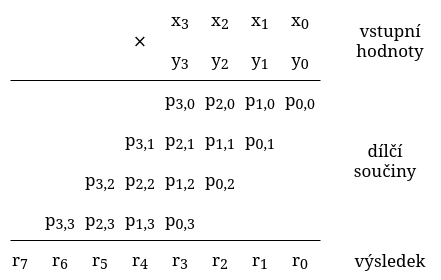
\includegraphics[width=0.55\textwidth]{obrazky-figures/binmult.png}
    \caption{Binární násobička 4x4 bity}
    \label{fig:binmult}
\end{figure}

Násobení jednotlivých bitů je implementováno jednoduše pomocí hradel AND, kritickou sekcí procesu násobení je propagace přenosu (angl. \textit{carry}) z nižšího bitu na vyšší bit. Přístupů k řešení tohoto problému je mnoho, jedním z nich je například tzv. ripple-carry sčítačka, kde se přenosy propagují postupně zprava doleva, nebo také tzv. carry-save sčítačka, kde se přenosy propagují diagonálně za účelem zrychlení výpočtu \cite{approx_mult_survey}.

\begin{figure}[H]
    \centering
    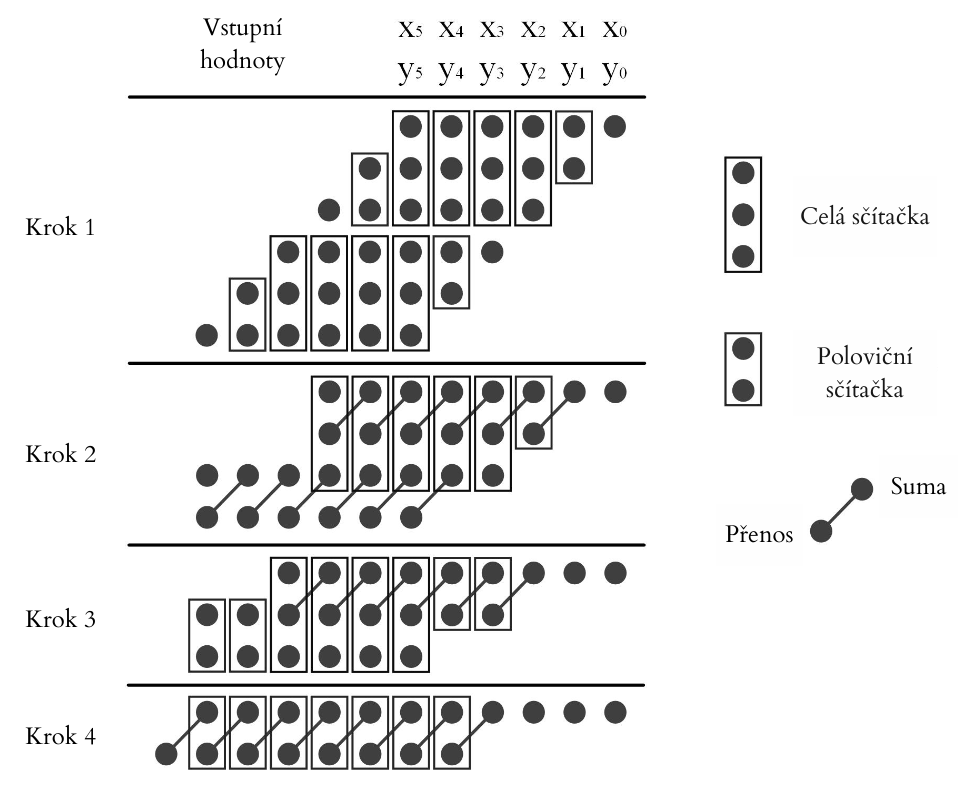
\includegraphics[width=0.75\textwidth]{obrazky-figures/wallacetree.png}
    \caption{Příklad Wallace-Tree násobičky. Převzato z \cite{approx_mult_survey}}
    \label{fig:wallacetree}
\end{figure}

Další zrychlení přináší princip tzv. Wallace Tree, v rámci něhož se seskupují 3 částečné součiny po sloupcích, které generují 2 výstupy -- sumu a přenos. Tato operace se opakuje, dokud nezůstanou poslední dva řádky částečných součinů, které se poté sečtou v konečný výsledek. V této násobičce jsou využívány úplné a částečné sčítačky, dalšího zrychlení lze docílit utilizací paralelních výpočtů \cite{wallace_tree}. Ilustrace této násobičky je na obrázku \ref{fig:wallacetree}.

\subsubsection{Aproximace vstupních hodnot}
Jednoduchým a přesto efektivním způsobem aproximace je aproximace vstupních dat. Toho lze docílit např. uříznutím několika nejméně významných bitů (zkr. LSB z angl. \textit{least significant bit}), což má menší vliv na celkový výsledek výpočtu, než uříznutí několika nejvíce významných bitů (zkr. MSB z angl. \textit{most significant bit}) \cite{approx_mult_survey}. 

Existují dvě základní metody segmentace dat -- dynamická a statická. Dynamická segmentace dat (DSM) spočívá v detekci prvního nenulového bitu a oříznutí následujících $k$ bitů. Při statické segmentaci dat (SSM) dochází k volbě jedné z předem daných strategií. Na obrázku \ref{fig:dsm_ssm} jsou ilustrovány obě metody. U SSM jsou v tomto případě následující možnosti: $k$ nejméně významných bitů, $k$ nejvíce významných bitů nebo $k$ prostředních bitů jako kompromis.

SSM zpravidla potřebuje méně hardwarových zdrojů než DSM, na druhou stranu její výsledek bývá méně efektivní, protože může obsahovat některé redundantní bity (např. nulové MSB).

\begin{figure}[H]
    \centering
    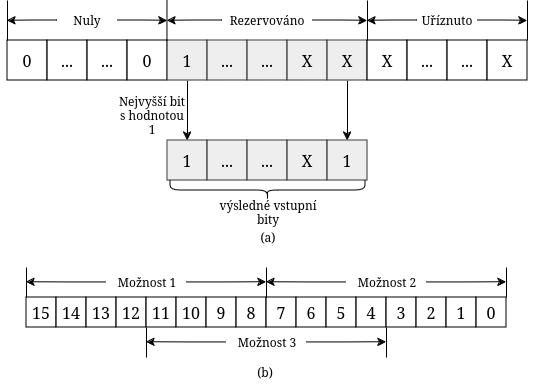
\includegraphics[width=0.8\textwidth]{obrazky-figures/dsm_ssm.png}
    \caption{(a) Příklad oříznutí DSM; (b) Příklad oříznutí SSM. Převzato z \cite{approx_mult_survey}}
    \label{fig:dsm_ssm}
\end{figure}

\subsubsection{Aproximace při generování částečných součinů}
Jedním z možných přístupů je využití malých bloků nepřesných násobiček k vytvoření dílčích součinů a poté sečtení těchto různě bitově posunutých dílčích součinů. Takové násobičky lze nazývat pojmem \textit{Nedostatečně navržená násobička} neboli anglicky \textbf{Under-designed multiplier}. 

Příkladem stavebního bloku může být násobička na obrázku \ref{fig:approx_acc_mult}. Jak lze pozorovat v Karnaughově mapě v tabulce \ref{tab:kmap2x2}, tato násobička je přesná pro 15 ze 16 možných vstupních kombinací (nepřesný výsledek je v tabulce vyznačen červeně). Změna oproti přesné násobičce je v tom, že výsledek vstupu $3\cdot3$ je reprezentován bity $111$ oproti přesnému výsledku $1001$, díky čemuž se snížila plocha obvodu téměř na polovinu (5 logických hradel oproti 9 u přesné násobičky, méně drátů) s pravděpodobností chyby pouze $\frac{1}{16}$ \cite{underdesigned_mult}.

\begin{figure}[H]
    \centering
    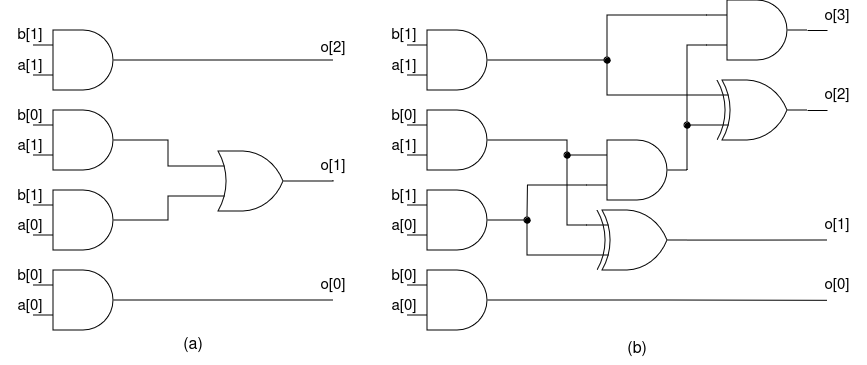
\includegraphics[width=\textwidth]{obrazky-figures/approx_acc_mult.png}
    \caption{(a) Přibližná násobička 2x2 bity (b) Přesná násobička 2x2 bity}
    \label{fig:approx_acc_mult}
\end{figure}

\begin{table}[H]
\centering
\begin{tabular}{|
>{\columncolor[HTML]{FFFFFF}}l |
>{\columncolor[HTML]{FFFFFF}}l |
>{\columncolor[HTML]{FFFFFF}}l |
>{\columncolor[HTML]{FFFFFF}}l |
>{\columncolor[HTML]{FFFFFF}}l |}
\hline
 $\times$  & 00  & 01  & 11                         & 10  \\ \hline
00 & 000 & 000 & 000                        & 000 \\ \hline
01 & 000 & 001 & 011                        & 010 \\ \hline
11 & 000 & 011 & {\color[HTML]{FE0000} 111} & 110 \\ \hline
10 & 000 & 010 & 110                        & 100 \\ \hline
\end{tabular}
\caption{Karnaughova mapa pro nepřesnou násobičku z obrázku \ref{fig:approx_acc_mult}}
\label{tab:kmap2x2}
\end{table}

Na obrázku \ref{fig:larger_mults} je znázorněn příklad násobičky 4x4 bitů složené ze 4 bloků násobiček 2x2
bity. A a X jsou vstupní hodnoty, dolní indexy H, respektive L značí 2 vyšší, respektive 2 nižší bity vstupu. V jednotlivých blocích postupně dochází k roznásobení všech kombinací dvojic vstupních bitů. Tyto dílčí výsledky jsou následně bitově posunuty a sečteny, čímž vzniká celkový výsledek násobení.

\begin{figure}[H]
    \centering
    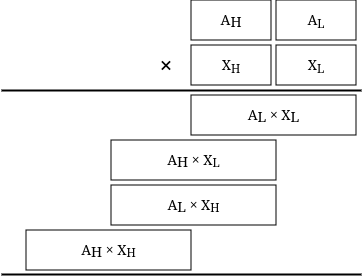
\includegraphics[width=0.5\textwidth]{obrazky-figures/larger_mults.png}
    \caption{Tvorba násobiček z menších bloků. Převzato z \cite{underdesigned_mult}}
    \label{fig:larger_mults}
\end{figure}

\subsubsection{Aproximace při závěrečném sčítání}
Pro závěrečné sčítání částečných součinů se používají sčítačky a kompresory, proto je přirozené uvažovat o aproximaci těchto komponent za účelem aproximace celé násobičky. Přístupů k tomuto řešení existuje celá řada, v posledních letech výzkumníci pracují s myšlenkou rozdělení matice částečných součinů na několik skupin (obvykle 2 nebo 3), přičemž u každé skupiny by docházelo k jinak velké aproximaci. U příkladu na obrázku \ref{fig:accumulation_approx} by nejvíce významné bity zůstaly nezměněny, prostřední bity by podléhaly určité aproximaci a nejméně významné bity by byly uříznuty nebo akumulovány pouze pomocí OR hradel.

\begin{figure}[H]
    \centering
    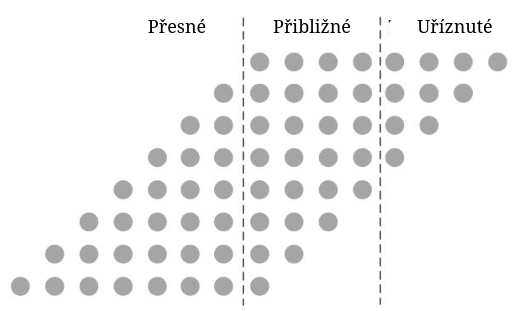
\includegraphics[width=0.6\textwidth]{obrazky-figures/accumulation_approx.png}
    \caption{Příklad rozdělení matice částečných součinů na skupiny s různou úrovní aproximace. Převzato z \cite{approx_mult_survey}}
    \label{fig:accumulation_approx}
\end{figure}

Další možností je rozdělení matice částečných součinů pomocí vertikálního a horizontálního uříznutí. Jak je vidět v příkladu na obrázku \ref{fig:bam}, všechny částečné součiny nahoru od horizontální hranice jsou při konečném součtu ignorovány. To stejné platí i pro částečné součiny napravo od vertikální hranice. Pomocí posouvání těchto hranic lze modifikovat míru aproximace. Takto navržené násobičky se nazývají anglickým pojmem \textbf{Broken-Array Multiplier}, tedy násobička s rozbitou maticí částečných součinů \cite{bio_inspired_blocks}. 

\begin{figure}[H]
    \centering
    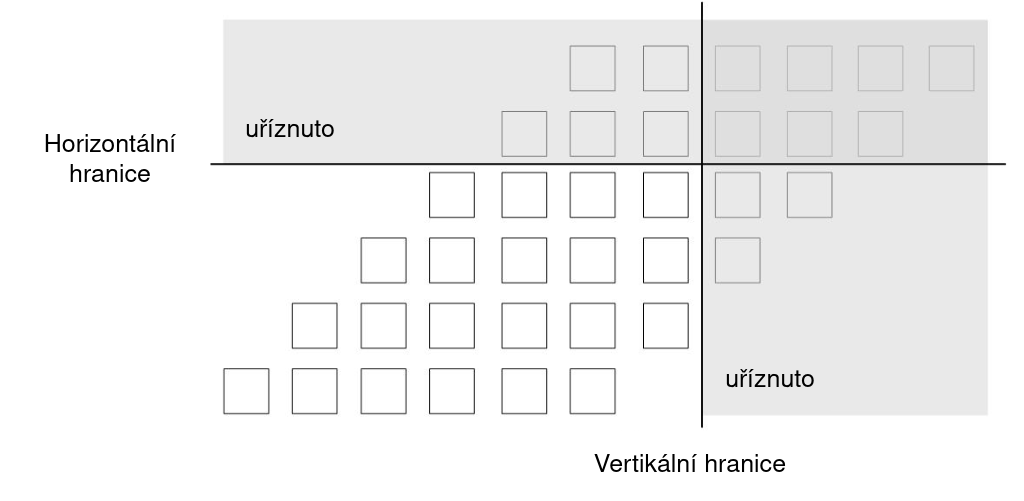
\includegraphics[width=0.85\textwidth]{obrazky-figures/bam.png}
    \caption{Příklad násobičky typu Broken-Array. Převzato z \cite{bio_inspired_blocks}}
    \label{fig:bam}
\end{figure}

\subsubsection{Logaritmické násobičky}
Násobičky lze aproximovat také na úrovni algoritmů. Jednou z možností je tvorba logaritmických násobiček, kde lze na násobení nahlížet jako na součet logaritmů obou činitelů. Při násobení čísel $A \cdot B$ lze logaritmus pro číslo $A$ vyjádřit následovně \cite{mitchell_log}:

\begin{equation}
    A = 2^{k_1}(1+x_1),
\end{equation}

\begin{equation}
    \log_2(A) = k_1 + \log_2(1+x_1),
\end{equation}

kde $A$ je činitel, $k_1$ je pozice nejvýznamnějšího bitu s hodnotou 1 a $x_1$ je desetinná část ležící v intervalu $\langle0,1)$. Stejnou formulí s parametry $k_2$ a $x_2$ lze vyjádřit i logaritmus pro činitel $B$. Logaritmus samotného násobení lze poté vyjádřit následujícím způsobem:

\begin{equation}
    \log_2(A \cdot B) = k_1 + k_2 + log_2(1+x_1) + log_2(1 + x_2)
\end{equation}

Implementace tohoto výpočtu vyžaduje použití detektoru nejvyššího jedničkového bitu (angl. \textit{Leading-one detector}), binárně-logaritmických převodníků (angl. \textit{logarithm-binary converter} a \textit{binary-logaritm converter}) a sčítačky \cite{approx_mult_survey}. Pro snížení implementační náročnosti lze výpočet aproximovat následovně:

\begin{equation}
    \log_2(x+1) \approx x, 0 \leq x < 1.
\end{equation}

Tím vzniká rovnice $A \cdot B \approx 2^{k_1+k_2+x_1+x_2} = 2^{k_1+k_2} \cdot 2^{x_1+x_2}$. Na základě přenosu z výpočtu $x_1 + x_2$ může být výpočet $A \cdot B$ dále aproximován jako:

\begin{equation}
    A \cdot B \approx \Bigg\{ 
    \begin{array}{ll}
        2^{k_1+k_2}(x_1+x_2+1) & \text{pro } x_1 + x_2 < 1, \\
        2^{k_1+k_2+1}(x_1+x_2) & \text{pro } x_1 + x_2 \geq 1.
    \end{array}
\end{equation}

Při porovnání s výsledkem přesného násobení (za předpokladu, že $x_1 + x_2 < 1$) lze chybu aproximovaného výpočtu vyjádřit jako \cite{approx_mult_survey}:

\begin{equation}
    \begin{array}{rl}
       Chyba & = A \cdot B - 2^{k_1+k_2}(x_1+x_2+1) \\
             & = 2^{k_1+k_2}(1+x_1)(1+x_2)-2^{k_1+k_2}(x_1+x_2+1) \\
             & = 2^{k_1+k_2}x_1x_2
    \end{array}
\end{equation}

\chapter{Statistické ověřování modelů}
\label{smc}
Chyby v počítačových systémech mohou mít v dnešní době drastické dopady na společnost, včetně ohrožení lidských životů, proto je dokazování správnosti těchto systémů mimořádně důležitá činnost. K verifikaci počítačových systémů tradičně existují dva základní přístupy: statická a dynamická analýza (viz obrázek \ref{fig:verifikace_rozdeleni}).

Statická analýza využívá metody formální verifikace, např. ověřování modelů, kterými lze garantovat (matematicky dokázat) bezchybnost nějakého systému. Oproti tomu dynamická analýza spočívá v simulování a testování daného systému, přičemž chyby se zachytávají při bězích jednotlivých testovacích případů. Ideální by bylo všechny systémy formálně verifikovat a zamezit tak možnosti výskytu chyby, na formální verifikaci mnohých reálných komplexních systémů ovšem nestačí výpočetní výkon současných počítačů. Tyto systémy lze ověřovat testováním, které ale pro změnu téměř nikdy neodhalí všechny chyby systému.

\begin{figure}[H]
    \centering
    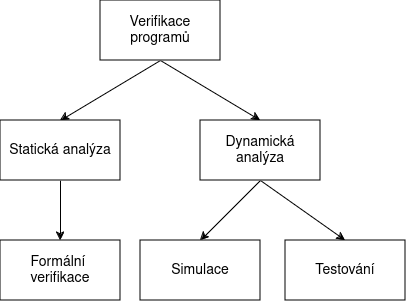
\includegraphics[width=0.6\textwidth]{obrazky-figures/verifikace_rozdeleni.png}
    \caption{Rozdělení přístupů k verifikaci programů}
    \label{fig:verifikace_rozdeleni}
\end{figure}

Metody formální verifikace se původně zaměřovaly na diskrétní chování systémů. Výzkum v posledních letech ovšem ukazuje, že spojitý (reálný) čas hraje u mnohých systémů klíčovou roli, a měl by proto být zohledněn při verifikaci. K modelování takových systémů proto vznikly časové automaty. Jedním z nejvýznamnějších nástrojů, které se prací s časovými automaty zabývají, je UPPAAL \cite{uppaal_smc}.

Časové automaty ovšem nejsou dostatečně expresivní na to, aby dokázaly popsat chování komplexnějších systémů s reálným časem. Chování těchto systémů často závisí na stochastických jevech, ověřování modelů takových systémů je nerozhodnutelné. S alternativním řešením tohoto problému přichází rozšíření UPPAAL SMC, které tyto systémy reprezentuje pomocí sítí stochastických časových automatů, jejichž chování může záviset na stochastických a nelineárních dynamických jevech. K efektivní analýze vlastností modelů využívá \textbf{statistického ověřování modelů}.

Zdrojem následujících 3 odstavců je primárně článek \cite{automata_zoo}. Stochastické časové automaty jsou součástí hierarchie výpočetních modelů založených na automatech, která je znázorněna ve stromě na obrázku \ref{fig:automata_zoo}. Modely, které jsou umístěné ve stromě výše, dědí vlastnosti od svých níže postavených předchůdců a obvykle přidávají některé funkcionality navíc.

Jak z obrázku plyne, většina těchto výpočetních modelů vychází z označených přechodových systémů, které zavádí nedeterministický výběr přechodu a také je možné pomocí nich modelovat paralelní systémy umožňující komunikaci mezi jednotlivými modely \cite{mc_principles}. Diskrétní pravděpodobnostní rozhodování má zase původ v Markovových řetězcích s diskrétním časem. Kombinací těchto dvou vlastností vznikají Markovovy rozhodovací procesy. 

Časové automaty zavádějí modelování reálného času, v kombinaci s diskrétním pravděpodobnostním rozhodováním poté vznikají pravděpodobnostní časové automaty. Stochastické časové automaty k těmto vlastnostem přidávají možnost pracovat se spojitým pravděpodobnostním rozdělením. Kombinací s hybridními automaty, které zavádějí spojitou dynamiku umožňující modelovat složité fyzikální procesy, vznikají stochastické hybridní automaty.

\begin{figure}[H]
    \centering
    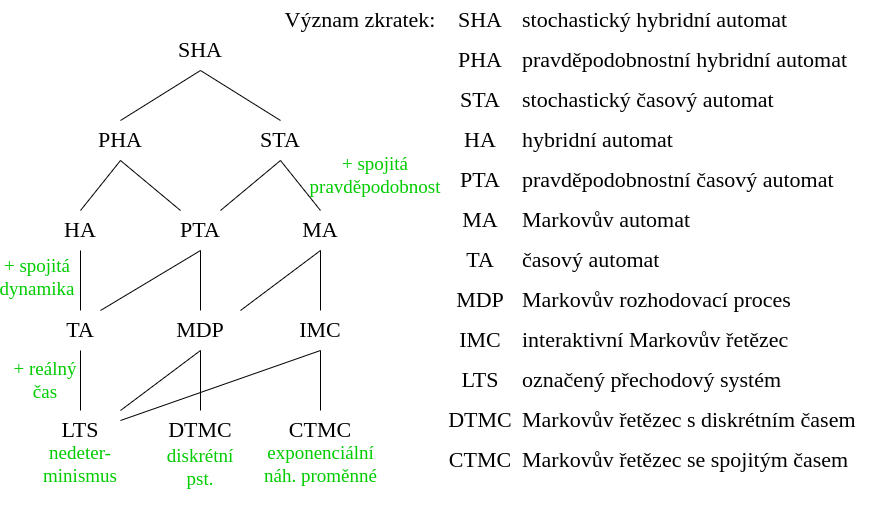
\includegraphics[width=\textwidth]{obrazky-figures/automata_zoo.png}
    \caption{Hierarchie kvantitativních automatů, převzato z \cite{automata_zoo}}
    \label{fig:automata_zoo}
\end{figure}

Tato kapitola se zabývá nejprve uvedením principu statistického ověřování modelů, poté definicí časových automatů a nakonec rozborem nástroje UPPAAL včetně jeho uživatelského rozhraní, dotazovacího jazyka a dalších rozšíření.

\pagebreak

\section{Ověřování modelů}
Tato kapitola čerpá z publikace \cite{mc_principles}.

Ověřování modelů (angl. \textit{Model Checking}) je jeden z možných přístupů verifikace počítačových systémů. \textbf{Verifikace systému} spočívá ve snaze zajistit, že daný zkoumaný systém splňuje určité vlastnosti. Vlastnosti, které by měl daný systém splňovat, vyplývají ze \textbf{specifikace systému}. V rámci takové specifikace je definováno očekávané chování systému. Záváda systému je objevena v takový okamžik, kdy není splněna některá z požadovaných vlastností systému. \textbf{Správnost systému} je vždy relativní vzhledem ke specifikaci, nejedná se o absolutní vlastnost systému jako takového.

Verifikace jako součást vývoje software je znázorněna v rámci tzv. V-modelu na obrázku \ref{fig:vmodel}. Jak je vidět, prvním krokem vývoje systému je analýza požadavků zákazníka. Následují návrhy různých vrstev systému a vznikají první prototypy. Poté dochází k verifikaci jednotlivých částí systému, ať už pomocí ověřování modelů, testování či jiných metod. Neméně důležitá je \textbf{validace systému}, při níž je ověřováno, že systém skutečně splňuje požadavky dané zákazníkem.

\begin{figure}[H]
    \centering
    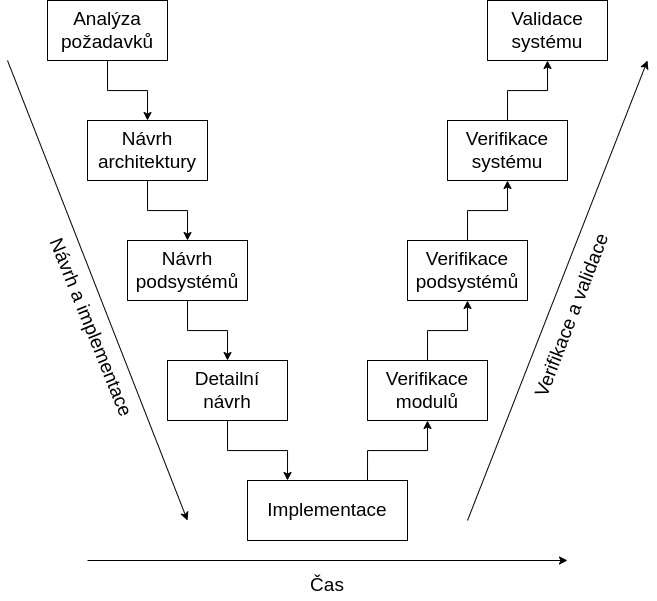
\includegraphics[width=0.8\textwidth]{obrazky-figures/vmodel.png}
    \caption{V-model popisující fáze vývoje počítačového systému}
    \label{fig:vmodel}
\end{figure}

Ověřování modelů je technika, v rámci níž dochází k procházení kompletního stavového prostoru zkoumaného modelu. Díky tomu je možné s jistotou tvrdit, že model splňuje či nesplňuje danou vlastnost. Ze skutečnosti, že je procházen celý stavový prostor, vyplývá i největší nevýhoda ověřování modelů -- pro složité systémy s velkým počtem stavů může být klasické ověřování modelů příliš výpočetně a paměťově náročné.

Proces ověřování modelů je ilustrován na obrázku \ref{fig:mc_scheme}.

Ve \textbf{fázi modelování} dochází nejprve k vytvoření modelu systému v daném modelovacím jazyce. Ke zběžnému zhodnocení vytvořeného modelu je vhodné provést několik simulací. Také je potřeba formalizovat požadavky na systém v rámci jazyka určeného pro specifikaci vlastností.

Ve \textbf{fázi běhu} dochází ke spouštění programu pro ověřování modelů nad jednotlivými dotazy za účelem ověření formalizovaných požadavků.

Ve \textbf{fázi analýzy} jsou vyhodnocovány výsledky jednotlivých ověřovacích dotazů. V případě, že zkoumaná vlastnost nebyla splněna, dojde k vygenerování tzv. \textbf{protipříkladu}. Protipříklad je vygenerovaná stopa (průchod jednotlivých stavů systému), která demonstruje porušení zkoumané vlastnosti.

Jakmile jsou všechny vlastnosti ověřeny a splněny, lze modelovaný systém označit za správný.

\begin{figure}[H]
    \centering
    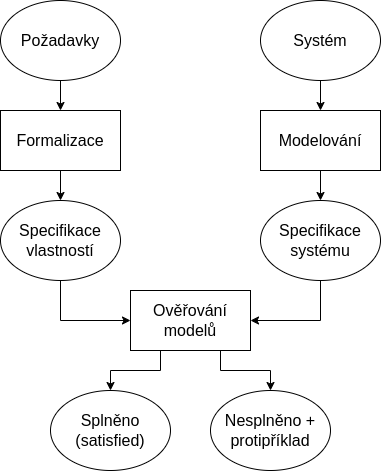
\includegraphics[width=0.5\textwidth]{obrazky-figures/model_checking_scheme.png}
    \caption{Schéma principu ověřování modelů, převzato z \cite{quantitative_analysis}}
    \label{fig:mc_scheme}
\end{figure}

\subsection{Alternativní verifikační techniky}
V této podsekci jsou stručně představeny některé další techniky verifikace počítačových systémů.

\subsubsection{Verifikace software}
\begin{itemize}
    \item Testování -- spočívá v opakovaném spouštění programů (jak celých výsledných programů, tak jejich částí) s různými vstupními parametry a různými vnějšími podmínkami za účelem objevení možných chyb v systému.
    \item Peer Review (vzájemné hodnocení) -- kontrola zdrojových kódů prováděna týmem softwarových inženýrů, který se v nejlepším případě nepodílel na vývoji daného softwaru. Při těchto kontrolách nedochází k překladu kódu ani ke spouštění výsledné aplikace, kód je analyzován staticky.
\end{itemize}

\subsubsection{Verifikace hardware}
\begin{itemize}
    \item Emulace -- jedná se o druh testování, při němž je nějaký rekonfigurovatelný obecný hardwarový systém (emulátor) nastaven tak, že jeho vlastnosti odpovídají vlastnostem zkoumaného systému. Poté je podrobován testům s různými vstupními parametry.
    \item Simulace -- v případě simulací je model daného obvodu zkonstruován a poté jsou na něm prováděny simulace. Modely obvodů jsou obvykle napsány v jazycích určených pro popis hardwaru (\textit{hardware description language}), jako jsou např. Verilog nebo VHDL.
    \item Strukturální analýza -- kombinuje různé ověřovací techniky, jako např. syntézu (\textit{Synthesis}), časovou analýzu (\textit{Timing Analysis}) nebo kontrolu ekvivalence (\textit{Equivalence checking}).
\end{itemize}

\section{Úvod do statistického ověřování modelů}
Tato sekce čerpá z článku \cite{uppaal_smc}. 

Statistické ověřování modelů (SMC) představuje určitý kompromis mezi testováním a klasickými formálními technikami ověřování modelů. Jedná se o techniku, která spočívá v monitorování simulací nějakého systému se zaměřením na určité vlastnosti a poté využití výsledků simulací k získání statistik sloužících k odhadu správnosti daného systému. Mezi používané statistické metody se řadí sekvenční testování hypotéz (\textit{sequential hypothesis testing}) nebo simulace Monte Carlo.

SMC nachází využití u systémů, které jsou příliš komplikované pro tradiční metody ověřování modelů z důvodu exploze stavového prostoru. Konkrétně se SMC využívá při ověřování systémů v biologii \cite{smc_biology}, systémů zaměřujících se na optimalizaci spotřeby energie \cite{smc_energy_centric}, v leteckém a automobilovém průmyslu i jinde. Důvodem tohoto úspěchu je relativně jednoduchá implementace a snadné pochopení a používání i pro uživatele, kteří nejsou výzkumníky v oblasti simulací a ověřování modelů. Využití statistiky také umožňuje aproximovat řešení jinak nerozhodnutelných problémů.

Mezi hlavní výhody statistického ověřování modelů lze zařadit:
\begin{itemize}
    \item Škálovatelnost -- díky tomu, že SMC neprochází celý stavový prostor, je možné ověřovat i systémy s velmi velkým až nekonečným stavovým prostorem.
    \item Efektivnost -- je výpočetně efektivnější pro systémy se složitým a stochastickým chováním, protože využívá spíše statistické odvozování oproti symbolickým výpočtům.
    \item Flexibilita -- SMC může být aplikováno na celou řadu diskrétních, spojitých i hybridních systémů.
\end{itemize}

Statistické ověřování modelů má přes své nesporné výhody i několik omezení. Přesnost výsledků závisí jak na počtu simulací, tak na správné formě dotazu a také využití správné statistické metody. Jevy, které se v chování systému objevují pouze vzácně, nemusejí být při nízkém počtu simulací objeveny a zohledněny při odvozování výsledků.

\section{Časové automaty}
Celá tato sekce čerpá z publikace \cite{mc_principles}. 

Časové automaty modelují chování \textbf{časově kritických systémů} (angl. \textit{time-critical system}). To jsou takové systémy, jejichž správná funkčnost nezávisí pouze na logickém výsledku nějakého výpočtu, ale také na čase, ve kterém daný výsledek vznikl. Může se jednat o ovladače zařízení v počítačích, různé komunikační protokoly a obecně systémy, které musí na něco reagovat v rámci určitého časového úseku. Díky zavedení časových omezení do automatů lze poté modelovat tvrzení jako např. \uv{Semafor se přepne na zelenou v rámci následujících 30 sekund.} Čas lze v rámci časových automatů uvažovat jak diskrétní, tak spojitý.

Časové automaty tedy zavádějí časové proměnné neboli hodiny, které se liší od běžných proměnných tím, že lze pouze sledovat jejich hodnotu nebo je resetovat na 0 (tedy nelze je nastavit na libovolnou hodnotu). Omezení, která jsou závislá na čase (tedy na hodnotách hodin), lze nazývat časovými omezeními (v angličtině \textbf{clock constraints}). Každé takové omezení odpovídá gramatice

\begin{equation*}
    g ::= x < c \hspace{0.15cm} \Big| \hspace{0.15cm} x \leq c \hspace{0.15cm} \Big| \hspace{0.15cm} x > c \hspace{0.15cm} \Big| \hspace{0.15cm} x \geq c \hspace{0.15cm} \Big| \hspace{0.15cm} g \wedge g,
\end{equation*}

kde $c \in \mathbb{N}$ a $x$ je proměnná z množiny hodin. Časová omezení, která neobsahují konjunkce, jsou atomická.

Časová omezení lze přiřazovat jak k lokacím, tak k hranám automatů, v obou případech se jejich význam liší. Časová omezení u lokací se nazývají pojmem \textbf{invariant} a značí maximální dobu, kterou může automat v dané lokaci strávit. Časovým omezením u hran se říká strážci (angl. \textbf{guard}). Ta udávají, po jaké době je možné učinit přechod po dané hraně do další lokace (tedy jak dlouho minimálně musí automat strávit v lokaci, z níž hrana vychází).

\bigskip

Časový automat je uspořádaná osmice $TA = (Loc, Act, C, \hookrightarrow, Loc_0, Inv, AP, L)$, kde

\begin{itemize}
    \item $Loc$ je konečná množina lokací,
    \item $Loc_0 \subseteq Loc$ je množina počátečních lokací,
    \item $Act$ je konečná množina akcí,
    \item $C$ je konečná množina hodin,
    \item $\hookrightarrow \hspace{0.15cm} \subseteq Loc \times CC(C) \times Act \times 2^C \times Loc$ je relace přechodu,
    \item $Inv: Loc \rightarrow CC(C)$ je funkce přiřazení invariantu (\textit{invariant-assignment function}),
    \item $AP$ je konečná množina atomických tvrzení (\textit{atomic proposition}),
    \item $L: Loc \rightarrow 2^{AP}$ je funkce označení (názvů) lokací.
\end{itemize}

Intuitivní reprezentace přechodu $\ell \xhookrightarrow{g:\alpha,D} \ell'$, kde $g$ je časové omezení, $\alpha$ je akce a $D$ je množina hodin, je následující: Automat přechází z lokace $\ell$ do lokace $\ell'$ pokud je splněno časové omezení $g$. Dále je provedena akce $\alpha$ a všechny hodiny z množiny $D$ jsou resetovány na hodnotu 0. Příklad znázornění jednoduchého časového automatu je možné vidět v následující sekci na obrázku \ref{fig:lamp}.

\subsection{Stochastické časové automaty} \label{stochastic_ta}
Tato podsekce čerpá z článku \cite{uppaal_smc}.

Stochastické časové automaty (STA z angl. \textit{stochastic timed automata}) rozšiřují klasické časové automaty o pravděpodobnostní rozhodování. Oproti klasickým časovým automatům, u nichž je rozhodování o přechodu do další lokace nedeterministické, dochází u STA k rozhodování dle pravděpodobnostních rozdělení, která mohou či nemusí být dána uživatelem.

Podobně nedeterministické rozhodování o zpoždění času je obohaceno o pravděpodobnostní rozdělení. U ohraničených zpoždění se jedná o uniformní rozdělení, u neohraničených zpoždění poté o exponenciální rozdělení.

Na obrázku \ref{fig:sta_examples} jsou vidět 3 příklady stochastických časových automatů. Jak vyplývá z časových omezení u lokací a hran jednotlivých automatů, dosažitelnost stavu \texttt{END} se pohybuje v intervalech (a) $\langle 6, 12 \rangle$, (b) $\langle 4, 12 \rangle$, resp. (c) $\langle 0, \infty )$. Pravděpodobnostní rozdělení dosažitelnosti lokace \texttt{END} pro jednotlivé automaty lze pozorovat na obrázku \ref{fig:sta_reachability}. U automatů $A_1$ a $A_2$ se jedná o sečtení rovnoměrných rozdělení časových omezení jejich jednotlivých přechodů. Automat $A_3$ neobsahuje žádná časová omezení, proto je zpoždění v jednotlivých lokacích dáno exponenciálním rozdělením, v tomto případě s rychlostí danou uživatelem (hodnoty $\frac{1}{2}$, $2$, $\frac{1}{4}$).

U automatů $A_2$ a $A_3$ je také možné pozorovat větvení (tzv. \textit{branch point}), v obou případech hned za počáteční lokací. V těchto větvících bodech je možné definovat, s jakou pravděpodobností se provede přechod do jedné z následujících lokací. Např. u automatu $A_2$ se jedná o hodnoty 1 a 5, tedy do horní části se automat dostane s pravděpodobností $\frac{1}{6}$, do spodní pak s pravděpodobností $\frac{5}{6}$.

\begin{figure}[H]
  \begin{minipage}[b]{.49\linewidth}
    \centering
    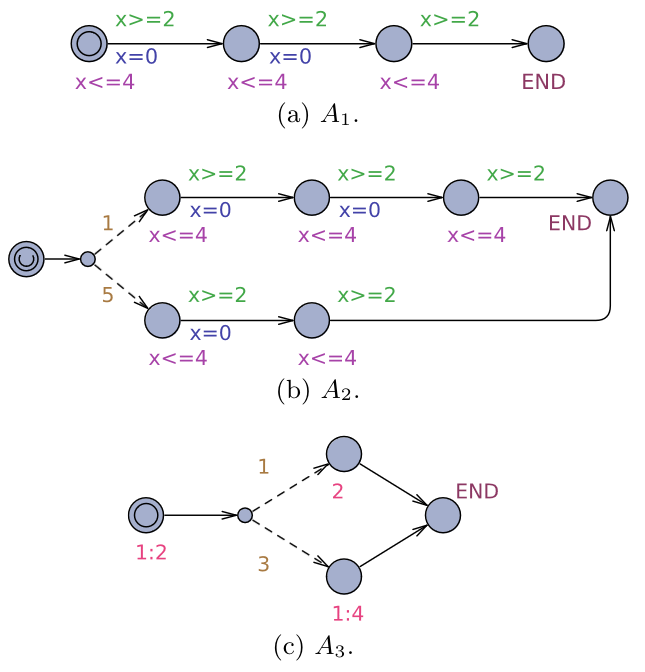
\includegraphics[width=\linewidth]{obrazky-figures/sta_examples.png}
    \caption{Příklady stochastických časových automatů, převzato z \cite{uppaal_smc}}
    \label{fig:sta_examples}
  \end{minipage}
  \begin{minipage}[b]{.49\linewidth}
    \centering
    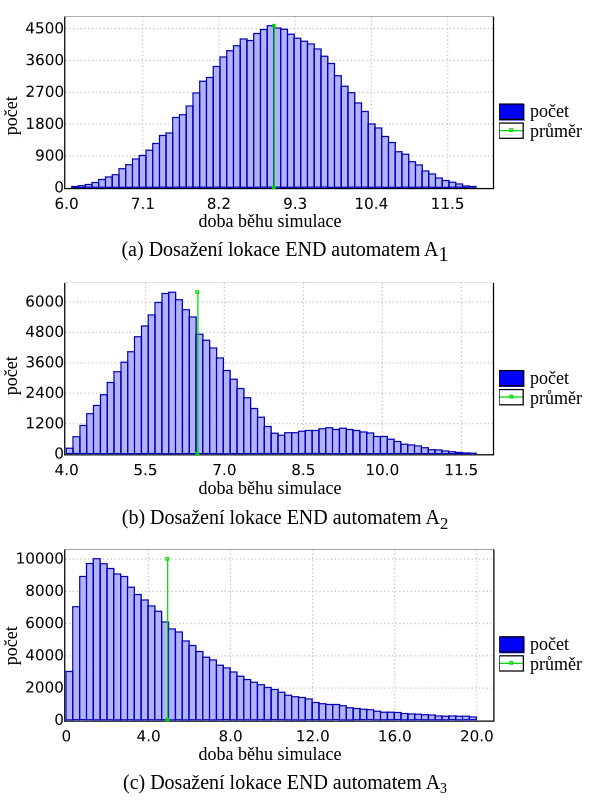
\includegraphics[width=\linewidth]{obrazky-figures/sta_reachability.png}
    \caption{Rozdělení dosažitelnosti lokace END, převzato z \cite{uppaal_smc}}
    \label{fig:sta_reachability}
  \end{minipage}\hfill
\end{figure}

\section{Modelovací nástroj UPPAAL} \label{uppaal}
UPPAAL je program určený k modelování, simulaci a verifikaci systémů s realným časem. Byl vyvinut za spolupráce výzkumníků z univerzit Aalborg (Dánsko) a Uppsala (Švédsko). První vydání vzniklo v roce 1995, v době vzniku této bakalářské práce byla aktuální verze 5.0 vydaná v červnu 2023. Uživatelské rozhraní je napsáno v jazyce Java, zbytek v C++. Na C++ je také postaven jazyk používaný k deklaracím a definicím součástí modelů (k tomu více níže).

Kromě rozšíření UPPAAL SMC využívaného v této práci UPPAAL nabízí rozšíření UPPAAL Stratego zaměřující se na strategie her, UPPAAL Tiga využivající časových herních modelů (\textit{timed game automata}) k řešení her, UPPAAL CORA (zkratka z angl. \textit{Cost Optimal Reachability Analysis}) zabývající se efektivní analýzou dosažitelnosti modelů a UPPAAL TRON sloužící k tzv. black-box testování systémů s reálným časem.

\subsection{Rozšíření časových automatů v nástroji UPPAAL}
Modelovací jazyk programu UPPAAL rozšiřuje časové automaty o následující součásti \cite{uppaal_intro}:

\begin{itemize}
    \item Šablony (Templates) -- při definici automatů je možné specifikovat parametry libovolného validního datového typu, které se automatu předají jako argumenty při inicializaci.
    \item Konstanty -- konstantní datové proměnné, pouze integer. Deklarovány jako \texttt{const name value}.
    \item Ohraničené proměnné -- proměnné deklarované jako \texttt{int[min, max] name}, kde \texttt{min} a \texttt{max} značí minimální, respektive maximální hodnotu proměnné. Tyto hranice jsou kontrolovány při verifikaci a překročení některé z nich vede k nevalidnímu stavu systému. Implicitní hranice jsou -32768 a 32768.
    \item Binární synchronizace -- využívá kanály deklarované jako \texttt{chan c}. Hrana automatu označená pomocí \texttt{c!} se synchronizuje s další hranou označenou pomocí \texttt{c?}. Hrana s otazníkem čeká na signál, hrana s vykřičníkem jej vysílá. Pokud existuje více synchronizačních kombinací, je jedna z nich vybrána nedeterministicky.
    \item Broadcastové kanály -- při broadcastové synchronizaci rozesílá jeden odesílatel \texttt{c!} signál několika příjemcům \texttt{c?} najednou. Takový kanál je deklarován jako \texttt{broadcast chan c}. Broadcastová synchronizace je neblokující, odesílatel tedy může signál vysílat i v případě, že neexistují žádní příjemci.
    \item Urgentní synchronizace -- při urgentní synchronizaci nesmí docházet k žádnému zpoždění. Hrany, které jsou označeny kanálem urgentní synchronizace, nesmí obsahovat žádná časová omezení. Kanály urgentní synchronizace jsou deklarovány jako \texttt{urgent broadcast chan c}.
    \item Urgentní a zavázané lokace -- popsány v podsekci \ref{uppaal_gui} v části \textbf{Editor}.
    \item Pole -- v UPPAALu je možné vytvářet pole hodin, kanálů, konstant a celočíselných proměnných.
    \item Funkce -- uživatelské funkce lze definovat buď globálně, nebo lokálně pro jednotlivé šablony automatů. Syntax je podobná jazyku C.
\end{itemize}

\subsection{Uživatelské rozhraní} \label{uppaal_gui}
Tato podsekce čerpá z dokumentace \cite{uppaal_doc}. Uživatelské rozhraní programu se skládá ze 4 základních součástí: editor, symbolický simulátor, konkrétní simulátor a verifikátor.

\subsubsection{Editor}
Systémový editor slouží k vytváření a úpravám modelovaného systému. Popis systému je složen z množiny šablon procesů s možnými lokálními deklaracemi, dále z globálních deklarací a nakonec systémových deklarací, v nichž dochází mimo jiné k vytvoření instancí jednotlivých šablon procesů.

Jednotlivé procesy jsou reprezentovány pomocí časových automatů, celý systém je potom tedy síť časových automatů s možností synchronizace. Modely navíc mohou obsahovat ohraničené diskrétní proměnné, se kterými lze zacházet obdobně jako s proměnnými v programovacích jazycích (čtení, zápis, aritmetické operace). Stav systému je dán aktuální pozicí (angl. pojem \textit{location}) jednotlivých automatů, aktuálním časem a hodnotami diskrétních proměnných.

Lokace jednotlivých automatů jsou značeny pomocí koleček, existují čtyři druhy:
\begin{itemize}
    \item Počáteční lokace (\textbf{initial location}) -- každý automat v UPPAALu má právě jednu, značena dvojitým kolečkem.
    \item Urgentní lokace (\textbf{urgent location}) -- pokud se automat nachází v této lokaci, zastavuje se čas. Značena písmenem U uvnitř kolečka.
    \item Zavázaná lokace (\textbf{commited location}) -- nejvíce omezující lokace, kromě zastavení času přidává podmínku, že další přechod musí být z některé ze zavázaných lokací. Značena písmenem C uvnitř kolečka.
    \item Normální lokace -- nemá žádné speciální vlastnosti.
\end{itemize}

Na obrázku \ref{fig:lamp} je ilustrován jednoduchý příklad sítě automatů reprezentující ovládání lampy. Levý automat představuje lampu, pravý automat tlačítko ovládané uživatelem. Automat lampy má 3 lokace: počáteční \texttt{off}, dále \texttt{low} a \texttt{bright}. Pro synchronizaci obou automatů je využíván synchronizační kanál nazvaný \texttt{press}. Lampa čeká (\texttt{press?} u všech hran), až uživatel stiskne tlačítko (\texttt{press!}), a následně přejde do další lokace.

Lampa obsahuje také hodiny \texttt{y}. Pokud uživatel stiskne tlačítko několikrát za sebou dostatečně rychle (\texttt{y<5}), může tím zvýšit jas lampy (přechod do lokace \texttt{bright}), při větší prodlevě se po druhém stisknutí lampa vypíná (vrací do lokace \texttt{off}) \cite{uppaal_intro}.

\begin{figure}[H]
    \centering
    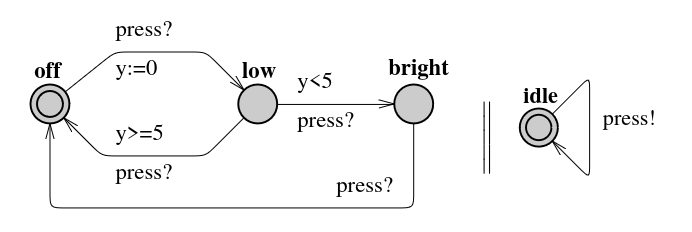
\includegraphics[width=0.8\textwidth]{obrazky-figures/lamp_model.png}
    \caption{Jednoduchý model lampy. Převzato z \cite{uppaal_intro}}
    \label{fig:lamp}
\end{figure}

\subsubsection{Symbolický simulátor a konkrétní simulátor}
\textbf{Symbolický simulátor} je nástroj určený k validaci modelovaného systému. Umožňuje spouštět běhy systému i na začátku návrhu (nebo při modelování) systému, čímž lze objevit chyby ještě před verifikací. Simulátor dále umožňuje vizualizovat běhy systému pomocí tzv. symbolických stop (angl. \textbf{symbolic traces}).

Časový automat se může nacházet v nekonečně mnoho různých stavech, tím pádem může vznikat i nekonečně mnoho konkrétních stop běhu systému. Simulátor není schopen všechny tyto stopy vizualizovat, proto zavádí symbolické stopy. Každý symbolický stav systému v symbolické stopě je sada stavů a jejich následovníků popsaná časovými omezeními. Aktivní lokace a hodnoty diskrétních proměnných jsou stejné pro všechny stavy v symbolickém stavu.

\begin{figure}[H]
    \centering
    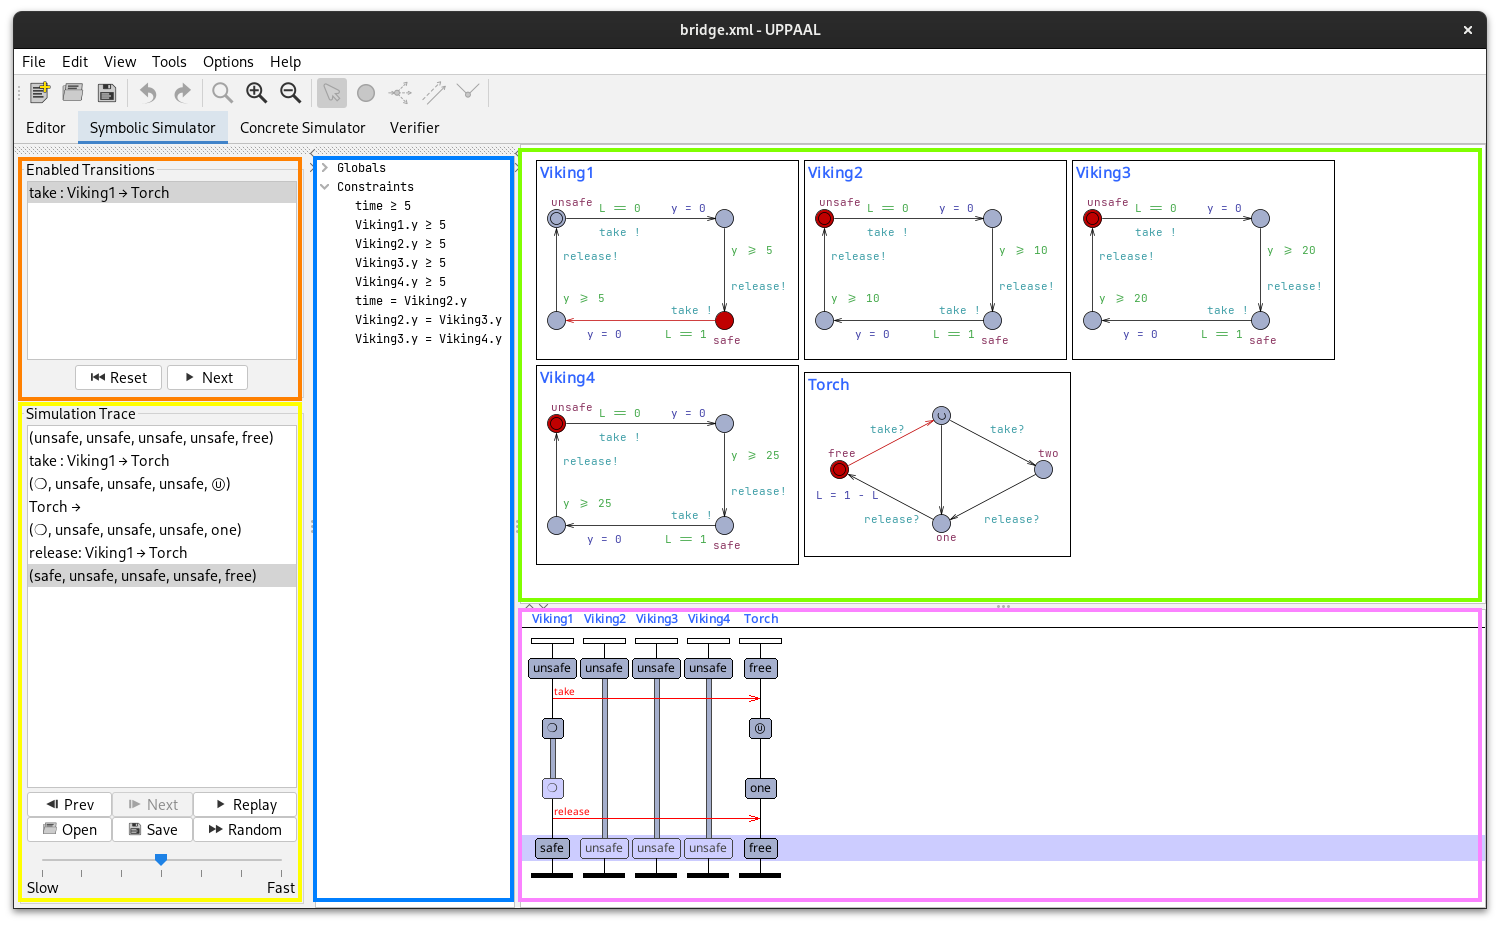
\includegraphics[width=\textwidth]{obrazky-figures/uppaal_symbsim.png}
    \caption{Symbolický simulátor v programu UPPAAL}
    \label{fig:uppaal_symbsim}
\end{figure}

Na obrázku \ref{fig:uppaal_symbsim} jsou barevně rozlišeny jednotlivé součásti simulátoru. Červená část s názvem \textit{Enabled Transitions} slouží ke krokování simulace, uživatel si sám může vybrat, který další přechod se provede. Žlutá část \textit{Simulation Trace} zobrazuje dosavadní vygenerovanou stopu. Dohromady tyto dva elementy slouží k ovládání simulace.

Prostřední modrý panel slouží k zobrazení hodnot globálních a časových proměnných ve stavu systému zvoleném ve výše popsané části \textit{Simulation Trace}. Hodnoty hodin jsou zobrazeny symbolicky jako konjunkce jednotlivých časových omezení (tedy nejsou to přesné hodnoty, ale intervaly, viz např. hodnota \texttt{time $\geq$ 5} na obrázku \ref{fig:uppaal_symbsim}).

V zelené části jsou zobrazeny jednotlivé automaty systému. Jejich aktuální lokace ve vybraném stavu jsou zvýrazněny červenou barvou. V růžové části se nachází tzv. \textit{Message sequence chart}, tedy graf sekvencí zpráv, v rámci něhož lze sledovat komunikaci a synchronizaci jednotlivých automatů systému.

\bigskip

\textbf{Konkrétní simulátor} funguje na podobném principu jako symbolický simulátor, tzn. také slouží k ranné validaci modelů. Odlišuje se tím, že simulace je založena na konkrétních stopách průchodů, takže uživatel může určit, v jaký přesný čas dochází k přechodu do dalšího stavu.

\subsubsection{Verifikátor}
Verifikátor slouží k ověřování bezpečnostních a živostních vlastností (\textit{safety and liveness properties}) systému pomocí procházení symbolického stavového prostoru reprezentovaného omezeními. Dále umožňuje specifikovat a dokumentovat požadavky na systém. Na obrázku \ref{fig:uppaal_verifier} je vidět příklad verifikátoru obsahujícího několik dotazů. Syntaxí a sémantikou dotazů se zabývají podsekce \ref{uppaal_query_lang} a \ref{uppaal_smc_queries}.

\begin{figure}[H]
    \centering
    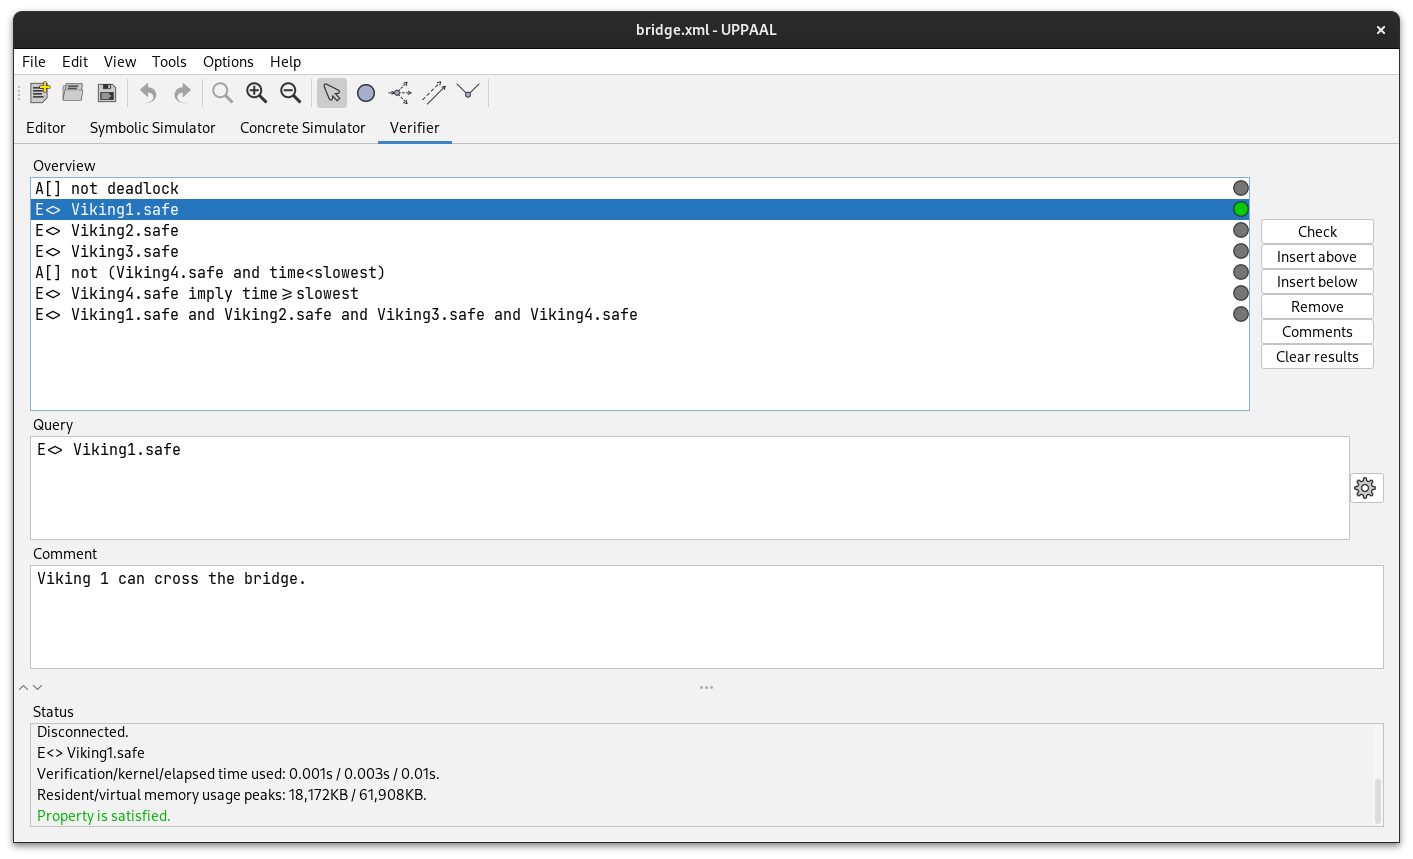
\includegraphics[width=\textwidth]{obrazky-figures/uppaal_verifier.png}
    \caption{Verifikátor programu UPPAAL}
    \label{fig:uppaal_verifier}
\end{figure}

\subsection{Možnosti nastavení parametrů systému}
Tato podsekce se zabývá možnostmi nastavení vstupních parametrů systému, jako jsou různé přístupy k procházení stavového prostoru, stanovení statistických parametrů aj. Je čerpáno z dokumentace UPPAAL \cite{uppaal_doc}.

\subsubsection{Způsob průchodu stavovým prostorem (Search Order)}
K procházení stavového prostoru lze zvolit jeden z následujících přístupů:
\begin{itemize}
    \item průchod do šířky (breadth first search) -- nejefektivnější varianta, pokud je třeba prohledat celý stavový prostor,
    \item průchod do hloubky (depth first search) -- tato varianta je vhodná v případě, že uživatel očekává existenci protipříkladu,
    \item náhodný průchod do hloubky (random depth first search) -- opět vhodné při očekávání existence protipříkladu, nalezená stopa se může kvůli randomizaci při různých bězích lišit.
\end{itemize}

\subsubsection{Redukce stavového prostoru (State Space Reduction)}
Nastavuje, do jaké míry bude program UPPAAL ukládat všechny stavy do paměti. Dochází zde ke hledání kompromisu mezi časovou a paměťovou náročností běhu. Možnosti jsou následující:
\begin{itemize}
    \item Žádná (None) -- ukládá všechny stavy do paměti,
    \item Konzervativní (Conservative) -- neukládá tzv. zavázané stavy (\textit{commited states}),
    \item Agresivní (Aggresive) -- neukládá více než jeden stav za cyklus.
\end{itemize}

\subsubsection{Reprezentace stavového prostoru (State Space Representation)}
Určuje, jakým způsobem má být stavový prostor reprezentován. U některých aproximativních reprezentací může docházet k tomu, že výsledek dotazu je \uv{možná} splněn, tedy že program UPPAAL nedokáže jednoznačně určit výsledek. Možnosti reprezentace jsou následující:
\begin{itemize}
    \item Rozdílové matice (Difference Bound Matrices, DBM) -- rychlé, u modelů s mnoha časovými proměnnými spotřebují velké množství paměti,
    \item Kompaktní datová struktura (Compact Data Structure) -- kompaktnější (menší spotřeba paměti) a pomalejší než DBM,
    \item Nedostatečná aproximace (Under Approximation) -- využívá hashovací tabulky, míra aproximace lze nastavit určením velikosti dané tabulky (možnost \textit{Hash Table Size} v nastavení),
    \item Nadměrná aproximace (Over Approximation) -- využívá komplexní obaly k aproximaci zón, nemá žádný efekt u modelů bez časových proměnných.
\end{itemize}

\subsubsection{Statistické parametry}
\begin{itemize}
    \item \textbf{Dolní pravděpodobnostní odchylka} (Lower probabilistic deviation) ($-\delta$) -- používána při testování hypotéz pro určení spodní hranice indiferenční oblasti od zadané pravděpodobnosti.
    \item \textbf{Horní pravděpodobnostní odchylka} (Upper probabilistic deviation) ($+\delta$) -- používána při testování hypotéz pro určení horní hranice indiferenční oblasti od zadané pravděpodobnosti.
    \item \textbf{Pravděpodobnost falešně pozitivních výsledků} (Probability of false positives) ($\alpha$) -- používána při testování hypotéz a odhadu pravděpodobnosti k určení míry statistické významnosti. Jedná se o pravděpodobnost tzv. chyby typu I (\textit{Type I error}), což je chybné zamítnutí nulové hypotézy.
    \item \textbf{Pravděpodobnost falešně negativních výsledků} (Probability of false negatives) ($\beta$) -- používána při testování hypotéz k určení míry statistické významnosti. Jedná se o pravděpodobnost tzv. chyby typu II (\textit{Type II Error}), tedy chybné potvrzení nulové hypotézy.
    \item \textbf{Neurčitost pravděpodobnosti} (Probability uncertainty) ($\varepsilon$) -- používána při odhadu pravděpodobnosti k omezení velikosti konfidenčního intervalu ve tvaru $p \pm \varepsilon$.
    \item \textbf{Dolní a horní hranice poměru} (Ratio lower bound a Ratio upper bound) ($u_0$, $u_1$) -- používány při porovnávání dvou pravděpodobností.
    \item Nastavení šířky a počtu sloupců v histogramech.
\end{itemize}

\subsection{Dotazovací jazyk} \label{uppaal_query_lang}
Tato podsekce čerpá z článků \cite{uppaal_intro} a \cite{uppaal_smc}. Hlavním úkolem nástroje na ověřování modelů je verifikace modelu s ohledem na určité požadavky. Takové požadavky musejí být vyjádřeny v nějakém formálně definovaném a strojově čitelném jazyce. Existuje několik logik, které toto splňují, UPPAAL používá zjednodušenou verzi logiky TCTL (\textit{Timed Computation Tree Logic}). Dotazovací jazyk se tedy, podobně jako v TCTL, skládá ze stavových formulí (\textbf{state formulae}) a běhových formulí (\textbf{path formulae}). Stavové formule popisují jednotlivé stavy systému, běhové formule kvantifikují přes jednotlivé běhy nebo stopy systému.

Příklady běhových formulí lze pozorovat na obrázku \ref{fig:uppaal_path_form}. Stavy, které splňují danou stavovou formuli $\varphi$, jsou vybarveny žlutě. Hrany, které jsou procházeny při vyhodnocování, jsou ztučněny. Významy jednotlivých běhových formulí jsou vysvětleny níže ve zbytku podsekce.

\begin{figure}[H]
    \centering
    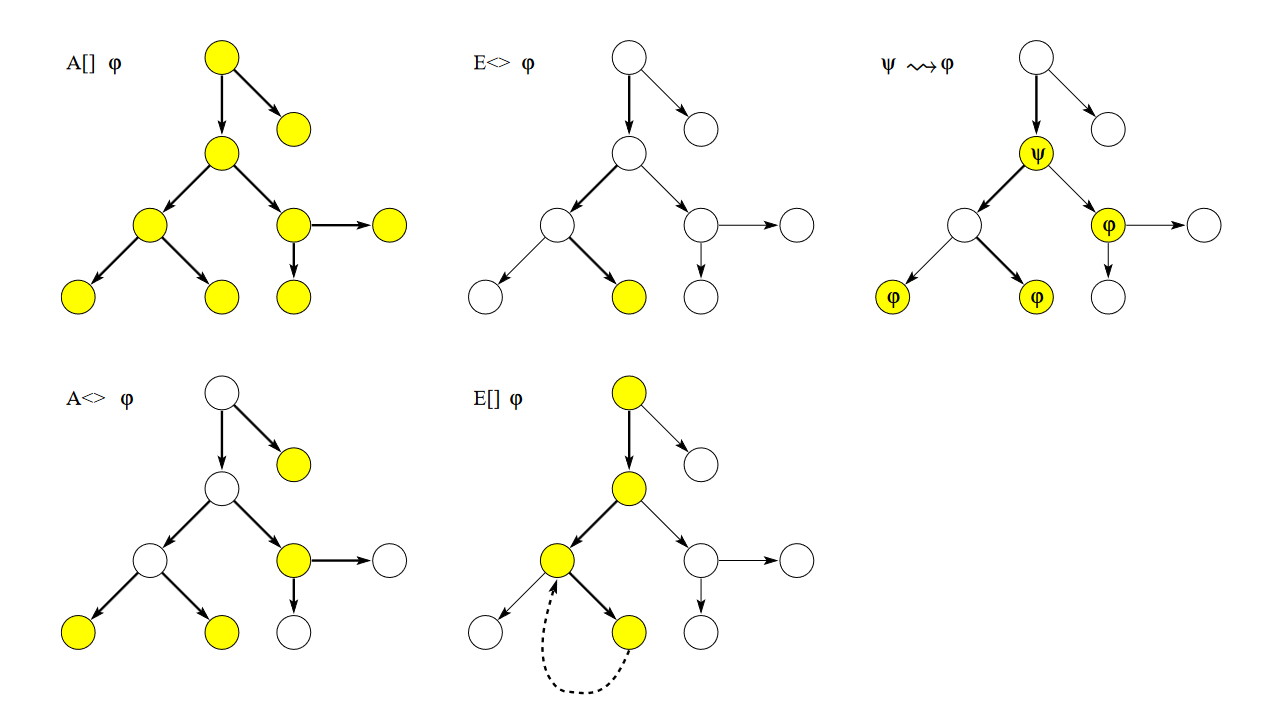
\includegraphics[width=\textwidth]{obrazky-figures/uppaal_path_form.png}
    \caption{Běhové formule v nástroji UPPAAL. Převzato z \cite{uppaal_intro}}
    \label{fig:uppaal_path_form}
\end{figure}

\subsubsection{Stavové formule}
Stavová formule je výraz, který může být vyhodnocen pro nějaký stav modelu bez ohledu na jeho chování. Příkladem může být jednoduchý výraz \texttt{i == 7}, který bude platit tehdy, pokud se v daném stavu $i$ rovná 7. Syntax stavových formulí je nadmnožinou syntaxe časových omezení, u stavových formulí je navíc možné použití disjunkce. Dále je možno otestovat, zda se proces nachází v určité lokaci pomocí výrazu \texttt{P.1}, kde \texttt{P} je proces a \texttt{1} je lokace.

\subsubsection{Dosažitelnost}
Dotazy na dosažitelnost se snaží zjistit, zda je daná stavová formule $\varphi$ splnitelná nějakým dosažitelným stavem. Jinými slovy zda existuje cesta z počátečního stavu taková, že je během ní $\varphi$ eventuelně splněno. Například při návrhu modelu nějakého komunikačního protokolu, v němž figurují odesílatel a příjemce, lze dotaz na dosažitelnost využít k ověření, že odesílatel může vůbec někdy poslat zprávu, nebo že ji příjemce eventuelně může přijmout.

K vyjádření, že by nějaký stav $\varphi$ měl být eventuelně dosažitelný, lze použít běhovou formuli $E \diamond \varphi$. V syntaxi programu UPPAAL je to \texttt{E<> $\varphi$}.

\subsubsection{Bezpečnost}
Dotazy na bezpečnost zajišťují, že nikdy nenastane \uv{něco špatného}. Příkladem může být sledování teploty v nějakém modelu elektrárny a nastavení hodnoty, přes kterou by se teplota nikdy neměla dostat. Jinou variantou tohoto dotazu je dotaz \uv{Něco se možná nikdy nestane.} Například při hraní hry je stav bezpečný, pokud v něm stále má hráč šanci vyhrát, tedy možná neprohraje.

V nástroji UPPAAL jsou tyto dotazy formulovány kladně, tedy \uv{Něco správného vždy platí.} Pro stavovou formuli $\varphi$ lze dosažitelnost ve všech stavech vyjádřit běhovou formulí $A \square \varphi$ (v syntaxi UPPAAL je to \texttt{A[] $\varphi$}). Pomocí běhové formule $E \square \varphi$ (v syntaxi UPPAAL \texttt{E[] $\varphi$}) lze vyjádřit, že by měla existovat maximální cesta taková, že $\varphi$ vždy platí. Maximální cesta je taková cesta, která je buď nekonečná, nebo končí ve stavu, z něhož nevedou žádné další přechody.

\subsubsection{Živost}
Dotazy na živost (angl. \textit{liveness}) ověřují, že se něco eventuelně stane. Například pokud došlo ke stisknutí tlačítka pro spuštění televize, že se televize eventuelně spustí, nebo že zpráva, která byla odeslána v rámci nějakého komunikačního protokolu, bude eventuelně doručena.

V nejjednodušší formě lze tyto dotazy zapisovat jako $A \diamond \varphi$, tedy že stavová formule $\varphi$ je eventuelně splněna. Složitější a užitečnější je forma dotazu $\varphi \rightsquigarrow \psi$ vyjadřující situaci \uv{Vždy, když je splněno $\varphi$, bude eventuelně později splněno i $\psi$}. V programu UPPAAL tyto dotazy zapisujeme jako \texttt{A<> $\varphi$}, respektive \texttt{$\varphi$ ----> $\psi$}.

\subsection{Rozšíření dotazovacího jazyka v rámci UPPAAL SMC} \label{uppaal_smc_queries}
Zdrojem této podsekce je článek \cite{uppaal_smc}. UPPAAL SMC rozšiřuje dotazovací jazyk o nové dotazy zaměřené na stochastickou interpretaci časových automatů. Také umožňuje uživatelům vizualizovat hodnoty výrazů a proměnných přímo v průběhu simulačních běhů. Syntax takových dotazů je následující:
\begin{equation*}
    \texttt{simulate [<=bound;N] \{ E1,...,Ek \}},
\end{equation*}
kde \texttt{N} je přirozené číslo určující počet simulací, které se mají provést, \texttt{bound} je časová hranice jednotlivých simulací a \texttt{E1,...,Ek} jsou jednotlivé výrazy, které mají být monitorovány a vizualizovány. Příkladem může být dotaz používaný v praktické části práce k vizualizaci výsledků výpočtů přesné násobičky (proměnná \texttt{res\_acc}) a zkoumané přibližné násobičky (proměnná \texttt{res\_approx}):

\begin{equation*}
    \texttt{simulate [<=20000;1] \{ res\_acc, res\_approx \}}
\end{equation*}

Výslednou vizualizaci je možno vidět na obrázku \ref{fig:simulate_example}. Nástroj UPPAAL také umožňuje export dat ve formátu csv, čehož lze využít při další podrobnější analýze.

\begin{figure}[H]
    \centering
    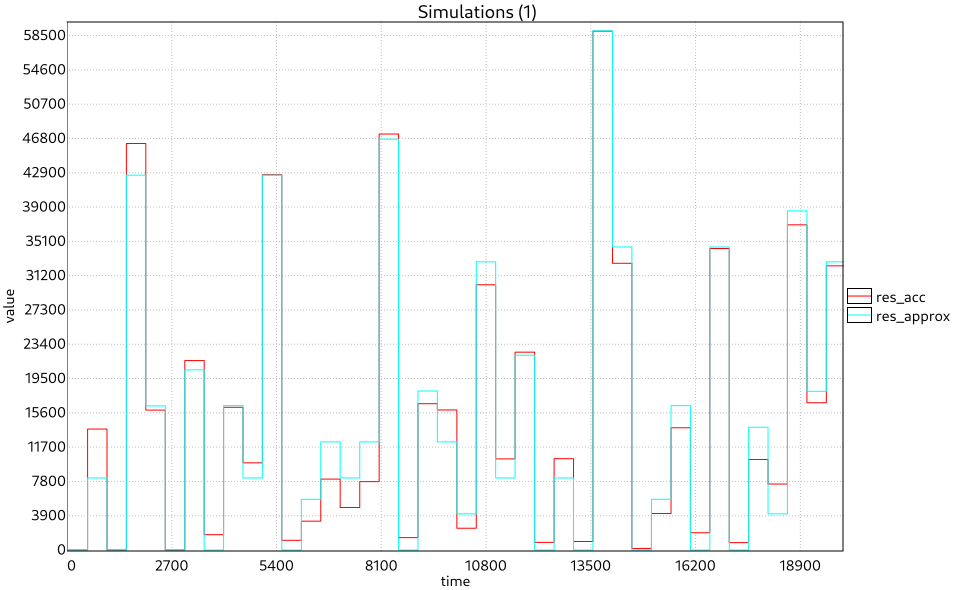
\includegraphics[width=\textwidth]{obrazky-figures/simulate_example.png}
    \caption{Vizualizace hodnot při simulaci, nástroj UPPAAL}
    \label{fig:simulate_example}
\end{figure}

\subsubsection{Odhad pravděpodobnosti}
Dotazy kvantitativního ověřování modelů mají následující syntax:

\begin{equation*}
    \texttt{Pr[<=bound;N](<>|[] expression)}
\end{equation*}

Výsledkem takového dotazu je interval spolehlivosti odhadu pravděpodobnosti, s jakou bude běhová formule \texttt{<>|[] expression} platná za předpokladu, že platí výraz \texttt{bound}. Jako hranice \texttt{bound} lze typicky zvolit nějaké časové omezení, ať už omezení globálního času, konkrétních hodin nebo třeba počet kroků (diskrétních přechodů). Konfidenční hladinu intervalu spolehlivosti lze modifikovat parametry $\alpha$ a $\epsilon$ v nastavení nástroje UPPAAL.

\subsubsection{Testování hypotéz}
Testování hypotéz, neboli kvalitativní ověřování modelů, zjišťuje, zda je pravděpodobnost platnosti nějakého výrazu vyšší nebo nižší než nějaká daná hodnota (\texttt{prob\_number}). Je efektivnější než dotaz na odhad pravděpodobnosti, protože je jednostranné, tudíž je potřeba méně simulací k dosažení stejně významného výsledku. Syntax je následující:

\begin{equation*}
    \texttt{Pr[<=bound;N] (<>|[] expression) <=|>= prob\_number}
\end{equation*}

\subsubsection{Porovnání pravděpodobností}
Tento dotaz nepřímo porovnává dvě pravděpodobnosti, aniž by je odhadoval. Syntax je následující:

\begin{equation*}
    \texttt{Pr[<=bound1;N1] (<>|[] expression1) >= Pr[<=bound2;N2] (<>|[] expression2)}
\end{equation*}

\subsubsection{Odhad hodnoty}
Umožňuje odhadnout maximální nebo minimální hodnotu určité proměnné (pouze integer nebo hodiny) v rámci časového omezení \texttt{bound}. Syntax je následující:

\begin{equation*}
    \texttt{E[<=bound;N] (min|max: expression)}
\end{equation*}

Příklad využití z praktické části práce odhaduje maximální zpoždění vzniklé při výpočtu jednoho výsledku přibližné násobičky. Časové omezení je stanoveno na 20000 jednotek, také je v dotazu explicitně stanoveno 5 simulačních běhů:

\begin{equation*}
    \texttt{E[<=20000;5] (max: current\_delay)}
\end{equation*}

Výsledkem dotazu je konfidenční interval s předem danou hladinou spolehlivosti. Výsledkem tohoto konkrétního dotazu při simulaci jedné konkrétní náhodně vybrané přibližné násobičky byla hodnota \texttt{1138 +- 18.4169 (95\% CI)}. 

Jak lze vidět na obrázku \ref{fig:prob_plots}, nástroj UPPAAL dále umožňuje některé detailnější pohledy na odhad dané hodnoty. Konkrétně se jedná o grafy rozdělení hustoty pravděpodobnosti (\textit{Probability Density Distribution}), rozdělení pravděpodobnosti (\textit{Probability Distribution}), rozdělení distribuční funkce pravděpodobnosti (\textit{Cumulative Probability Distribution}), zobrazení konfidenčních intervalů distribuční funkce (\textit{Cumulative Probability Confidence Intervals}) a také histogram frekvencí výskytu jednotlivých hodnot při simulačních bězích (\textit{Frequency Histogram}).

\begin{figure}[H]
    \centering
    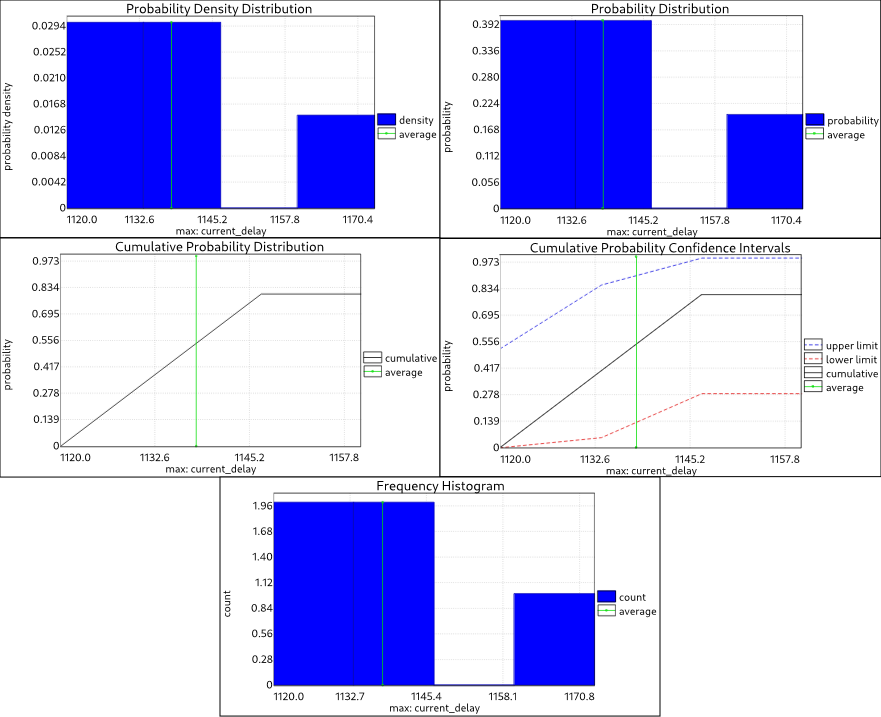
\includegraphics[width=0.9\textwidth]{obrazky-figures/prob_plots.png}
    \caption{Grafy pravděpodobnostního rozdělení při odhadu maximální hodnoty proměnné v nástroji UPPAAL}
    \label{fig:prob_plots}
\end{figure}

\chapter{Návrh a implementace řešení}
\label{rozbor}
Hlavním cílem praktické části bakalářské práce bylo vytvoření modelů zástupců zvolené třídy přibližných výpočetních systémů (angl. \textit{Approximate Computing}, zkratka AC), ověření jejich vlastností pomocí prostředků SMC a porovnání těchto vlastností s vlastnostmi přesných variant daných výpočetních systémů.

Jako třída zkoumaných AC systémů byly zvoleny násobičky. Práce navazuje zejména na článek \cite{smc_axc}, tedy na práci vedoucího této bakalářské práce dr. Strnadela. Konkrétně přebírá systém modelů sloužící k simulaci násobení přesné a přibližné násobičky 2x2 bity a rozšiřuje jej o následující prvky:
\begin{itemize}
    \item rozšíření systému pro větší násobičky (až 11x11 bitů),
    \item výpočet chybových metrik popsaných v části \ref{error_metrics},
    \item sledování počtu překlopení bitů (\textit{bit flips}) při jednotlivých výpočtech,
    \item sledování zpoždění při jednotlivých výpočtech,
    \item generování vstupů s různým pravděpodobnostním rozdělením.
\end{itemize}

Jako zdroj modelů přibližných násobiček byla zvolena knihovna EvoApproxLib \cite{circuit_library}. Tato knihovna poskytuje dohromady několik stovek modelů přibližných násobiček a sčítaček jak v bezznaménkové, tak znaménkové variantě. Tato práce se zaměřuje na bezznaménkové násobičky, zejména na variantu 8x8 bitů, ale implementovaný překladač (viz sekce \ref{parser}) lze použít i pro násobičky 7x7 a 11x11 bitů.

\bigskip

Předmětem zkoumání bylo porovnávání vlastností přibližných násobiček při generování vstupních hodnot podle různých pravděpodobnostních rozdělení. Základní osnova postupu řešení vypadala následovně:

\begin{itemize}
    \item nasbírání dat (násobených dvojic čísel) z vybraných algoritmů a vizualizace dat,
    \item tvorba pravděpodobnostních rozdělení pro generování náhodných čísel podle reálných rozdělení násobených čísel v implementacích algoritmů,
    \item implementace \uv{překladače}, který převádí modely přibližných násobiček z knihovny EvoApproxLib \cite{circuit_library} napsaných v jazyce Verilog do modelů v nástroji UPPAAL,
    \item vytvoření simulačních dotazů ve verifikátoru nástroje UPPAAL,
    \item simulace různých kombinací násobiček a náhodných rozdělení, 
    \item zpracování a vizualizace výsledků.
\end{itemize}

\begin{figure}[H]
    \centering
    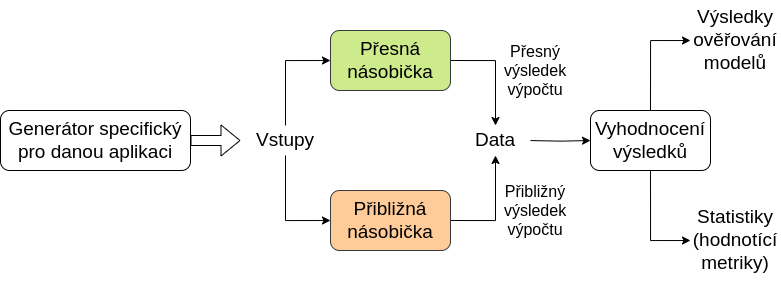
\includegraphics[width=0.8\textwidth]{obrazky-figures/acc_approx_diagram.png}
    \caption{Schéma systému porovnávání výstupů přesné a přibližné násobičky}
    \label{fig:acc_approx_diagram}
\end{figure}

Tato kapitola se zabývá podrobnějším popisem návrhu a řešení výše zmíněných bodů.

\section{Popis systému v nástroji UPPAAL}
Tato sekce se věnuje popisu systému modelů v nástroji UPPAAL. Zaměřuje se především na popis jednotlivých modelů -- časových automatů, dále jsou zmíněny některé důležité proměnné a funkce a také je nastíněna celková synchronizace systému.

\subsection{Globální deklarace}
V rámci globálních deklarací dochází k vytvoření základního rozhraní systému. Nejdůležitější součásti jsou zobrazeny ve výpise \ref{lst:interface}. 

Jedná se o definici počtu vstupních a výstupních bitů systému (tedy kolik bitů mají 2 vstupní hodnoty a kolik bitů má 1 výstupní hodnota) v proměnných \texttt{NPI}, resp. \texttt{NPO}. Dále je deklarováno pole pravdivostních hodnot \texttt{bits}, které slouží jak k uložení bitů vstupních a výstupních hodnot, tak také k uložení dílčích výstupů jednotlivých logických hradel. Každé hradlo má svoje unikátní ID, které slouží jako index do pole \texttt{bits}, kam ukládá výsledek svojí operace, a odkud jej poté mohou další hradla načíst.

Indexy bitů vstupních a výstupních hodnot jsou definovány v polích \texttt{PIxy}, respektive \texttt{POx} (výstup přesné násobičky) a \texttt{POy} (výstup přibližné násobičky).

\begin{lstlisting}[language={C}, caption={Základní rozhraní systému}, label={lst:interface}]
const NPI = 16; //number of input bits
const NPO = 16; //number of output bits

const int MAX_BITS = 1024;
bool bits[MAX_BITS];

//indexes of input bits for both input numbers
const int PIxy[NPI] = {0, 1, 2, 3, 4, 5, 6, 7, 8,
    9, 10, 11, 12, 13, 14, 15};

//indexes of bits of accurate mult. output
const int POx[NPO] = {16, 17, 18, 19, 20, 21, 22,
    23, 24, 25, 26, 27, 28, 29, 30, 31};

//indexes of bits of approx. mult. output
const int POy[NPO] = {32, 33, 34, 35, 36, 37, 38,
    39, 40, 41, 42, 43, 44, 45, 46, 47};
\end{lstlisting}

Dále zde dochází k deklaracím a definicím řady pomocných proměnných a funkcí, zejména všech proměnných obsahujících výsledky výpočtů sledovaných chybových metrik, dále také funkce porovnávající výsledky výpočtů přesné a přibližné násobičky aj.

\subsection{Modely}
V této podsekci jsou zobrazeny a popsány jednotlivé používané modely.

\subsubsection{Model přesné násobičky}
Modeluje kombinační obvod přesné násobičky definovaný pomocí pravdivostní tabulky. Po inicializaci model čeká na signál kanálu \texttt{update}, který značí vygenerování nových vstupních hodnot. Poté v rámci funkce \texttt{f()} vygeneruje výsledek výpočtu pro kombinaci vstupů a pravdivostní tabulky a uloží jej do globální proměnné \texttt{bits}. Po uběhnutí \texttt{dly} časových jednotek se vrací do stavu čekání na další vstupní hodnoty.

\begin{figure}[H]
    \centering
    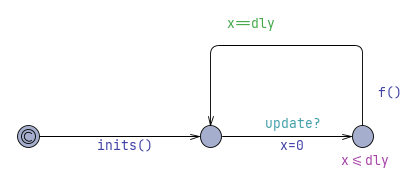
\includegraphics[width=0.6\textwidth]{obrazky-figures/model_tmul2any.png}
    \caption{Časový automat reprezentující model přesné násobičky}
    \label{fig:model_tmul2any}
\end{figure}

\subsubsection{Model generátoru vstupů}
Model generátoru pseudonáhodných čísel -- dvou vstupních hodnot pro přesnou i přibližnou násobičku. Po inicializaci model pomocí funkce \texttt{f(idx)} vygeneruje nové hodnoty a rozešle synchronizační signál v kanále \texttt{update}. Pomocí funkce \texttt{inCovered} sleduje, zda byly vygenerovány všechny možné vstupní kombinace. Pokud ano, ukončuje generování a přechází do lokace \texttt{done}. Jinak čeká na signál z kanálu \texttt{cmpDone} a poté generuje další dvojici hodnot.

\begin{figure}[H]
    \centering
    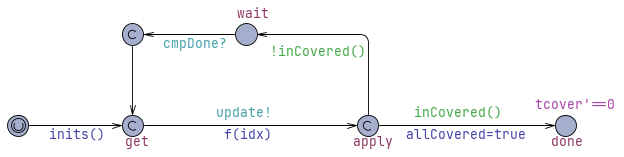
\includegraphics[width=0.9\textwidth]{obrazky-figures/model_tmul2_tb_random.png}
    \caption{Časový automat reprezentující model generátoru pseudonáhodných veličin}
    \label{fig:model_tmul2_tb_random}
\end{figure}

\subsubsection{Model kontroly rovnosti}
Tento model provádí kontrolu rovnosti výsledků přibližné a přesné násobičky. Model čeká ve své počáteční lokaci, dokud nejsou připraveny výsledky jak přesného, tak přibližného výpočtu (\texttt{diffctrl==2}). Poté v rámci volání funkce \texttt{diff()} provede porovnání výsledků a také průběžné výpočty všech sledovaných metrik. Po dokončení všech výpočtů odesílá signál v kanále \texttt{cmpDone} značící, že porovnávání bylo dokončeno, a vrací se do počáteční lokace.

\begin{figure}[H]
    \centering
    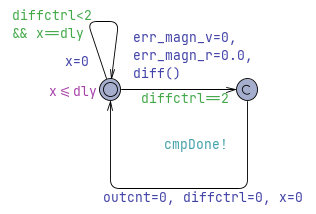
\includegraphics[width=0.45\textwidth]{obrazky-figures/model_eval_diff.png}
    \caption{Časový automat reprezentující model kontroloru rovnosti výsledků}
    \label{fig:model_eval_diff}
\end{figure}

\subsubsection{Model synchronizace vstupních hodnot}
Model čeká na vygenerování nových vstupních hodnot (tedy na signál \texttt{update?}). Poté pomocí kanálu \texttt{change[idx]} postupně dává signál jednotlivým logickým členům, že byl jejich vstupní bit aktualizován. Proměnná \texttt{idx} představuje pozici jednotlivých bitů. Model iteruje mezi dvěma zavázanými lokacemi tak dlouho, dokud se neprojde přes všechny vstupní bity (konstantní proměnná \texttt{NPI} značí počet vstupních bitů násobičky). Po aktualizování všech bitů se model vrací do počáteční lokace.

\begin{figure}[H]
    \centering
    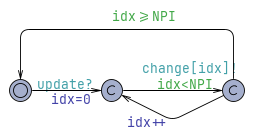
\includegraphics[width=0.4\textwidth]{obrazky-figures/model_syncPrimary.png}
    \caption{Časový automat reprezentující model zajišťující synchronizaci vstupních hodnot}
    \label{fig:model_syncPrimary}
\end{figure}

\subsubsection{Model logického hradla}
Modeluje logický člen se dvěma vstupy a jedním výstupem. Model při inicializaci přijímá následující vstupní parametry:
\begin{equation*}
    \begin{array}{l}
       \texttt{const int id, const int a0, const int a1, const int y0,} \\
       \texttt{broadcast chan \&cin0, broadcast chan \&cin1, broadcast chan \&cout0,}
    \end{array}
\end{equation*}
kde konstanta \texttt{id} je jedinečný identifikátor daného hradla. Konstatní proměnné \texttt{a0} a \texttt{a1} značí pozice vstupních bitů v globálním poli \texttt{bits}, konstanta \texttt{y0} je pozice výstupního bitu ve stejném poli. Broadcastové synchronizační kanály \texttt{cin1} a \texttt{cin2} slouží k přijetí signálu o tom, že byl jeden ze vstupních bitů aktualizován (jedná se tedy o kanál \texttt{change} zmíněný výše u modelu synchronizace). Přes synchronizační kanál \texttt{cout0} rozesílá hradlo signál o aktualizaci svého výstupního bitu. Tento signál poté přijímají všechna další hradla, která používají jeho výstupní bit jako svůj vstupní bit.

Po inicializaci model čeká na aktualizace jednoho ze vstupních bitů (kanály \texttt{cin0} a \texttt{cin1}). Poté dochází k vygenerování výstupu (\texttt{outGen(tbl\_op[id])}) a po uběhnutí zpoždění signálu (\texttt{x == duration(tbl\_op[id])}) se model vrací zpět do lokace čekání na nové vstupy.

Hradla mohou vykonávat následující logické operace: AND, NAND, OR, NOR, XOR a XNOR. Každé hradlo má svoji operaci uloženou v poli \texttt{tbl\_op} na pozici \texttt{id}. Zpoždění jednotlivých operací se liší, pro každou z nich je definováno v rámci globální funkce \texttt{duration}.

\begin{figure}[H]
    \centering
    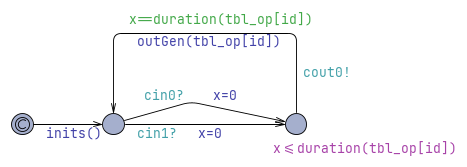
\includegraphics[width=0.6\textwidth]{obrazky-figures/model_gate2.png}
    \caption{Časový automat reprezentující model logického hradla}
    \label{fig:model_gate2}
\end{figure}

\subsection{Inicializace systému}
V závěru dochází k inicializace a propojení celého systému. Ve výpise \ref{lst:init} je vidět inicializace jednotlivých součástí. \texttt{synPri} představuje model synchronizace, \texttt{ediff} zase model kontroly rovnosti. \texttt{mul2A} je model přesné násobičky, \texttt{mul2Atb} představuje generátor náhodných vstupních hodnot. Na konci lze pozorovat inicializaci jednotlivých logických hradel \texttt{gate2}.

\begin{lstlisting}[language={C}, caption={Inicializace systému}, label={lst:init}]
synPri = syncPrimary();

mul2A = tmul2any(PIxy, POx, tbl_acc_any, DLY_MUL2);
mul2Atb = tmul2_tb_random(DLY_MUL2, COVERAGE_RATIO);

ediff = eval_diff(5);

//gates
g122=gate2(0, PIxy[14], PIxy[0], 122, change[14], change[0], change[122]);
g123=gate2(1, PIxy[15], PIxy[0], 123, change[15], change[0], change[123]);
g127=gate2(2, PIxy[10], PIxy[4], 127, change[10], change[4], change[127]);
g129=gate2(3, PIxy[13], PIxy[1], 129, change[13], change[1], change[129]);
g130=gate2(4, PIxy[14], PIxy[1], 130, change[14], change[1], change[130]);
g133=gate2(5, PIxy[15], PIxy[1], 133, change[15], change[1], change[133]);
g142=gate2(6, 122, 129, 142, change[122], change[129], change[142]);
//...
//...
//...
g433=gate2(214, 431, 430, 433, change[431], change[430], change[433]);
g434=gate2(215, 431, 430, POy[14], change[431], change[430], change[434]);
g435=gate2(216, 432, 433, POy[15], change[432], change[433], change[435]);
g436=gate2(217, 318, 210, POy[3], change[318], change[210], change[436]);
\end{lstlisting}

\section{Převod modelů z jazyka Verilog do modelů v nástroji UPPAAL} \label{parser}
Jak již bylo zmíněno, zdrojem modelů přibližných bezznaménkových násobiček je knihovna EvoApproxLib \cite{circuit_library}. K překladu těchto modelů do modelů v prostředí UPPAAL byl implementován skript v jazyce Python nazvaný \texttt{parse.py}.

Skript je schopen přeložit modely z jazyka Verilog ve formátu zobrazeném ve výpise \ref{lst:verilog}. Zvládne tedy přeložit všechny modely násobiček 7x7, 8x8 (kromě násobičky \texttt{mul8u\_1JJQ}) a 11x11 bitů. Modely násobiček 12x12 a 16x16 bitů mají odlišnou (složitější) strukturu. Jsou modelovány pomocí skládání menších přibližných násobiček do sebe a skript \texttt{parse.py} toto neimplementuje.

\begin{figure}[H]
    \centering
    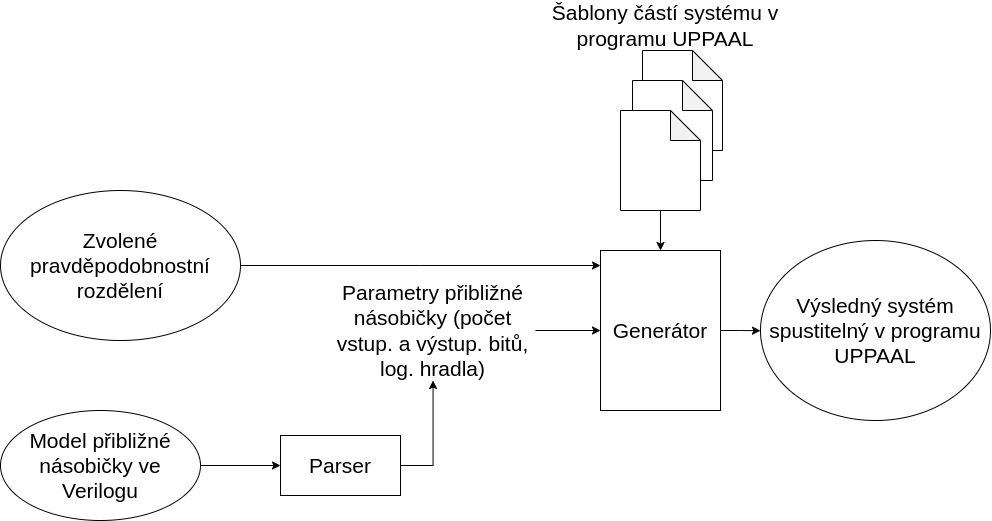
\includegraphics[width=0.9\textwidth]{obrazky-figures/parser_diagram.png}
    \caption{Schéma fungování skriptu \texttt{parse.py}}
    \label{fig:parser_diagram}
\end{figure}

\begin{lstlisting}[language={Verilog}, caption={Příklad platného formátu modelu násobičky v jazyce Verilog}, label={lst:verilog}]
module mult_name (
    A,
    B,
    O
);

input [n:0] A;
input [n:0] B;
output [m:0] O;

wire sig_10,sig_11, ...;

assign sig_10 = A[0] & B[1];
...
assign sig_30 = sig_15 & sig_20;
...

assign O[15] = sig[30];
...
assign O[0] = 1'b0;
\end{lstlisting}

\subsubsection{Základní princip fungování skriptu}
Pseudokód struktury funkce \texttt{main} skriptu \texttt{parse.py} je k vidění ve výpise \ref{lst:main}.
\begin{lstlisting}[language={Python}, caption={Pseudokód hlavní části skriptu parse.py}, label={lst:main}]
read(input_file)

for line in input_file:
    parse_input_output(line)

create_PIxy_mapping()
create_POy_mapping()

for line in input_file:
    parse_gates(line)

generate_parts()
output_file = join_parts()

write(output_file)
\end{lstlisting}

Prvním krokem je otevření a načtení vstupního souboru napsaného ve Verilogu. Při první iteraci přes jednotlivé řádky souboru je získána informace o počtu vstupních a výstupních bitů násobičky. Ta je využita k nastavení některých vnitřních parametrů skriptu a také k pozdějšímu vygenerování globálních proměnných \texttt{NPI}, \texttt{NPO} a polí \texttt{PIxy}, \texttt{POx} a \texttt{POy}.

Při druhé iteraci přes jednotlivé řádky vstupního souboru dochází k vytváření instancí logických hradel. Na obrázku \ref{fig:sig_to_gate} je vidět princip převodu logické operace dvou signálů ze vstupního souboru na instanci hradla \texttt{gate2} v prostředí UPPAAL. Části, které se na sebe vzájemně mapují, jsou odlišeny barevně. Také je vidět uložení typu logické operace do tabulky \texttt{tbl\_op}. ID hradla, které se používá jako index do tabulky (v tomto příkladě hodnota 0), je s každým hradlem postupně inkrementováno a začíná vždy od 0 bez ohledu na další hodnoty.

Na obrázku \ref{fig:sig_to_gate} lze pozorovat dvě varianty parametrů. V části (a) se jedná o logické hradlo, které přebírá výsledky operací z předchozích hradel. Hradlo v části (b) má na vstupu přímo vstupní bity násobičky \texttt{B[0]} a \texttt{A[0]}. Dále se v modelech vyskytují různé kombinace těchto a dalších variant, princip jejich překladu ovšem zůstává stejný.

\begin{figure}[H]
    \centering
    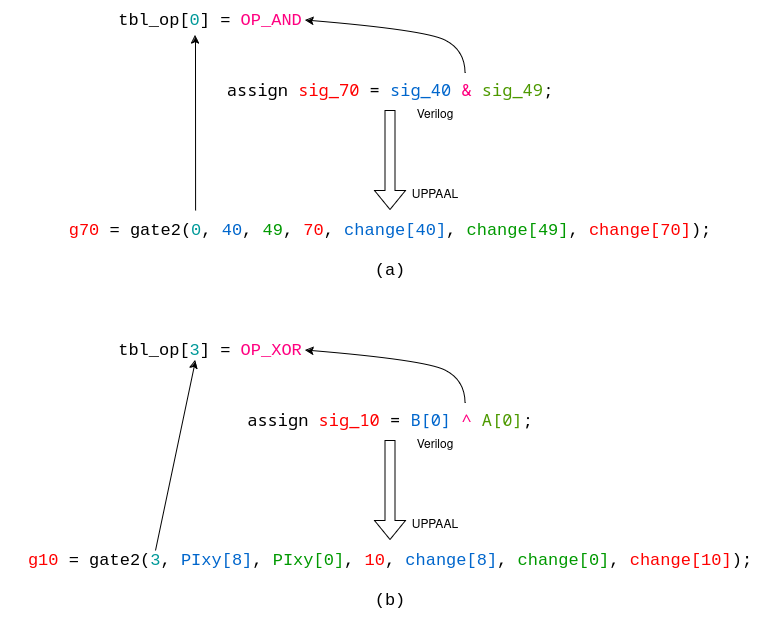
\includegraphics[width=0.9\textwidth]{obrazky-figures/sig_to_gate.png}
    \caption{Vytvoření instance logického hradla v nástroji UPPAAL z předlohy ve Verilogu}
    \label{fig:sig_to_gate}
\end{figure}

Na konci vstupního souboru dochází k přiřazování jednotlivých signálů k výstupním bitům. To je ve skriptu řešeno tak, že se podle čísla v názvu signálu vyhledá hradlo se stejným číslem v názvu a v jeho parametrech se aktualizuje index výstupního bitu na index \texttt{POy[n]} značící index výstupního bitu celé přibližné násobičky (viz obrázek \ref{fig:gate_output}).

\begin{figure}[H]
    \centering
    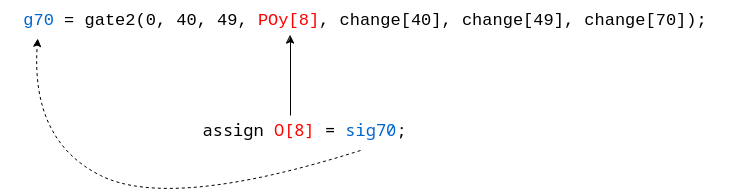
\includegraphics[width=0.9\textwidth]{obrazky-figures/gate_output.png}
    \caption{Aktualizace výstupního bitu logického hradla}
    \label{fig:gate_output}
\end{figure}

V závěru skriptu poté dochází k vygenerování jednotlivých částí výstupního souboru. Soubory systémů v programu UPPAAL jsou napsány v jazyce XML, neboť jejich součástí jsou i grafické objekty (modely časových automatů) definované pomocí uzlů XML. Vygenerované části jsou nakonec spojeny a uloženy do výstupního souboru, s nímž je poté možné pracovat v programu UPPAAL.

Skript lze spouštět s přepínačem \texttt{----distribution [DISTRIBUTION]}, který nastavuje vybrané pravděpodobnostní rozdělení pro generování náhodných vstupů. Při vytváření modelu generátoru náhodných vstupů je poté vybrané rozdělení zohledněno. Rozdělení jsou ve skriptu připravena pro násobičky 8x8 bitů (tedy generují čísla 0 až 255). Pro jiné typy násobiček by bylo třeba tyto hodnoty změnit, případně je lze změnit po vygenerování ve finálním souboru v lokálních deklaracích modelu \texttt{tmul2\_tb\_random}.

\section{Zvolená pravděpodobnostní rozdělení při generování náhodných vstupů} \label{rozdeleni_pst}
Klíčovou myšlenkou práce bylo ověření vlastností přibližných násobiček v závislosti na různých pravděpodobnostních rozděleních jejich vstupů. V rámci této práce bylo zvoleno několik algoritmů, u nichž dochází k násobení celých kladných čísel. Každý algoritmus byl s vhodnými vstupy simulován s tím, že se postupně sbírala data o dvojicích násobených čísel. Tato data byla poté vizualizována a následně byl proveden odhad pravděpodobnostního rozdělení (nebo kombinace více rozdělení), které by přibližně odpovídalo danému naměřenému rozdělení.

Výchozím a referenčním rozdělením bylo zvoleno rozdělení nazvané \textbf{uni\_uni}. Oba vstupy jsou v tomto případě generovány s rovnoměrným rozdělením v intervalu 0 až 255 (minimální a maximální hodnoty, kterých může nabývat 8bitový bezznaménkový integer). Jinými slovy všechny vstupní kombinace mají stejnou pravděpodobnost výskytu.

V této sekci jsou postupně představeny jednotlivé algoritmy a získaná rozdělení. U každého algoritmu se nachází obrázek s grafy naměřených rozdělení. Struktura těchto obrázků je následující:

V grafech \textbf{(a)} a \textbf{(b)} je vidět hustota rozdělení pravděpodobnosti (zkr. PDF z angl. \textit{probability density function}) získaná z reálných naměřených dat z algoritmů. V grafu (a) je zobrazena pravděpodobnost výskytu pro oba vstupy zvlášť, v grafu (b) je to stejné v podobě teplotní mapy. V grafech \textbf{(c)} a \textbf{(d)} jsou zobrazena výsledná odhadnutá pravděpodobnostní rozdělení pro oba vstupy.

Dále je u každého algoritmu vypsán pseudokód generování čísel dle zvolených rozdělení. Součástí kódu ve výsledném souboru pro nástroj UPPAAL je mj. i ošetření překročení hranic (čísla menší než 0 se nastaví na 0, čísla větší než 255 se nastaví na 255), které v pseudokódech není zahrnuto.

\subsubsection{Algoritmus Ellipse Mid-Point}
Ellipse Mid-Point je algoritmus používaný v grafice pro rasterizaci elipsy. Na obrázku \ref{fig:beta_uni} jsou znázorněna pravděpodobnostní rozdělení vstupů násobičky. Pseudokód zvolených rozdělení je následující:

\begin{lstlisting}[language={C}, label={lst:ellipse}]
input_x = int(random_beta(0.5, 5.0) * 40)

input_y = int(random_uniform(0, 266))
if input_y > 255:
    input_y = int(random_uniform(0, 15))

if input_y < 2:
    input_y += 2
\end{lstlisting}

Pro generování vstupu X bylo zvoleno rozdělení beta s parametry $\alpha = 0,5$ a $\beta = 5$ následně vynásobené hodnotou 40. Vstup Y je generován mírně deformovaným rovnoměrným rozdělením od 0 do 255. V rámci experimentů byla tato dvojice rozdělení označena jako \textbf{beta\_uni}.

\begin{figure}[H]
    \centering
    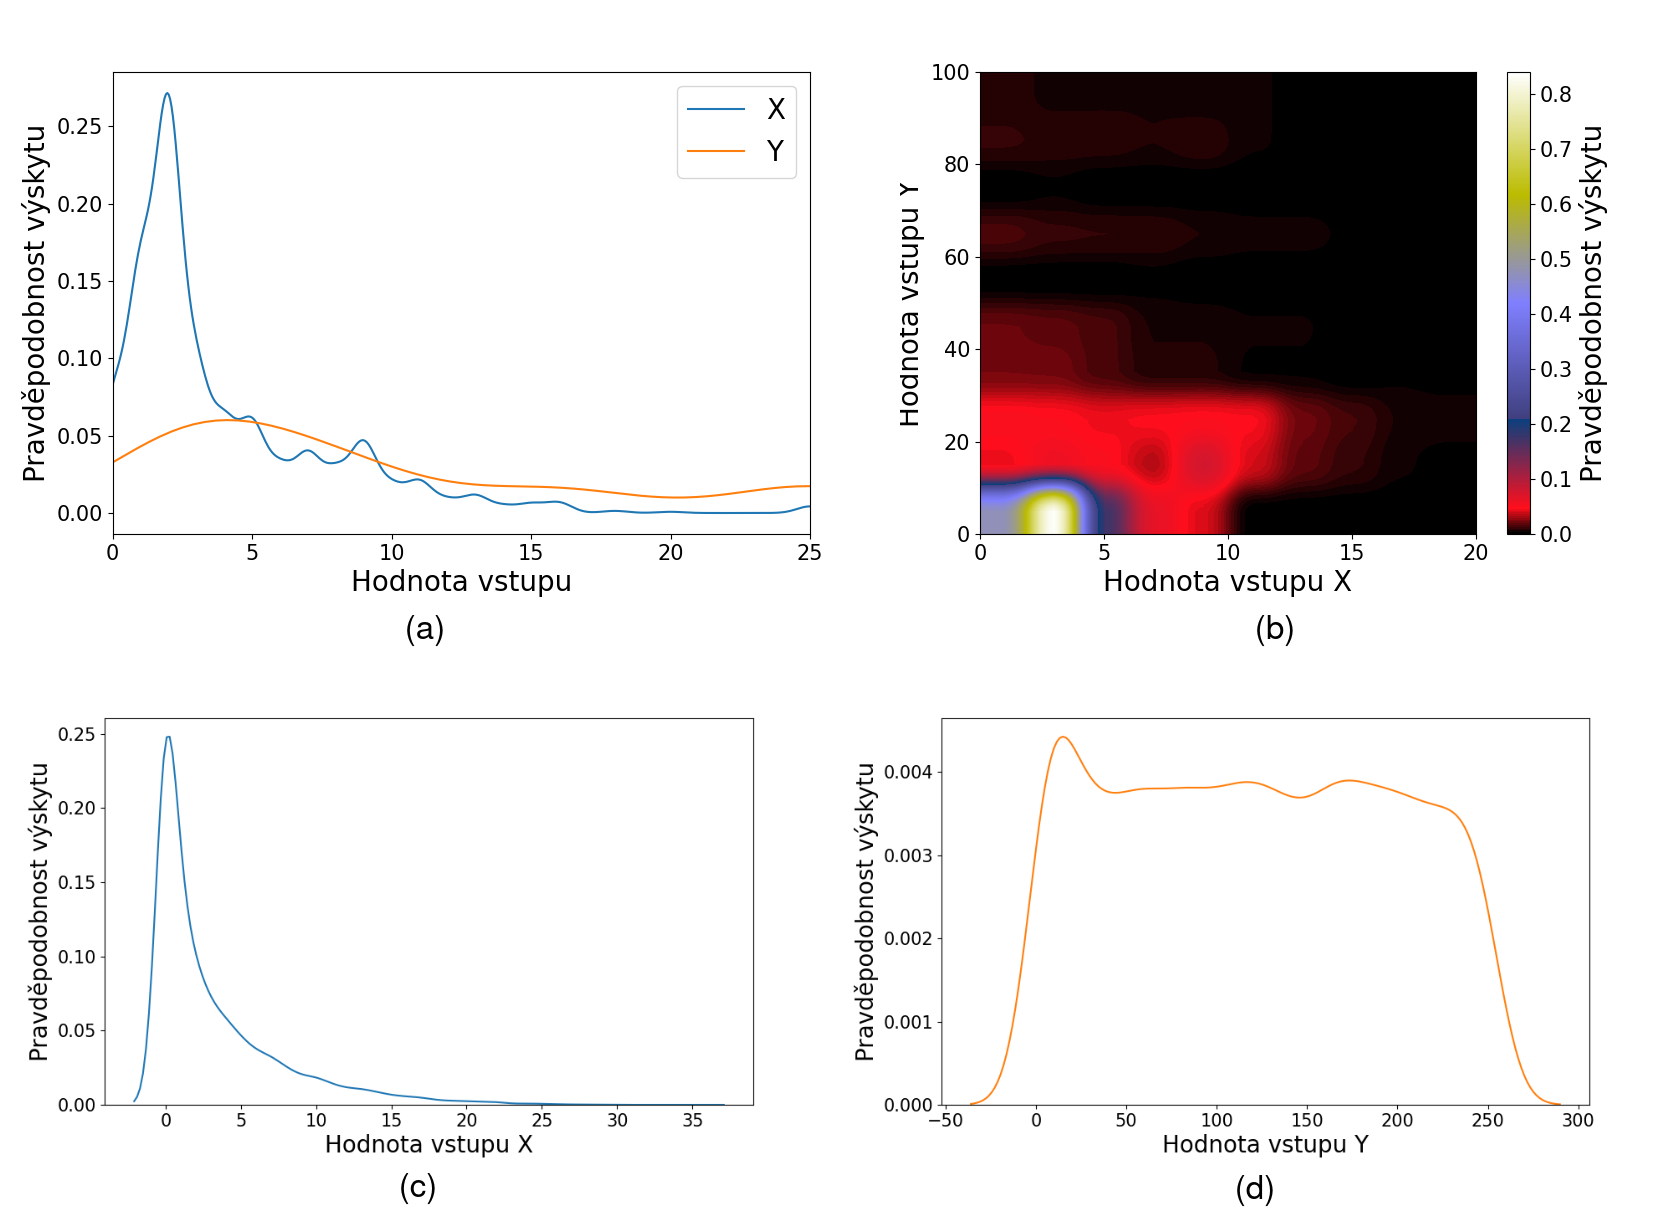
\includegraphics[width=0.85\textwidth]{obrazky-figures/beta_uni_all.png}
    \caption{(a) a (b) PDF násobených dvojic rasterizačního algoritmu Ellipse Mid-Point, (c) a (d) Pravděpodobnostní rozdělení použitá při generování náhodných vstupů}
    \label{fig:beta_uni}
\end{figure}

\pagebreak

\subsubsection{Bresenhamův algoritmus}
Bresenhamův algoritmus je algoritmus používaný v grafice pro rasterizaci úsečky. Na obrázku \ref{fig:const_norm} jsou znázorněna pravděpodobnostní rozdělení vstupů násobičky. Pseudokód zvolených rozdělení je následující:

\begin{lstlisting}[language={C}, label={lst:bresenham}]
input_x = 2

input_y = int(random_normal(150, 30))
if input_y < 0:
    input_y = int(random(100, 255))
\end{lstlisting}

V algoritmu dochází pouze k násobení různých hodnot číslem 2. Vstupem X je tedy konstanta 2, vstup Y přibližně odpovídá normálnímu rozdělení se střední hodnotou 150 a rozptylem 30. V rámci experimentů byl tento způsob generování čísel označen jako \textbf{const\_norm}.

\begin{figure}[H]
    \centering
    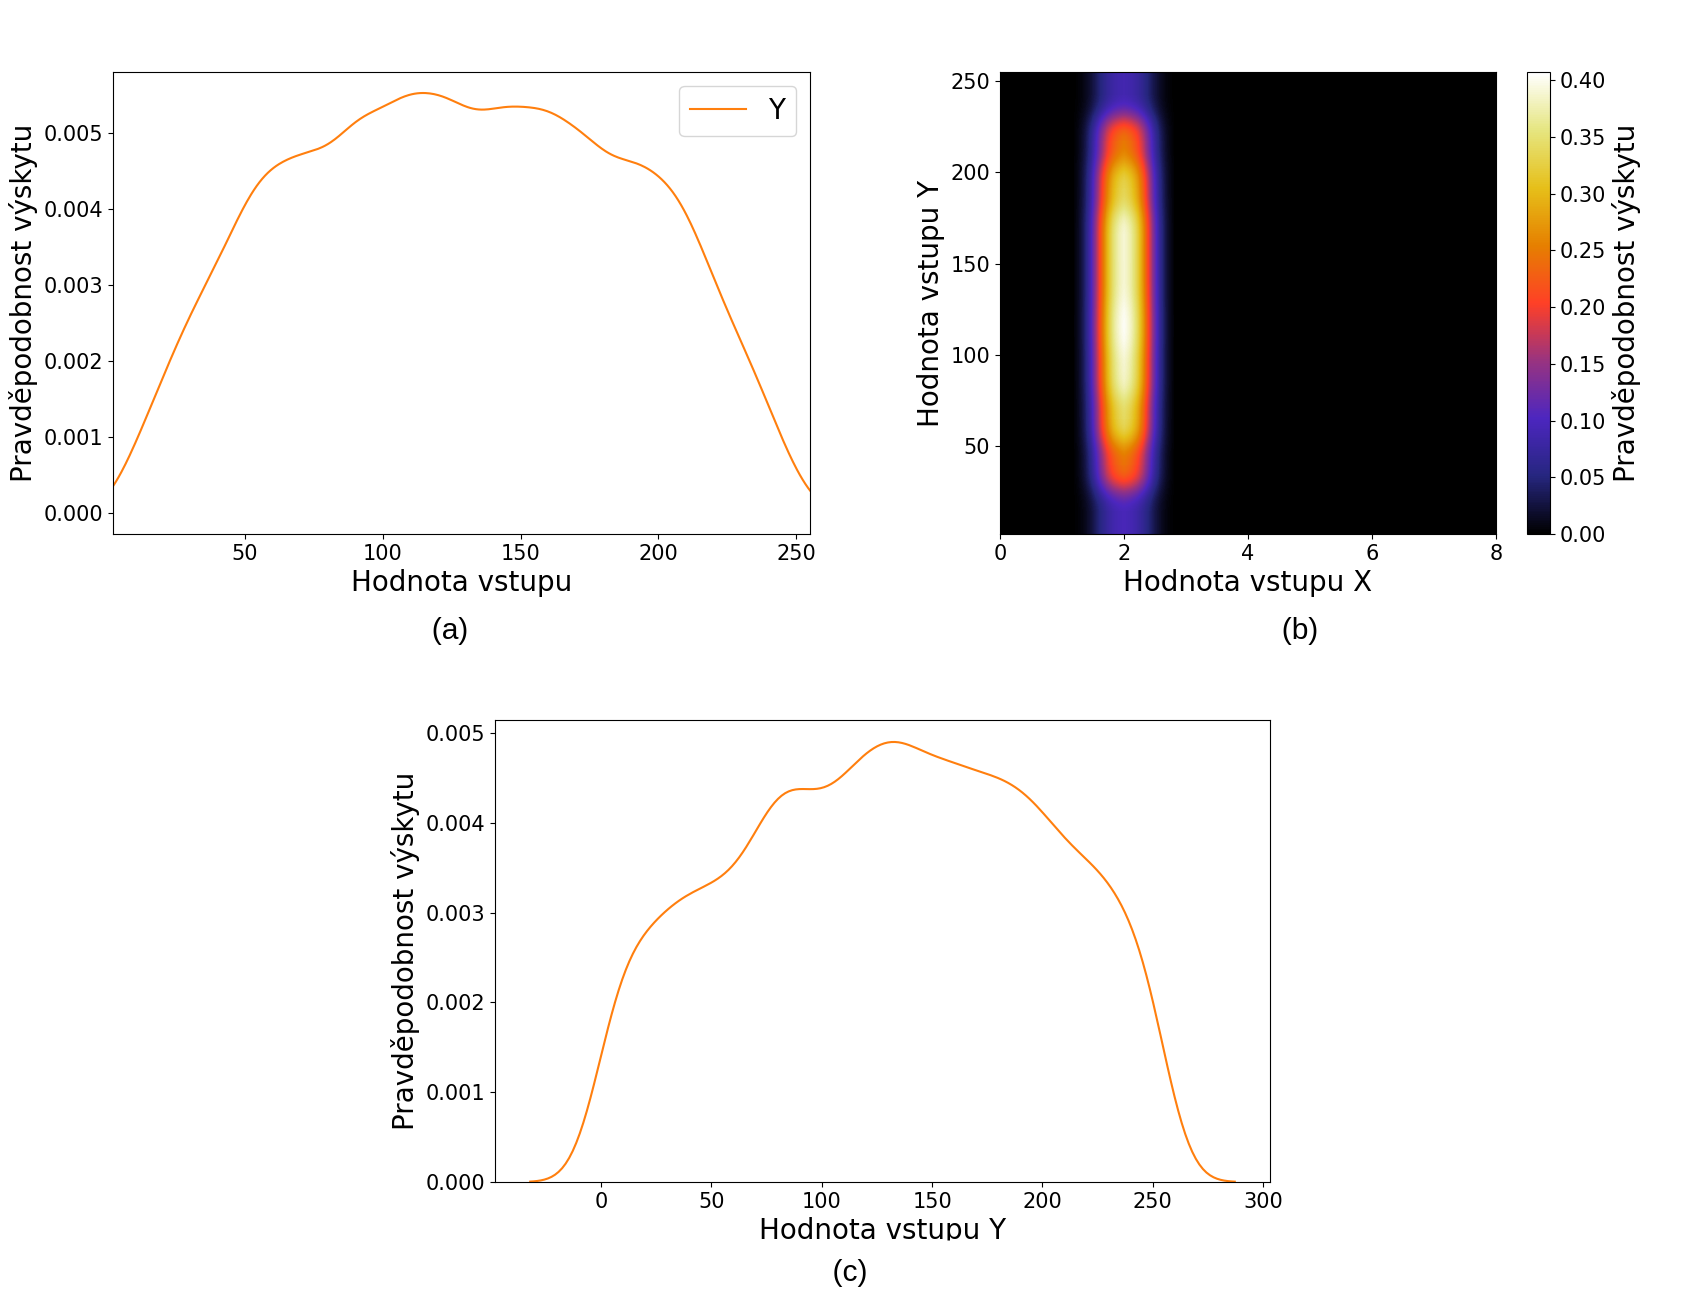
\includegraphics[width=\textwidth]{obrazky-figures/const_norm_all.png}
    \caption{(a) a (b) PDF násobených dvojic Bresenhamova rasterizačního algoritmu, (c) Pravděpodobnostní rozdělení použité při generování náhodných vstupů}
    \label{fig:const_norm}
\end{figure}

\pagebreak

\subsubsection{Pritchardovo síto}
Pritchardovo síto (angl. \textit{Sieve of Pritchard}) je algoritmus z oblasti teorie čísel používaný pro nalezení všech prvočísel menších než je daná hranice. Na obrázku \ref{fig:gamma_2norm} jsou znázorněna pravděpodobnostní rozdělení vstupů násobičky. Pseudokód zvolených rozdělení je následující:

\begin{lstlisting}[language={C}, label={lst:pritchard}]
input_x = int(random_gamma(1.0, 0.8) * 7)

input_y = int(random_uniform(0, 256))
if 100 < input_y < 175:
    input_y = int(random_uniform(0, 75))

if 175 <= input_y < 200:
    input_y = int(random_uniform(200, 255))
\end{lstlisting}

Pro generování vstupu X bylo zvoleno rozdělení gamma s parametry $k = 1.0$ a $\theta = 0.8$ následně vynásobené hodnotou 7. Vstup Y byl generován kombinací několika rovnoměrných rozdělení, což dalo vzniknout dvěma přibližným normálním rozdělením okolo středů 50 a 220. V rámci experimentů byl tento způsob generování čísel označen jako \textbf{gamma\_2norm}.

\begin{figure}[H]
    \centering
    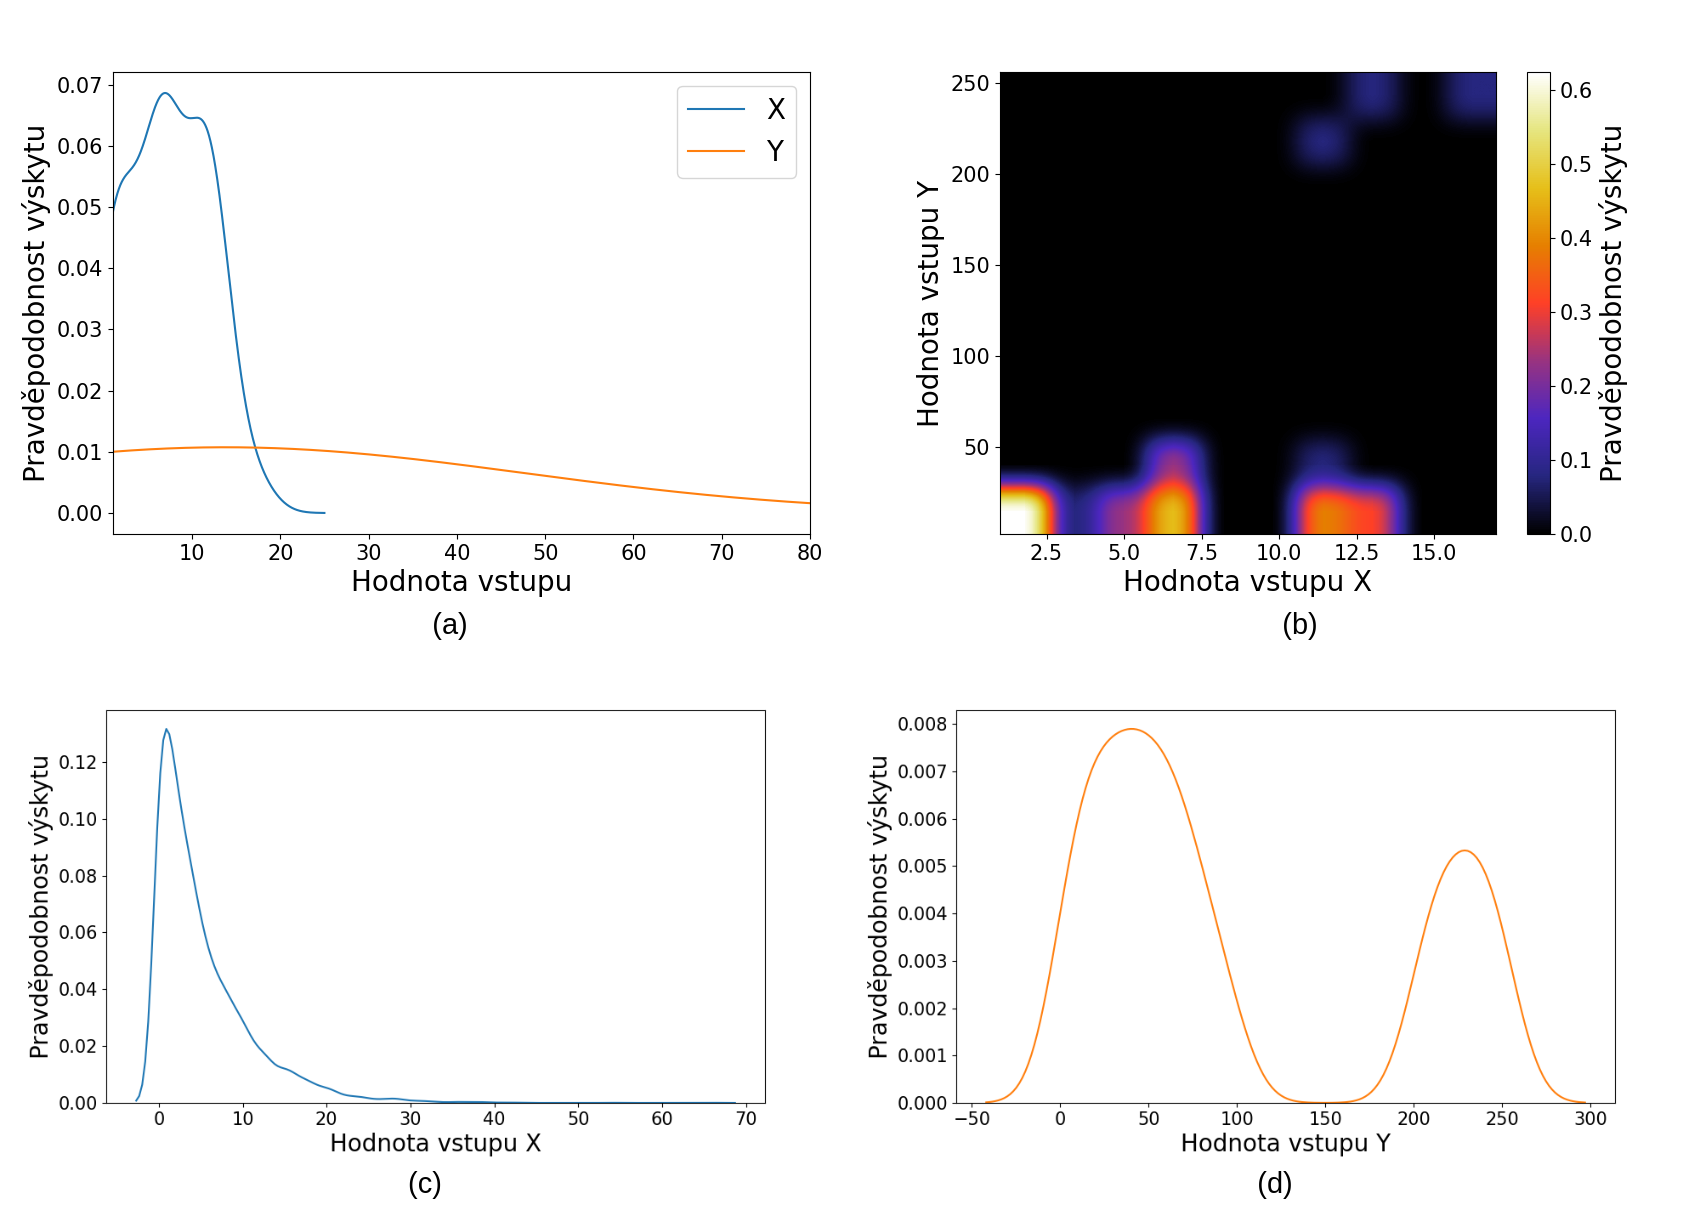
\includegraphics[width=\textwidth]{obrazky-figures/gamma_2norm_all.png}
    \caption{(a) a (b) PDF násobených dvojic v algoritmu Pritchardovo síto, (c) a (d) Pravděpodobnostní rozdělení použitá při generování náhodných vstupů}
    \label{fig:gamma_2norm}
\end{figure}

\pagebreak

\subsubsection{Algoritmus Integer Square Root}
Algoritmus používaný k určení celočíselné odmocniny nějakého čísla, tedy největšího přirozeného čísla, které je menší nebo rovno odmocnině daného čísla. Na obrázku \ref{fig:same_triang} jsou znázorněna pravděpodobnostní rozdělení vstupů násobičky. Pseudokód zvolených rozdělení je následující:

\begin{lstlisting}[language={C}, label={lst:isqrt}]
input_x = int(random_triangular(-10, 255, 10))

input_y = input_x
\end{lstlisting}

V algoritmu dochází k umocňování na druhou, oba vstupy jsou tedy stejná čísla. Frekventovanější jsou menší hodnoty, proto bylo pro generování zvoleno triangulární rozdělení s minimem v -10, maximem v 255 a modem v hodnotě 10. V rámci experimentů byl tento způsob generování čísel označen jako \textbf{same\_triang}.

\begin{figure}[H]
    \centering
    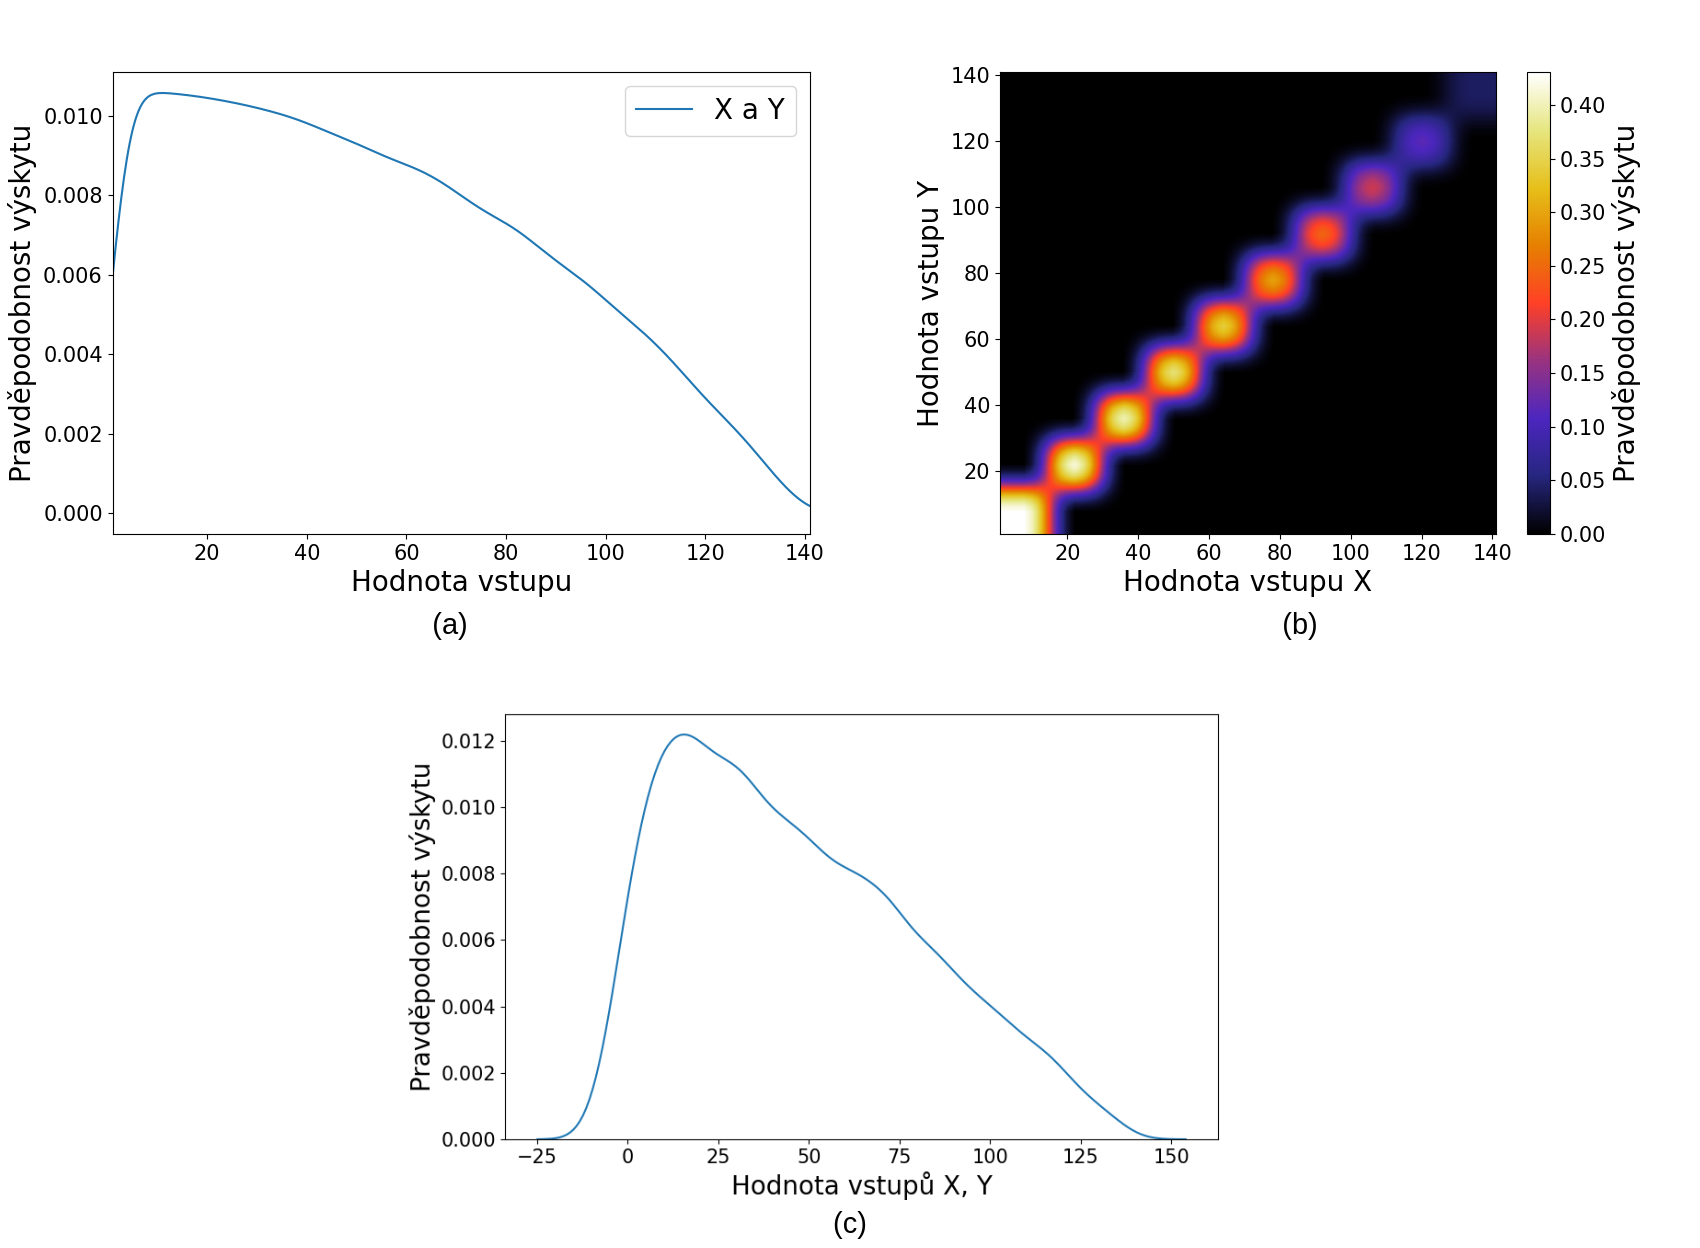
\includegraphics[width=\textwidth]{obrazky-figures/same_triang_all.png}
    \caption{(a) a (b) PDF násobených dvojic v algoritmu výpočtu celočíselné odmocniny, (c) Pravděpodobnostní rozdělení použité při generování náhodných vstupů}
    \label{fig:same_triang}
\end{figure}

\pagebreak

\subsubsection{Algoritmus Circle Point to Point}
Algoritmus používaný v grafice k rasterizaci kružnice. Na obrázku \ref{fig:same_uni} jsou znázorněna pravděpodobnostní rozdělení vstupů násobičky. Pseudokód zvolených rozdělení je následující:

\begin{lstlisting}[language={C}, label={lst:circle}]
input_x = int(random_uniform(0, 255))

input_y = input_x
\end{lstlisting}

V algoritmu Point to Point dochází, podobně jako u předchozího algoritmu, k umocňování čísel na druhou. V tomto případě ovšem vstupy následují přibližně rovnoměrné rozdělení od 0 do 255. V rámci experimentů byl tento způsob generování čísel označen jako \textbf{same\_uni}.

\begin{figure}[H]
    \centering
    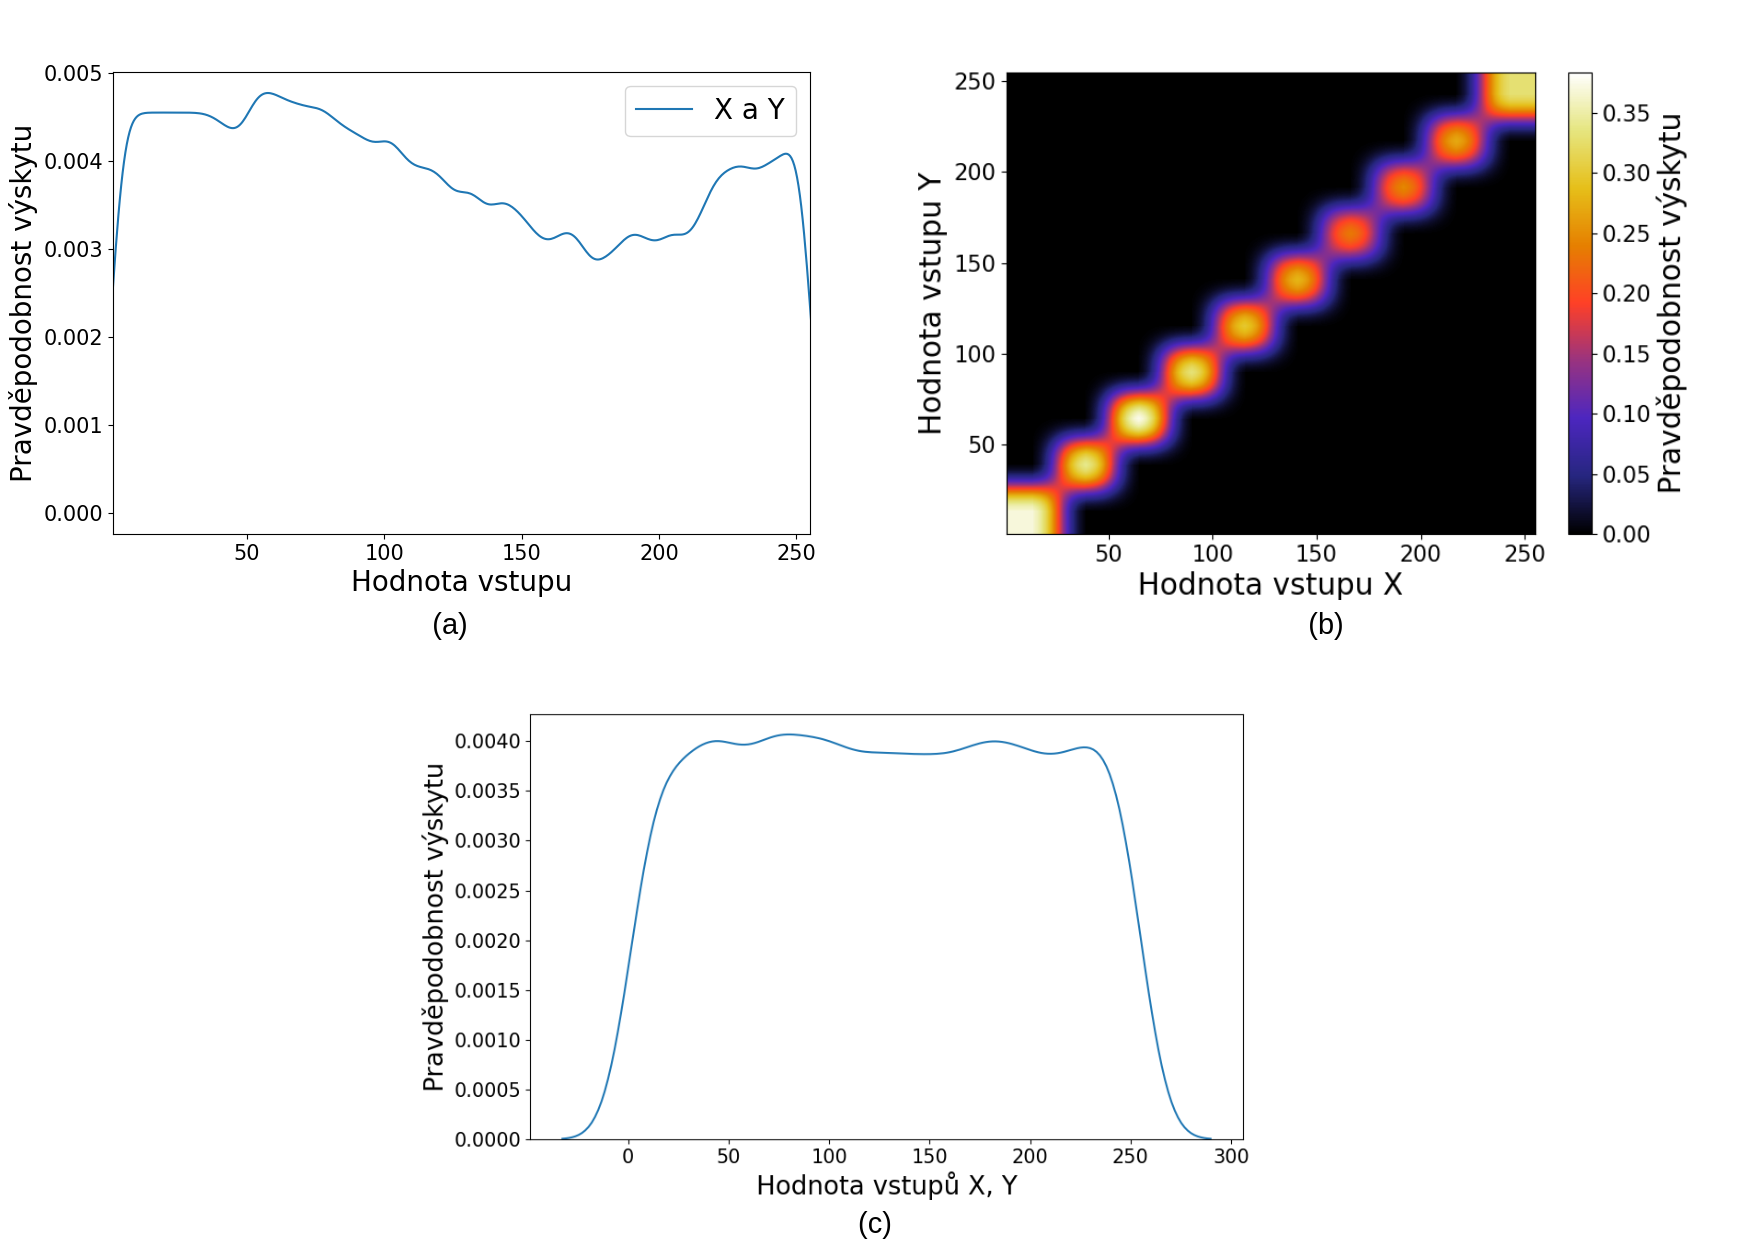
\includegraphics[width=\textwidth]{obrazky-figures/same_uni.png}
    \caption{(a) a (b) PDF násobených dvojic v algoritmu Circle Point to Point, (c) Pravděpodobnostní rozdělení použité při generování náhodných vstupů}
    \label{fig:same_uni}
\end{figure}

\pagebreak

\subsubsection{Algoritmus AKS}
AKS je algoritmus z oblasti teorie čísel sloužící k ověření toho, zda je nějaké dané číslo prvočíslem. Na obrázku \ref{fig:triang_beta} jsou znázorněna pravděpodobnostní rozdělení vstupů násobičky. Pseudokód zvolených rozdělení je následující:

\begin{lstlisting}[language={C}, label={lst:aks}]
input_x = int(random_triangular(-50, 450, 70))
if input_x > 255:
    input_x = int(random_uniform(0, 150))

input_y = fint(random_beta(2.0, 2.0) * 255);
\end{lstlisting}

Rozdělení vstupu X přibližně odpovídá triangulárnímu rozdělení s minimem -50, maximem 450 a modem v hodnotě 70. Vstup Y byl generován podle rozdělení beta s parametry $\alpha = 2$ a $\beta = 2$. Vygenerovaná hodnota byla následně vynásobena 255 (beta rozdělení figuruje na intervalu 0 až 1). V rámci experimentů byl tento způsob generování čísel označen jako \textbf{triang\_beta}.

\begin{figure}[H]
    \centering
    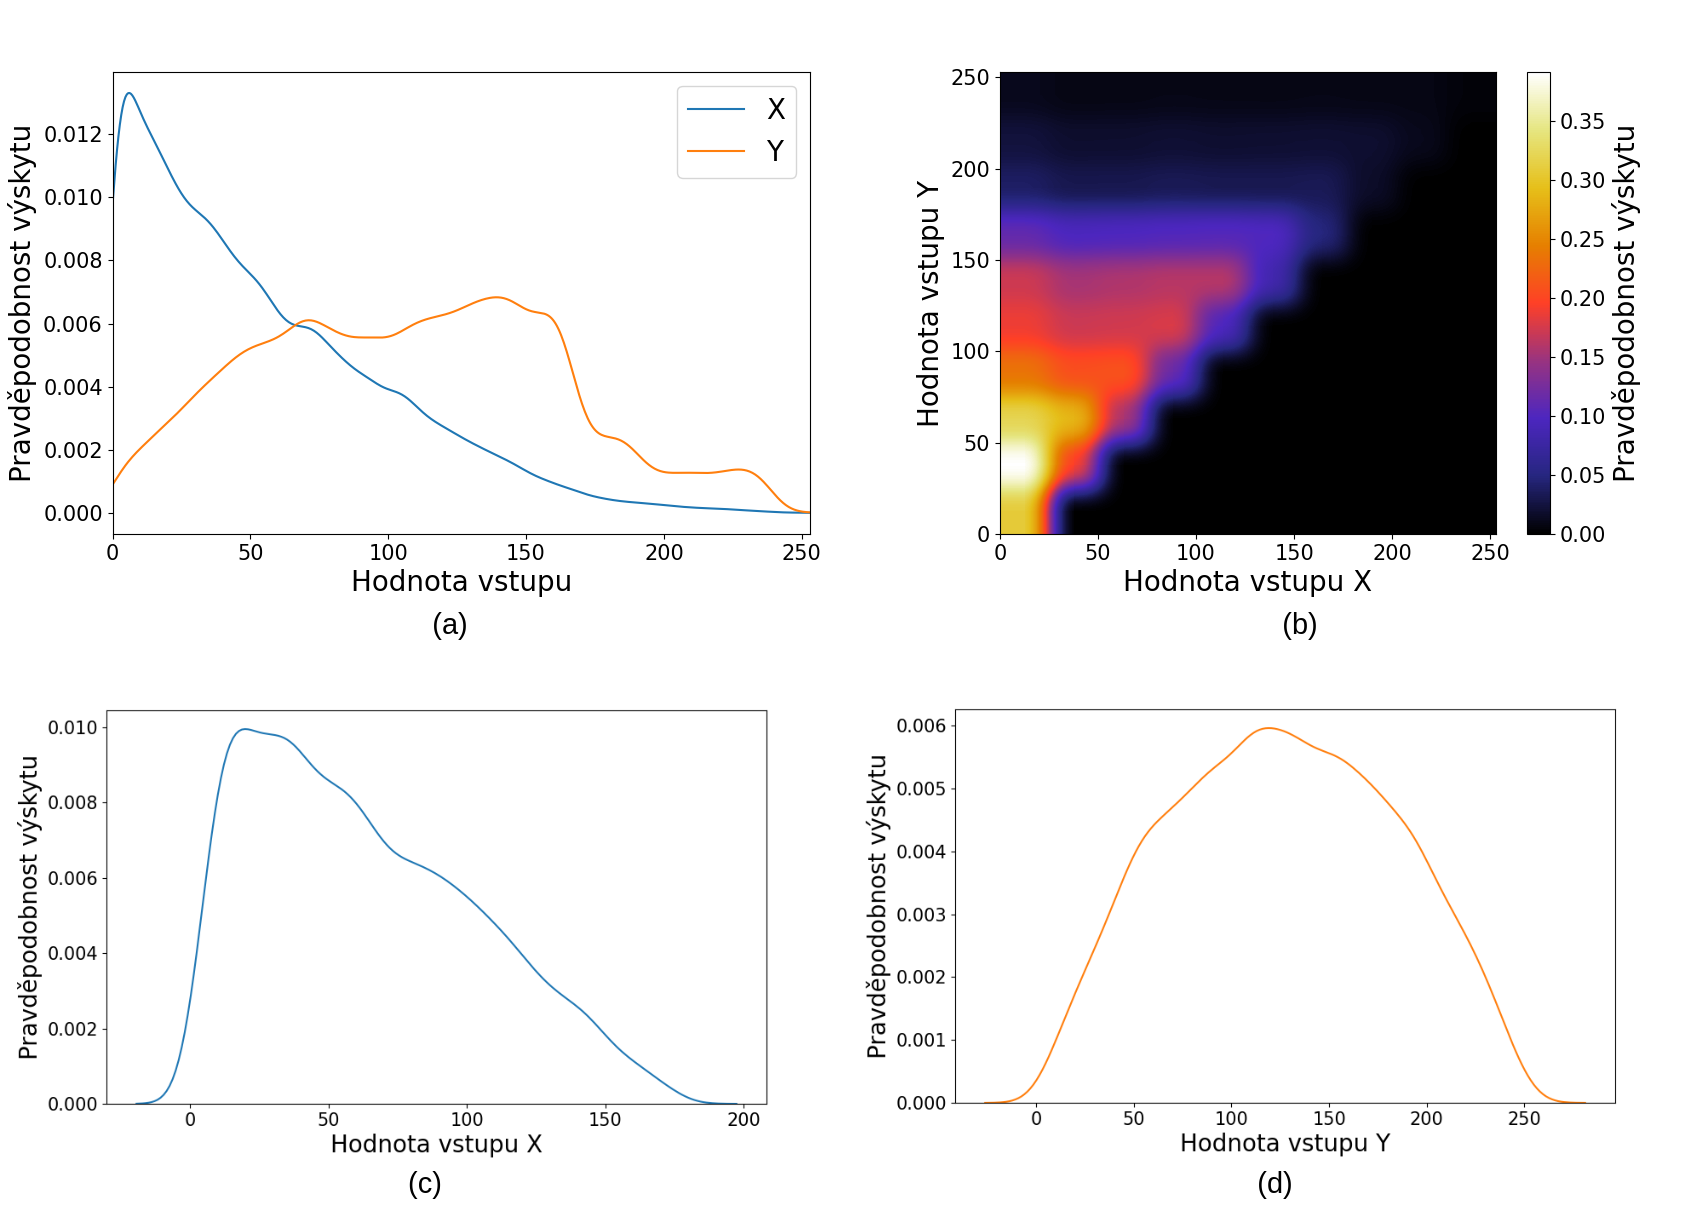
\includegraphics[width=\textwidth]{obrazky-figures/triang_beta_all.png}
    \caption{(a) a (b) PDF násobených dvojic v algoritmu AKS, (c) a (d) Pravděpodobnostní rozdělení použitá při generování náhodných vstupů}
    \label{fig:triang_beta}
\end{figure}

\pagebreak

\subsubsection{Algoritmus ElGamal}
Algoritmus ElGamal slouží k asymetrickému šifrování klíčů. Na obrázku \ref{fig:triang_weibull} jsou znázorněna pravděpodobnostní rozdělení vstupů násobičky. Pseudokód zvolených rozdělení je následující:

\begin{lstlisting}[language={C}, label={lst:elgamal}]
input_x = int(random_triangular(0, 350, 0))
if input_x > 255:
    input_x = int(random_uniform(0, 50))

input_y = int(random_weibull(1.7, 1.7) * 60)
if input_y > 255:
    input_y = int(random_uniform(0, 25))
\end{lstlisting}

Vstup X je generován dle lehce deformovaného triangulárního rozdělení s minimem a modem 0 a maximem 350. Hodnoty větší než 350 jsou ovšem zahozeny a je místo nich vygenerováno číslo z intervalu 0 až 50, čímž dochází ke zmíněné deformaci.

Vstup Y je generován pomocí Weibullova rozdělení s parametry $k = 1,7$ a $\lambda = 1,7$ deformovaného podobným způsobem jako vstup X. V rámci experimentů byl tento způsob generování čísel označen jako \textbf{triang\_weibull}.

\begin{figure}[H]
    \centering
    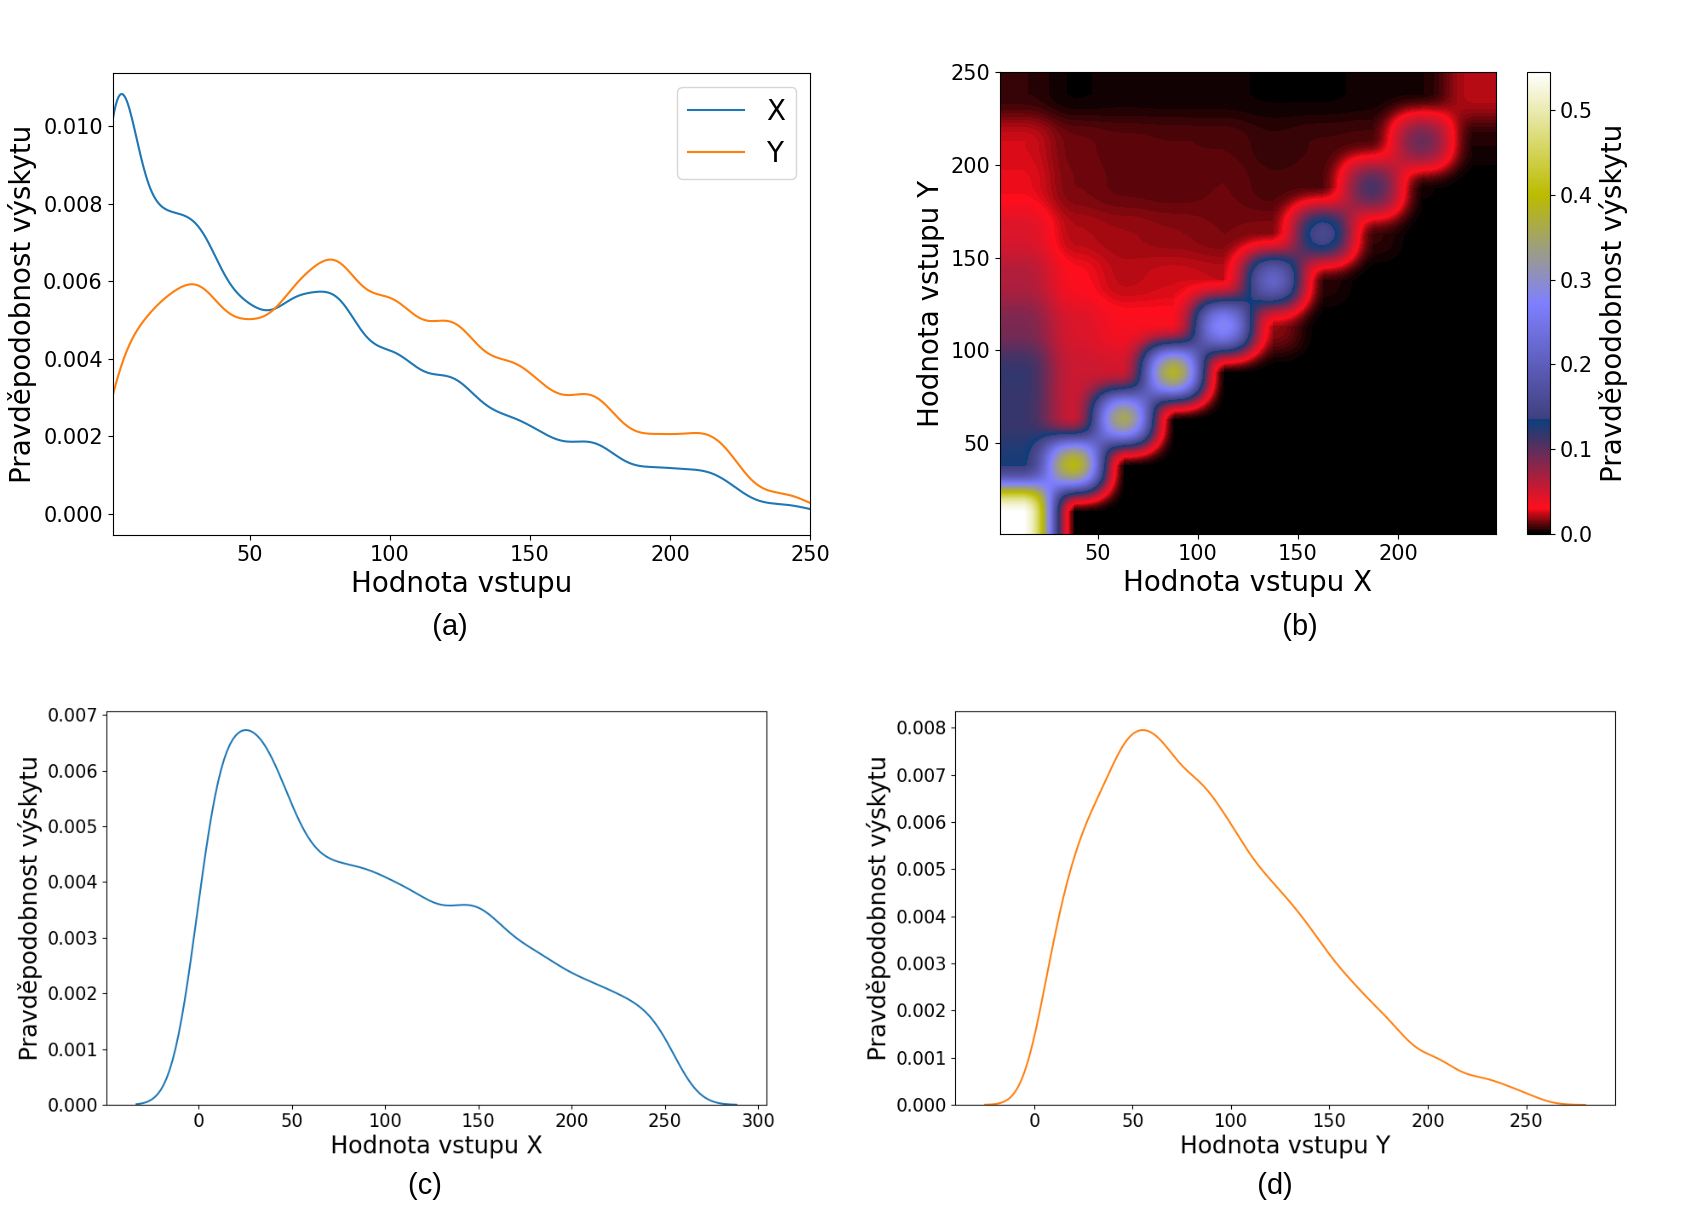
\includegraphics[width=\textwidth]{obrazky-figures/triang_weibull_all.png}
    \caption{(a) a (b) PDF násobených dvojic v algoritmu ElGamal, (c) a (d) Pravděpodobnostní rozdělení použitá při generování náhodných vstupů}
    \label{fig:triang_weibull}
\end{figure}

\section{Simulační dotazy} \label{sim_dotazy}
Pro simulaci chování násobiček bylo v systému UPPAAL vytvořeno několik dotazů.

První z nich slouží k ověření, že se správně generují vstupní hodnoty. Zároveň může čtenáři sloužit k upřesnění představy o tom, jaké vstupy se generují v rámci jednotlivých rozdělení. Výstupem je graf znázorňující hodnoty vstupních čísel v jednotlivých časových okamžicích. 

Jeden příklad výstupu lze pozorovat na obrázku \ref{fig:input_sim_example}, příklady pro všechny typy použitých rozdělení jsou poté uvedeny v příloze \ref{append:control_sims} v části \textbf{Kontrola vstupních hodnot}. Dotaz vypadá následovně:

\begin{equation*}
    \texttt{simulate[<=20000;1] {input\_a, input\_b}}
\end{equation*}

\begin{figure}[H]
    \centering
    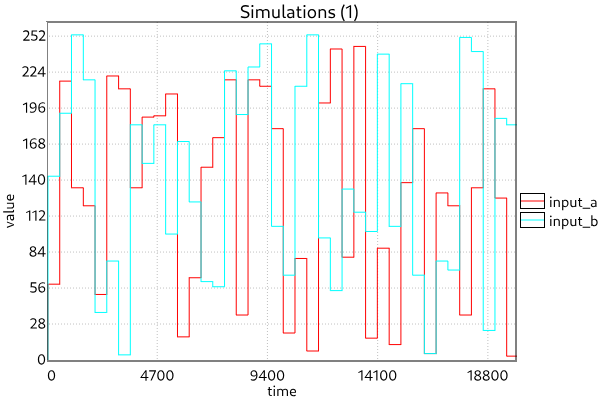
\includegraphics[width=0.6\textwidth]{obrazky-figures/inputs_uni_uni.png}
    \caption{Příklad výstupu dotazu ověřujícího hodnoty vygenerovaných vstupů}
    \label{fig:input_sim_example}
\end{figure}

Druhý dotaz slouží k porovnání výstupů přesné a zkoumané přibližné násobičky. Podobně jako u předchozího dotazu je výstupem graf zobrazující obě hodnoty v jednotlivých časových okamžicích. Příklady výstupů pro násobičky s různou úrovní aproximace lze pozorovat v příloze \ref{append:control_sims} v části \textbf{Porovnání přesných a přibližných výstupů}. Dotaz má následující podobu:

\begin{equation*}
    \texttt{simulate[<=20000;1] {res\_acc, res\_approx}}
\end{equation*}

Třetí dotaz zobrazuje zpoždění, které zkoumaná násobička nabírá při jednotlivých výpočtech. To může sloužit jednak k porovnání zpoždění jednotlivých násobiček, dále lze z grafů i vypozorovat, kolika dílčími hradly daný výpočet prochází. Příklady výstupů pro méně přesnou a velmi přesnou aproximační násobičku lze pozorovat v příloze \ref{append:control_sims} v části \textbf{Sledování zpoždění}. Dotaz vypadá následovně:

\begin{equation*}
    \texttt{simulate[<=1000;1] {current\_delay}}
\end{equation*}

\pagebreak

Čtvrtý dotaz tvoří hlavní část experimentů. V rámci tohoto dotazu jsou sledovány všechny vybrané hodnotící metriky. Dotaz má následující podobu:

\begin{equation*}
    \begin{array}{l}
        \texttt{simulate[<=10000000;1] \{coverage\_percentage, delay\_avg, error\_prob,} \\
        \texttt{    mean\_abs\_error, mean\_relative\_error, mean\_squared\_error,} \\
        \texttt{    avg\_flips\_per\_res, worst\_case\_error, worst\_case\_relative\_error,} \\
        \texttt{    max\_hamming\_distance, max\_bit\_flips, worst\_delay\}}
    \end{array}
\end{equation*}

Jednotlivé sledované proměnné mají následující význam:

\begin{itemize}
    \item \texttt{coverage\_percentage} -- procento pokrytí všech kombinací vstupů,
    \item \texttt{delay\_avg} -- průměrné zpoždění jednoho výpočtu přibližné násobičky,
    \item \texttt{error\_prob} -- pravděpodobnost chyby,
    \item \texttt{mean\_abs\_error} -- průměrná absolutní chyba,
    \item \texttt{mean\_relative\_error} -- průměrná relativní chyba,
    \item \texttt{mean\_squared\_error} -- průměrná kvadratická chyba,
    \item \texttt{avg\_flips\_per\_res} -- průměrný počet překlopených bitů v logických hradlech v rámci jednoho výpočtu,
    \item \texttt{worst\_case\_error} -- nejhorší absolutní chyba,
    \item \texttt{worst\_case\_relative\_error} -- nejhorší relativní chyba,
    \item \texttt{max\_hamming\_distance} -- maximální Hammingova vzdálenost mezi výsledky přesné a přibližné násobičky,
    \item \texttt{max\_bit\_flips} -- maximální počet překlopených bitů v logických hradlech v rámci jednoho výpočtu,
    \item \texttt{worst\_delay} -- nejhorší zpoždění jednoho výpočtu přibližné násobičky.
\end{itemize}

Většina těchto metrik byla již popsána v sekci \ref{error_metrics}. Překlopení bitu logického hradla je situace, v níž se výstupní bit daného hradla po výpočtu nastaví na opačnou hodnotu, než jakou měl před výpočtem. Jedná se o metriku, kterou lze dále využít k výpočtu energetické spotřeby obvodu.

Doba trvání běhu 10 000 000 časových jednotek byla určena experimentálně. Za tuto dobu je systém schopen pokrýt přibližně čtvrtinu všech vstupních kombinací (u referenčního rozdělení \texttt{uni\_uni}), což zajišťuje dostatečně přesné výsledky ve srovnání s referenční knihovnou EvoApproxLib.

Výstupem simulace je soubor ve formátu csv, ze kterého jsou pomocí skriptu \\\texttt{process\_results.py} extrahována veškerá relevantní data. Ta jsou poté uložena do struktury Pandas Dataframe a do tzv. \textit{pickle} souboru (soubor s příponou .pkl vytvořený modulem pickle).

Alternativním způsobem řešení by mohly být dotazy typu
\begin{equation*}
    \texttt{E[<=10000000; 1] (max: error\_prob)},
\end{equation*}
které by byly volány pro každou metriku zvlášť. Tím by se ovšem značně zvýšila časová náročnost simulací (pro každou násobičku v řádech desítek minut až jednotek hodin, v závislosti na výkonu počítače a také na počtu hradel dané násobičky).

\chapter{Výsledky experimentů}
\label{experimenty}
Z knihovny EvoApproxLib bylo vybráno celkem 14 přibližných násobiček 8x8 bitů, na kterých byly prováděny výše popsané simulační dotazy. Při volbě jednotlivých násobiček byla zohledněna jejich plocha a z toho plynoucí úroveň aproximace. Ve vybrané sadě se tak objevují jak násobičky, které jsou sestaveny z méně než 10 logických hradel, tak naopak téměř přesné aproximační násobičky složené z několika stovek logických hradel.

V referenční tabulce \ref{tab:ref_tab} jsou vypsány všechny zvolené násobičky spolu s některými sledovanými metrikami. Údaje o velikosti plochy obvodů byly převzaty z knihovny EvoApproxLib \cite{circuit_library}. Ostatní data pocházejí z výsledků simulací s referenčním rozdělením generovaných vstupů \textbf{uni\_uni}.

\begin{table}[!ht]
    \centering
    \resizebox{0.9\textwidth}{!}{\begin{tabular}{|l|l|l|l|l|}
        \textbf{Násobička} & \textbf{Plocha [$\mu m^2$]} & \Centerstack{\textbf{Pravděpodobnost} \\\textbf{chyby}} & \Centerstack{\textbf{Průměrná} \\\textbf{absolutní chyba}} & \Centerstack{\textbf{Nejhorší} \\\textbf{absolutní chyba}} \\ \hline
        mul8u\_17MN & 13.1 & 0.97 & 2342.61 & 17726 \\ 
        mul8u\_17MJ & 18.8 & 0.89 & 1406.84 & 17030 \\ 
        mul8u\_R36 & 60.5 & 0.98 & 3764.64 & 32289 \\ 
        mul8u\_1A0M & 75.6 & 0.98 & 1796.1 & 7171 \\ 
        mul8u\_Z9D & 220.6 & 0.89 & 3141.56 & 31752 \\ 
        mul8u\_17R6 & 228.5 & 0.98 & 185.57 & 1905 \\ 
        mul8u\_2NDH & 347.8 & 0.99 & 93.52 & 2709 \\ 
        mul8u\_197B & 395.6 & 0.98 & 69.92 & 424 \\ 
        mul8u\_NLX & 511.5 & 0.95 & 6.06 & 161 \\ 
        mul8u\_GTR & 550.5 & 0.84 & 20.1 & 125 \\ 
        mul8u\_BG1 & 561.8 & 0.49 & 289.01 & 2932 \\ 
        mul8u\_R92 & 604.5 & 0.83 & 2.84 & 39 \\ 
        mul8u\_ZB3 & 682.8 & 0.07 & 0.14 & 2 \\ 
        mul8u\_12KA & 683.3 & 0.09 & 11.91 & 192 \\ 
    \end{tabular}}
    \caption{Zkoumané násobičky a vybrané metriky naměřené s rozdělením \texttt{uni\_uni}}
    \label{tab:ref_tab}
\end{table}

V rámci této kapitoly je prezentován výběr z výsledků v podobě sloupcových grafů vždy ve skupinách po čtyřech. Každá skupina se váže k jedné hodnotící metrice, každý graf potom prezentuje výsledky jedné konkrétní násobičky. Jednotlivé sloupce představují různá pravděpodobnostní rozdělení použitá při generování vstupů (viz sekce \ref{rozdeleni_pst}), referenční rozdělení \texttt{uni\_uni} má ve všech grafech šedou barvu. Kompletní výsledky simulací všech násobiček v rámci všech rozdělení jsou k dispozici v příloze \ref{append:exp_results}, každá tabulka se vztahuje k jednomu danému rozdělení.

\pagebreak

\textbf{Pravděpodobnost chyby} u většiny zkoumaných násobiček buď zůstávala podobná, jako u referenčního rozdělení, nebo o něco klesla. K výraznějšímu poklesu pravděpodobnosti chyby docházelo zpravidla u rozdělení, kde alespoň jedno z generovaných čísel nabývá nízkých hodnot (rozdělení \texttt{beta\_uni}, \texttt{const\_norm} a \texttt{gamma\_2norm}). U rozdělení \texttt{const\_norm}, kde je jeden ze vstupů vždy konstanta 2, dokonce některé násobičky generovaly 100 \% přesné výsledky, tedy pravděpodobnost chyby byla nulová. 

Zajimávou anomálií byla násobička \texttt{mul8u\_ZB3}, u které došlo k výraznému zvýšení pravděpodobnosti chyby u rozdělení, která modelovala umocňování čísel na druhou, tedy kde byly oba vstupy stejné (rozdělení \texttt{same\_triang} a \texttt{same\_weibull}). Grafy pravděpodobnosti chyby některých vybraných násobiček lze pozorovat na obrázku \ref{fig:metrics_error_prob}. Bodové grafy v obrázku \ref{fig:scatter_error_prob} potom nabízejí srovnání pravděpodobnosti chyby násobiček v rámci jednotlivých pravděpodobnostních rozdělení.

\begin{figure}[H]
    \centering
    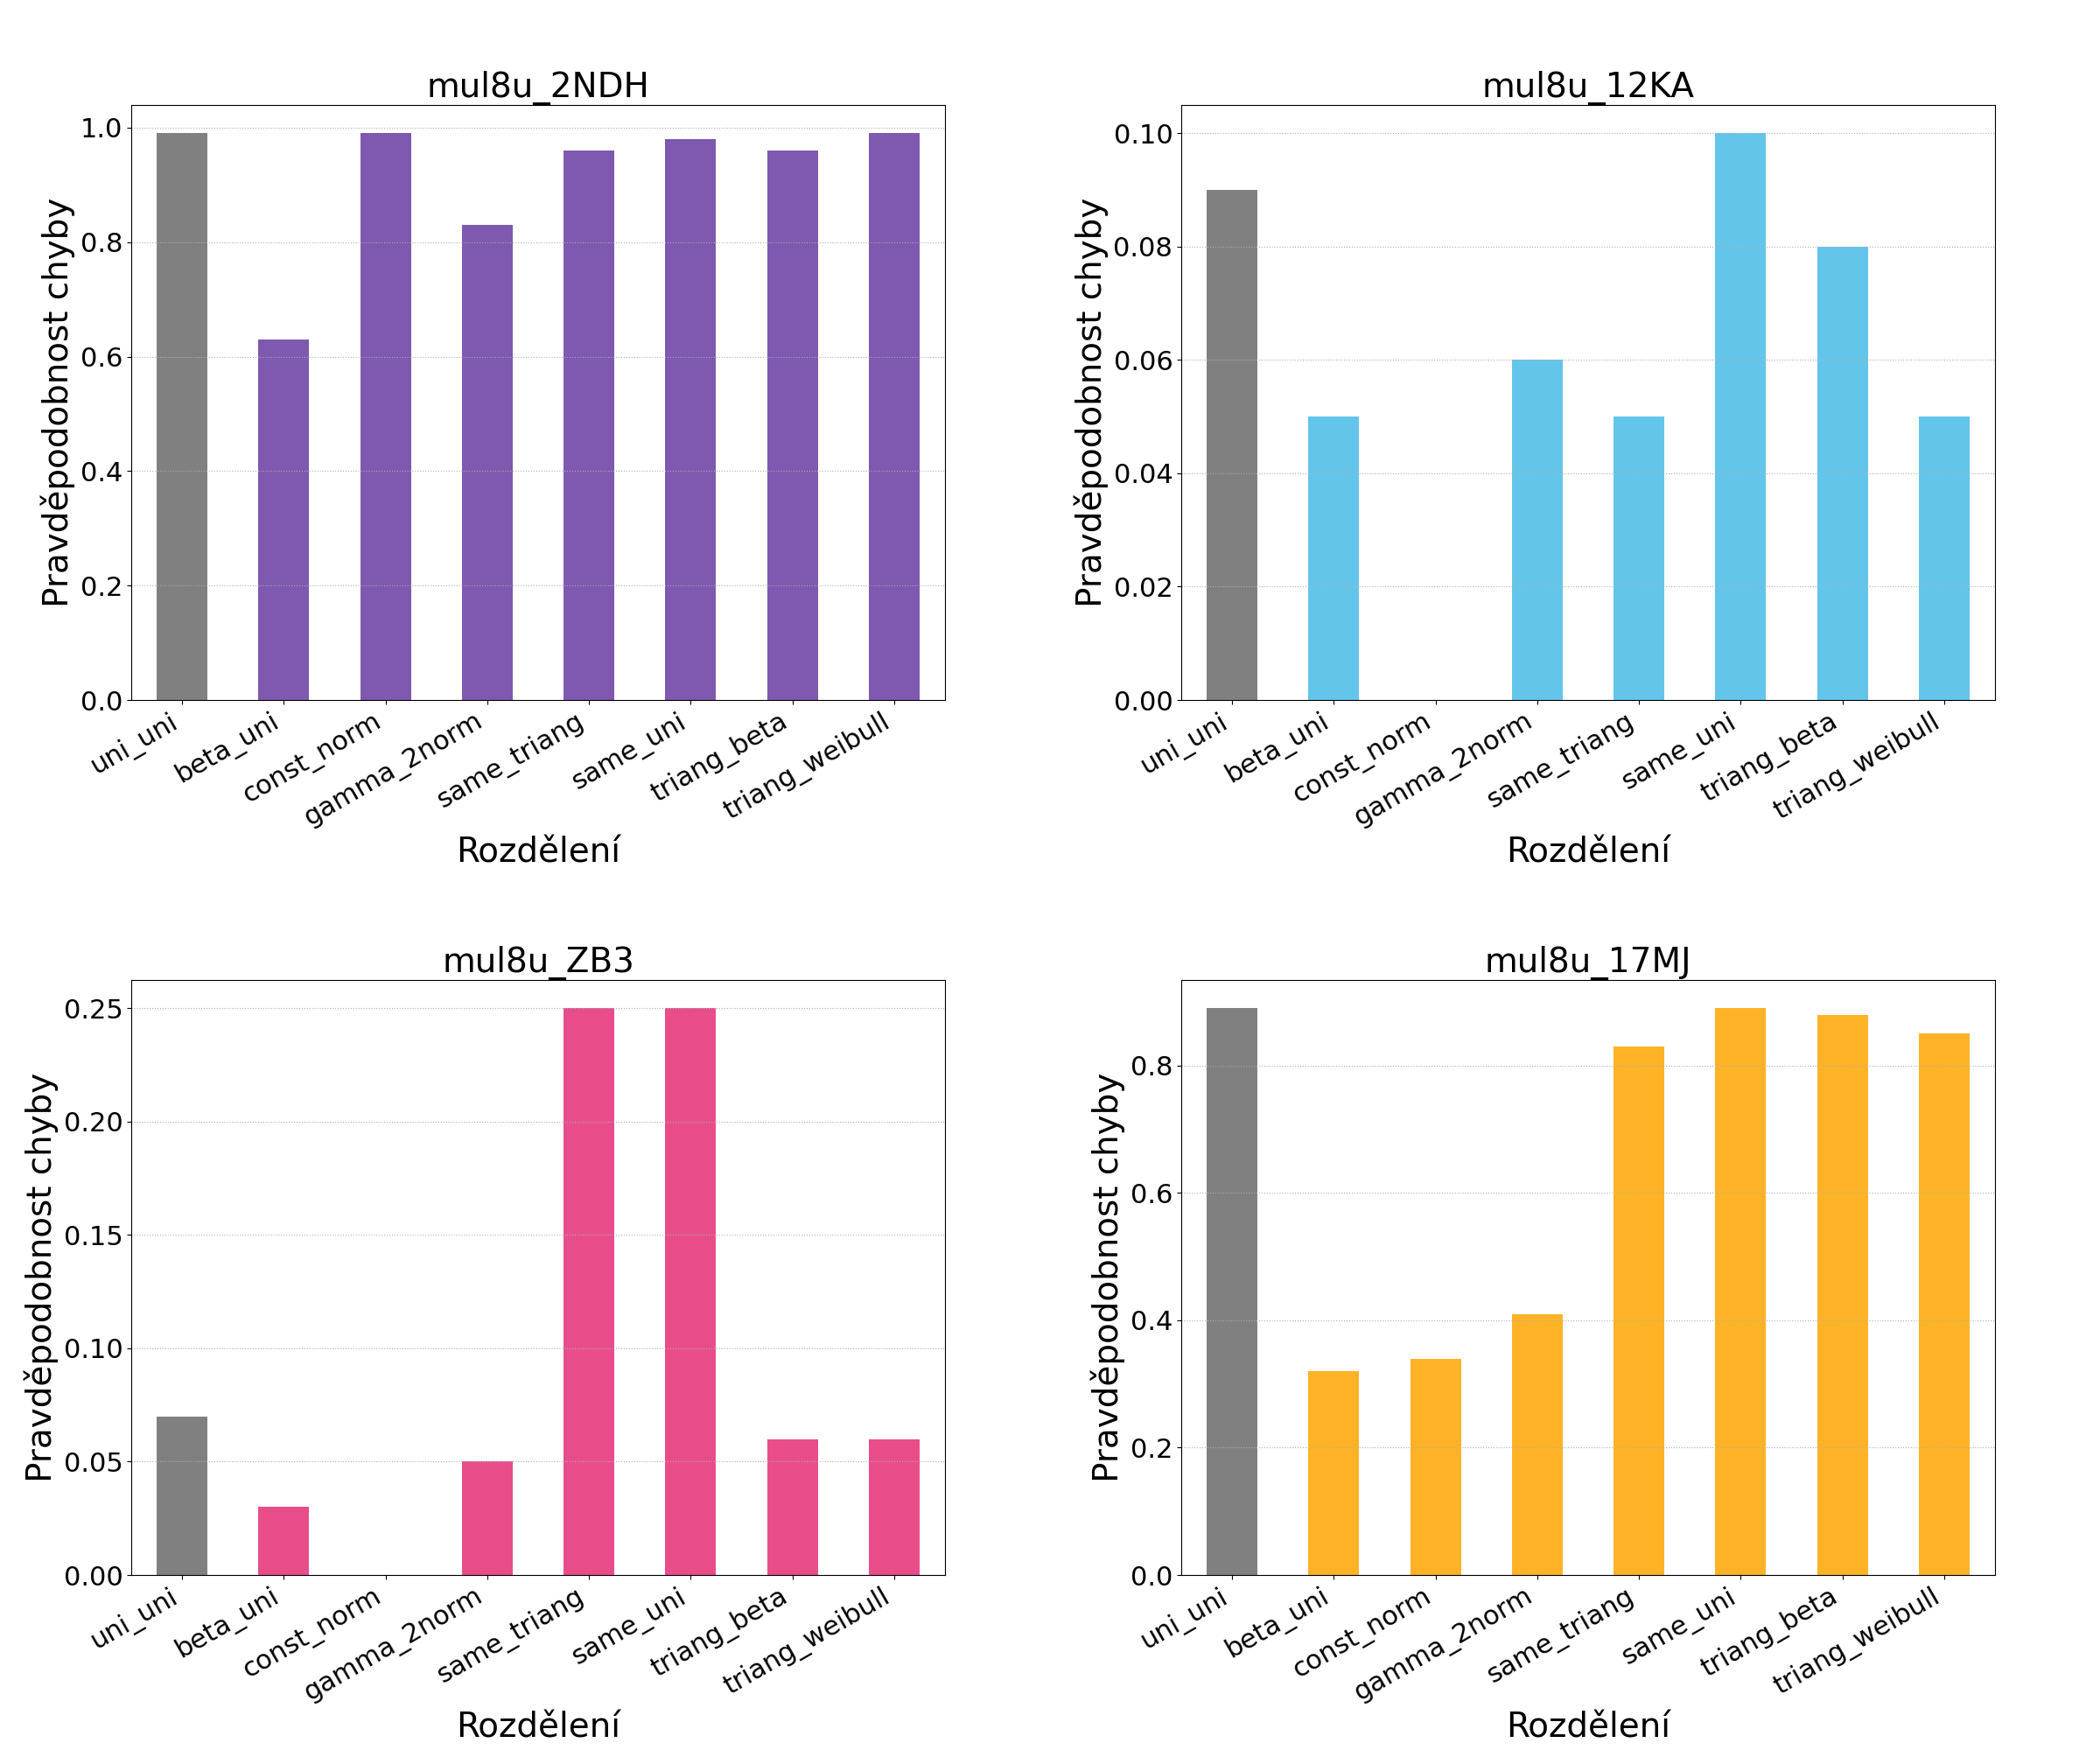
\includegraphics[width=\textwidth]{obrazky-figures/metrics_error_prob.png}
    \caption{Pravděpodobnost chyby vybraných násobiček pro jednotlivá pravděpodobnostní rozdělení vstupních hodnot}
    \label{fig:metrics_error_prob}
\end{figure}

\begin{figure}[H]
    \centering
    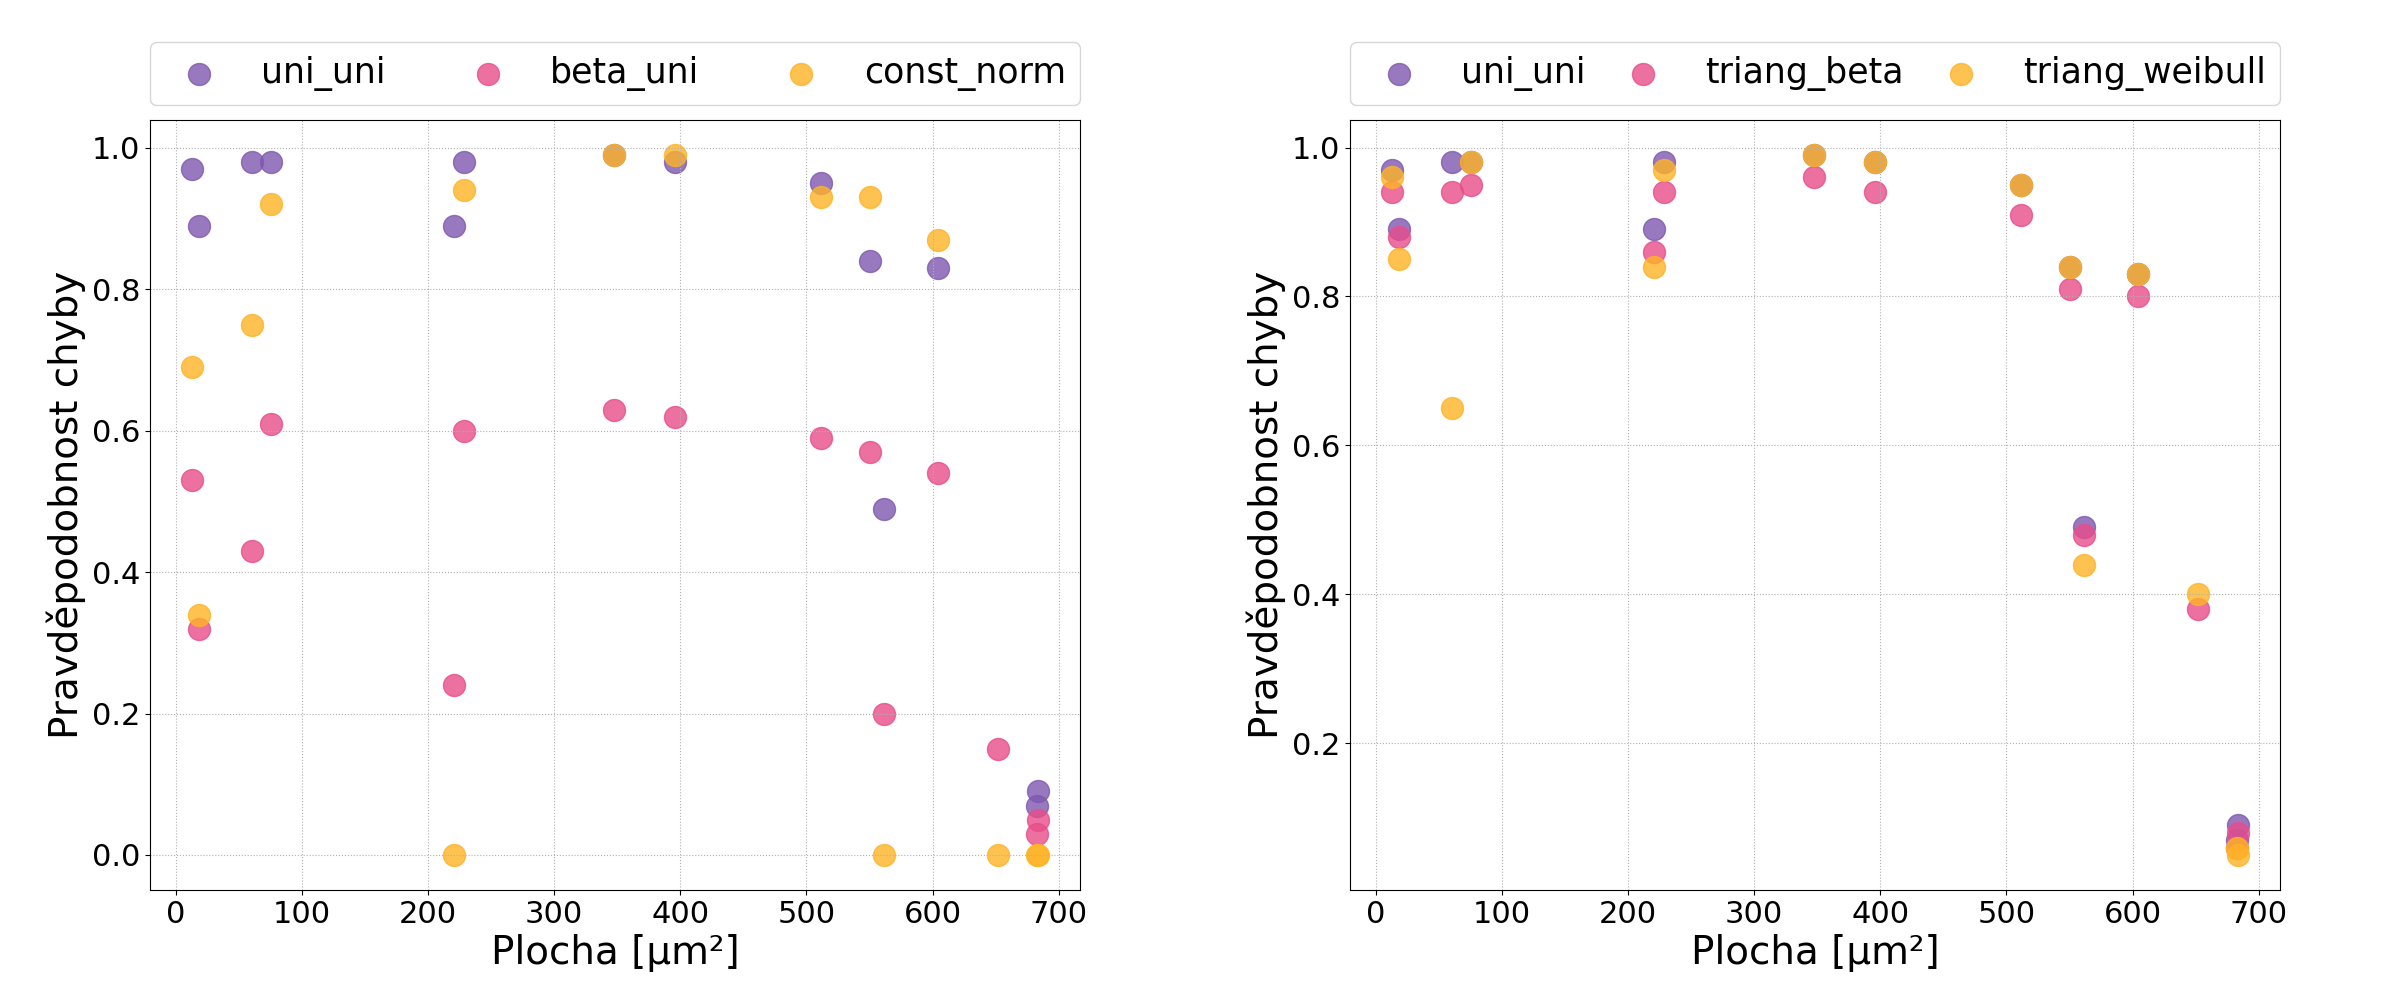
\includegraphics[width=\textwidth]{obrazky-figures/scatter_error_prob.png}
    \caption{Porovnání pravděpodobnosti chyby sledovaných násobiček v rámci vybraných rozdělení}
    \label{fig:scatter_error_prob}
\end{figure}

\textbf{Průměrná absolutní chyba} kolísala v závislosti na úrovni aproximace jednotlivých násobiček. U velmi přesných z nich se naměřené hodnoty pohybovaly nejčastěji v řádech desítek či jednotek (někdy i desetin). Oproti tomu u méně přesných násobiček mnohdy docházelo ke zlepšení (méně často také ke zhoršení) hodnoty průměrné absolutní chyby o několik stovek či tisíc.

Míra zlepšení v rámci jednotlivých pravděpodobnostních rozdělení byla poměrně variabilní. K o něco výraznějším zlepšením opět docházelo u rozdělení generujících menší hodnoty. Výsledky simulací vybraných násobiček jsou vidět v grafech na obrázku \ref{fig:metrics_mean_abs_error}. Obrázek \ref{fig:scatter_mean_abs_error} poté opět slouží k porovnání průměrné absolutní chyby napříč vybranými pravděpodobnostními rozděleními.

\begin{figure}[H]
    \centering
    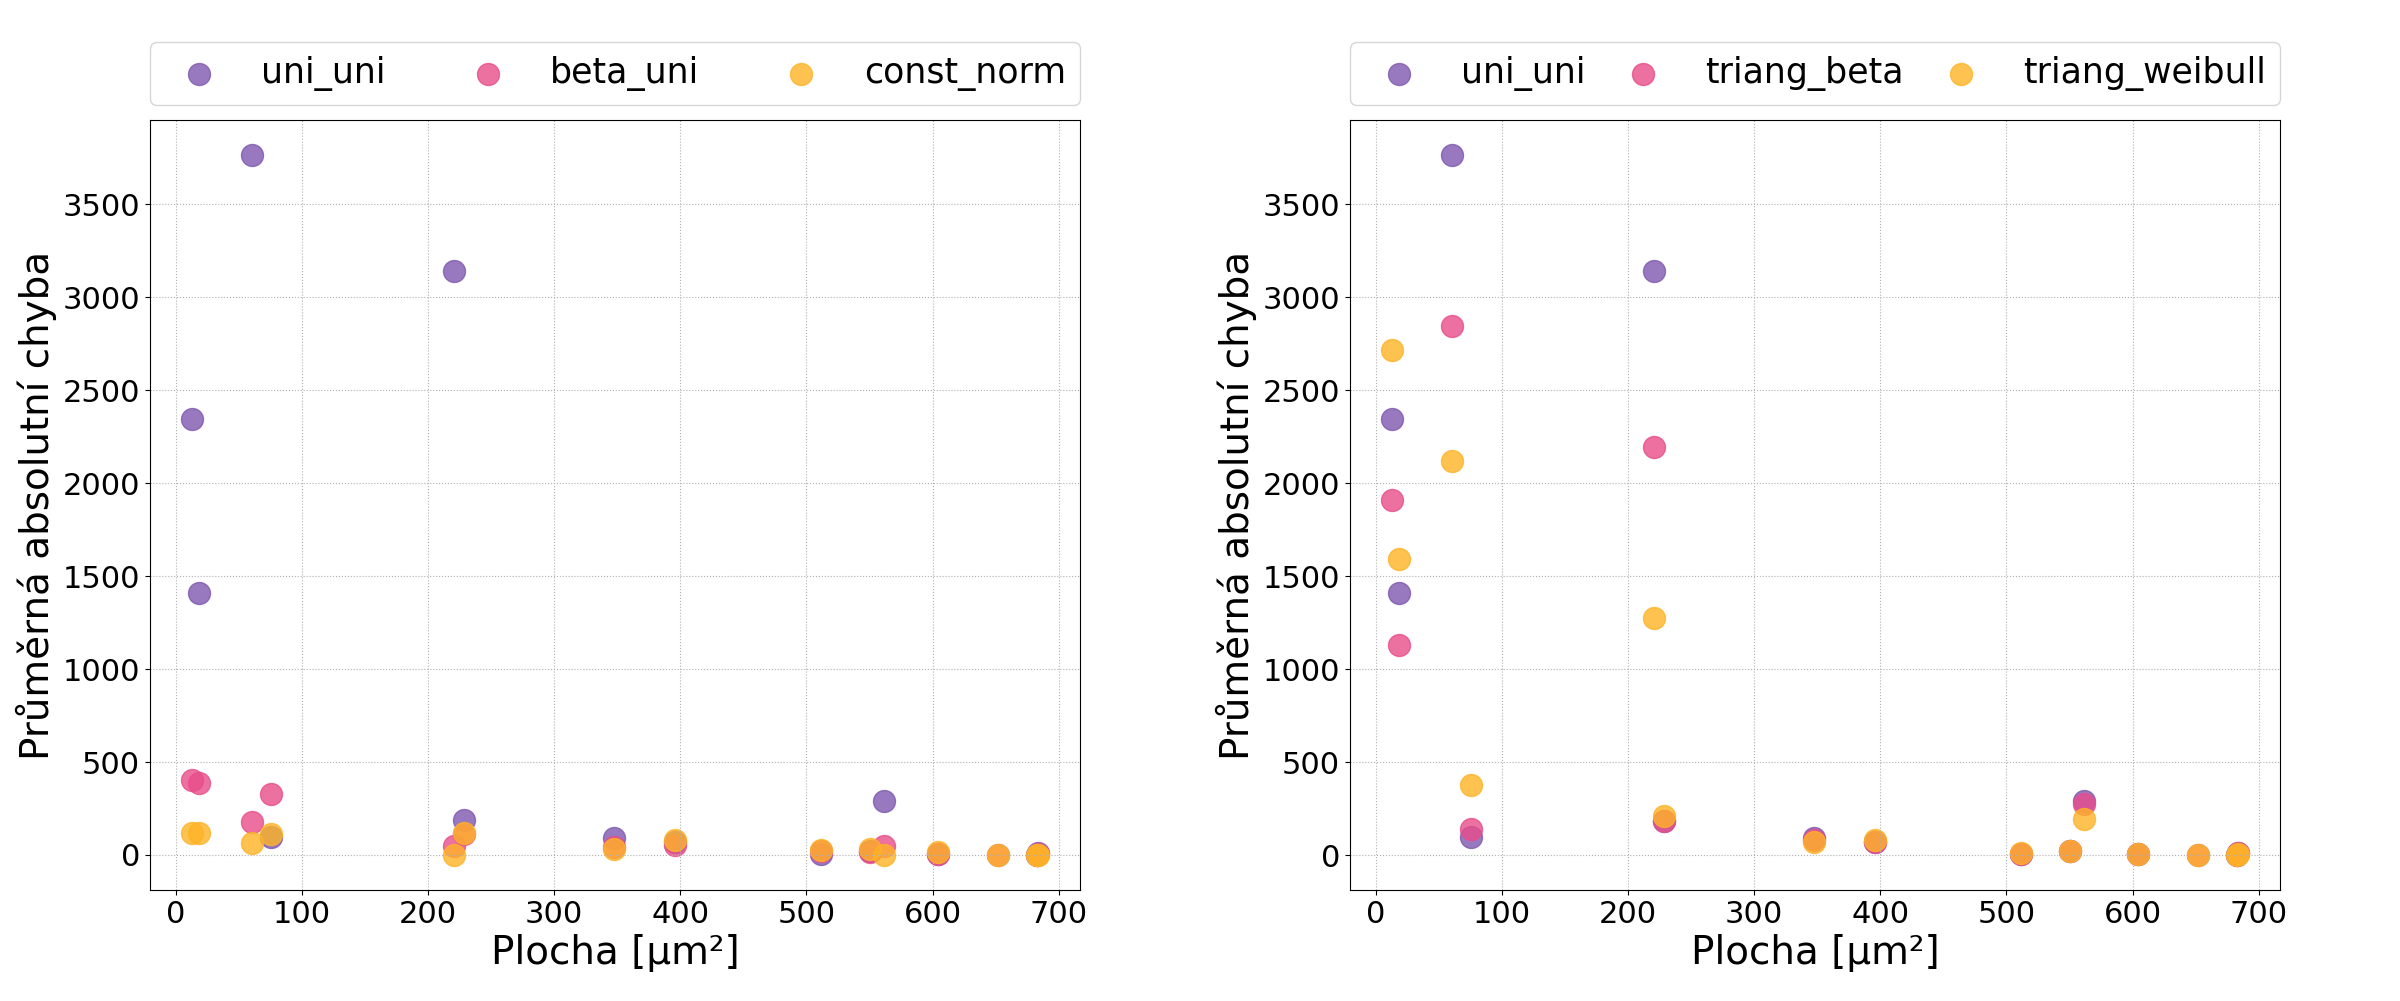
\includegraphics[width=\textwidth]{obrazky-figures/scatter_mean_abs_error.png}
    \caption{Porovnání průměrné absolutní chyby sledovaných násobiček v rámci vybraných rozdělení}
    \label{fig:scatter_mean_abs_error}
\end{figure}

\begin{figure}[H]
    \centering
    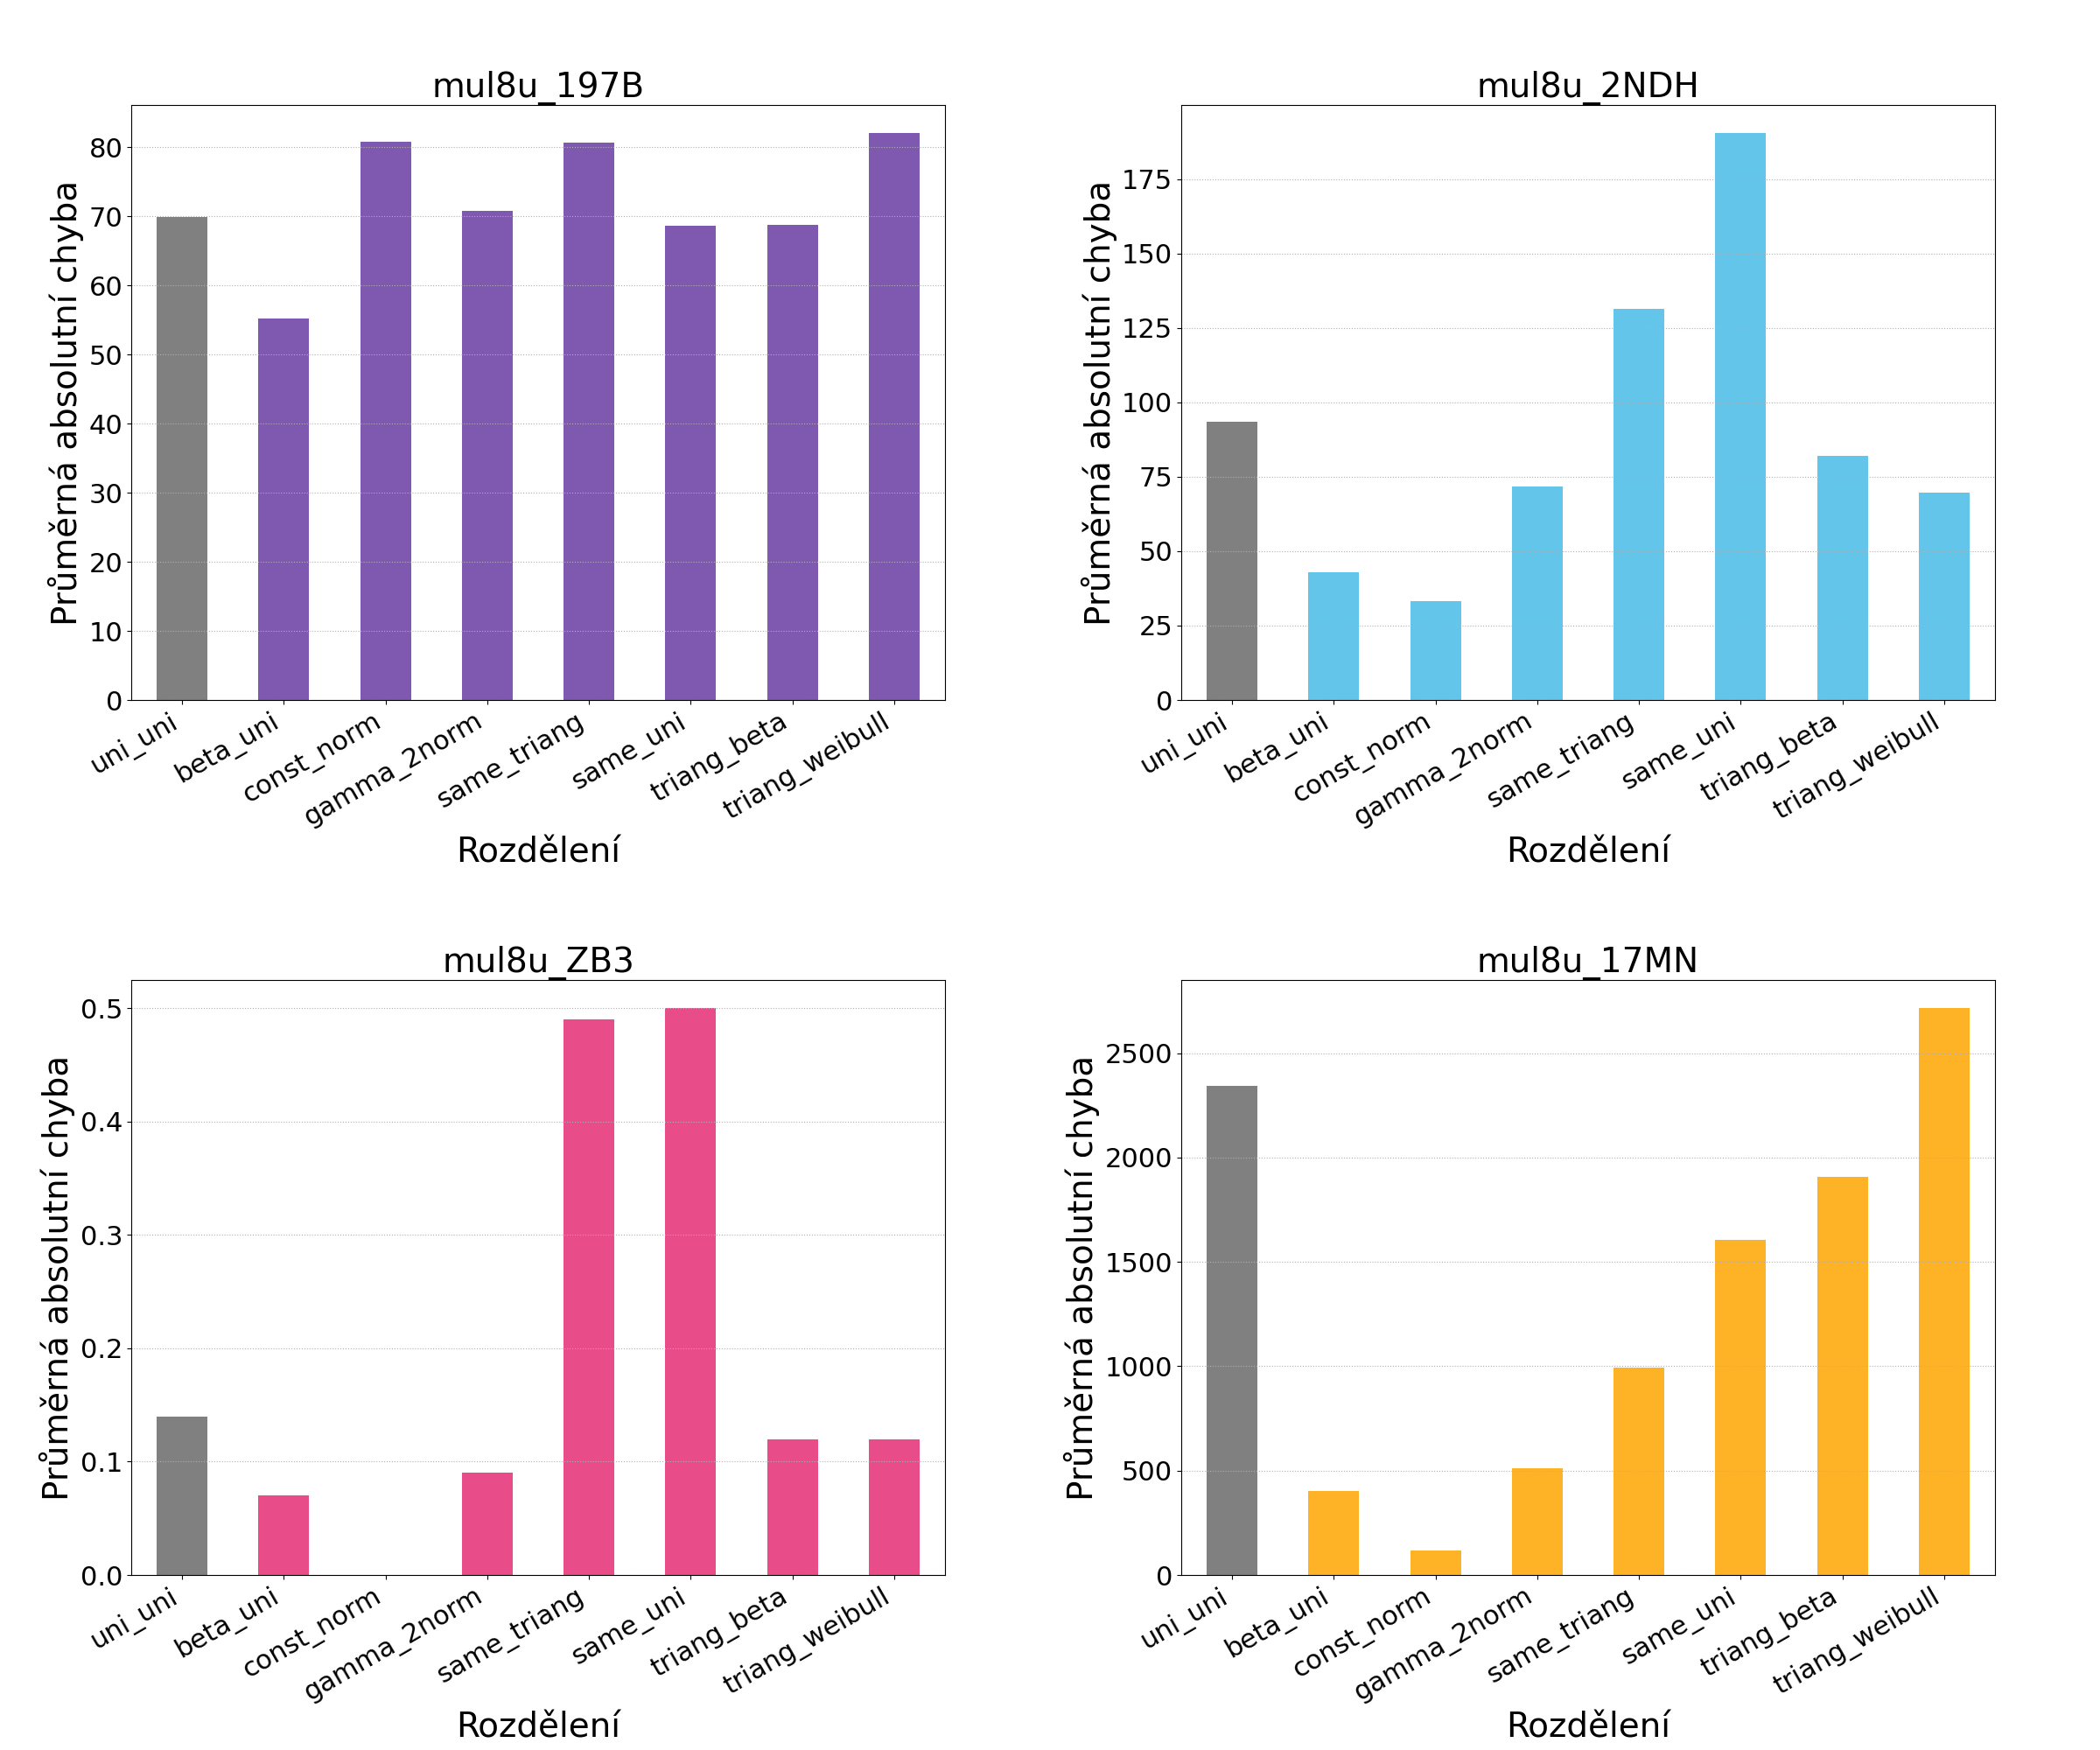
\includegraphics[width=\textwidth]{obrazky-figures/metrics_mean_abs_error.png}
    \caption{Průměrná absolutní chyba vybraných násobiček pro jednotlivá pravděpodobnostní rozdělení vstupních hodnot}
    \label{fig:metrics_mean_abs_error}
\end{figure}

\textbf{Průměrná relativní chyba} udává, jak velká chyba vznikla v porovnání s očekávaným výsledkem. Pokud měl například výsledek výpočtu být 3000 a výstup přibližného obvodu byl 2000, pak je relativní chyba $1/3$. 
V rámci výsledků simulací se větší relativní chyba vyskytovala u rozdělení, která generovala menší vstupy. To není překvapivé, neboť u malých výsledků se každá odchylka projeví ve výpočtu relativní chyby více, než je tomu u větších výsledků. Příklady relativní chyby vybraných násobiček lze pozorovat na obrázku \ref{fig:metrics_mean_relative_error}. Na obrázku \ref{fig:scatter_mean_relative_error} je vidět porovnání průměrné relativní chyby jednotlivých násobiček v rámci vybraných pravděpodobnostních rozdělení.

\begin{figure}[H]
    \centering
    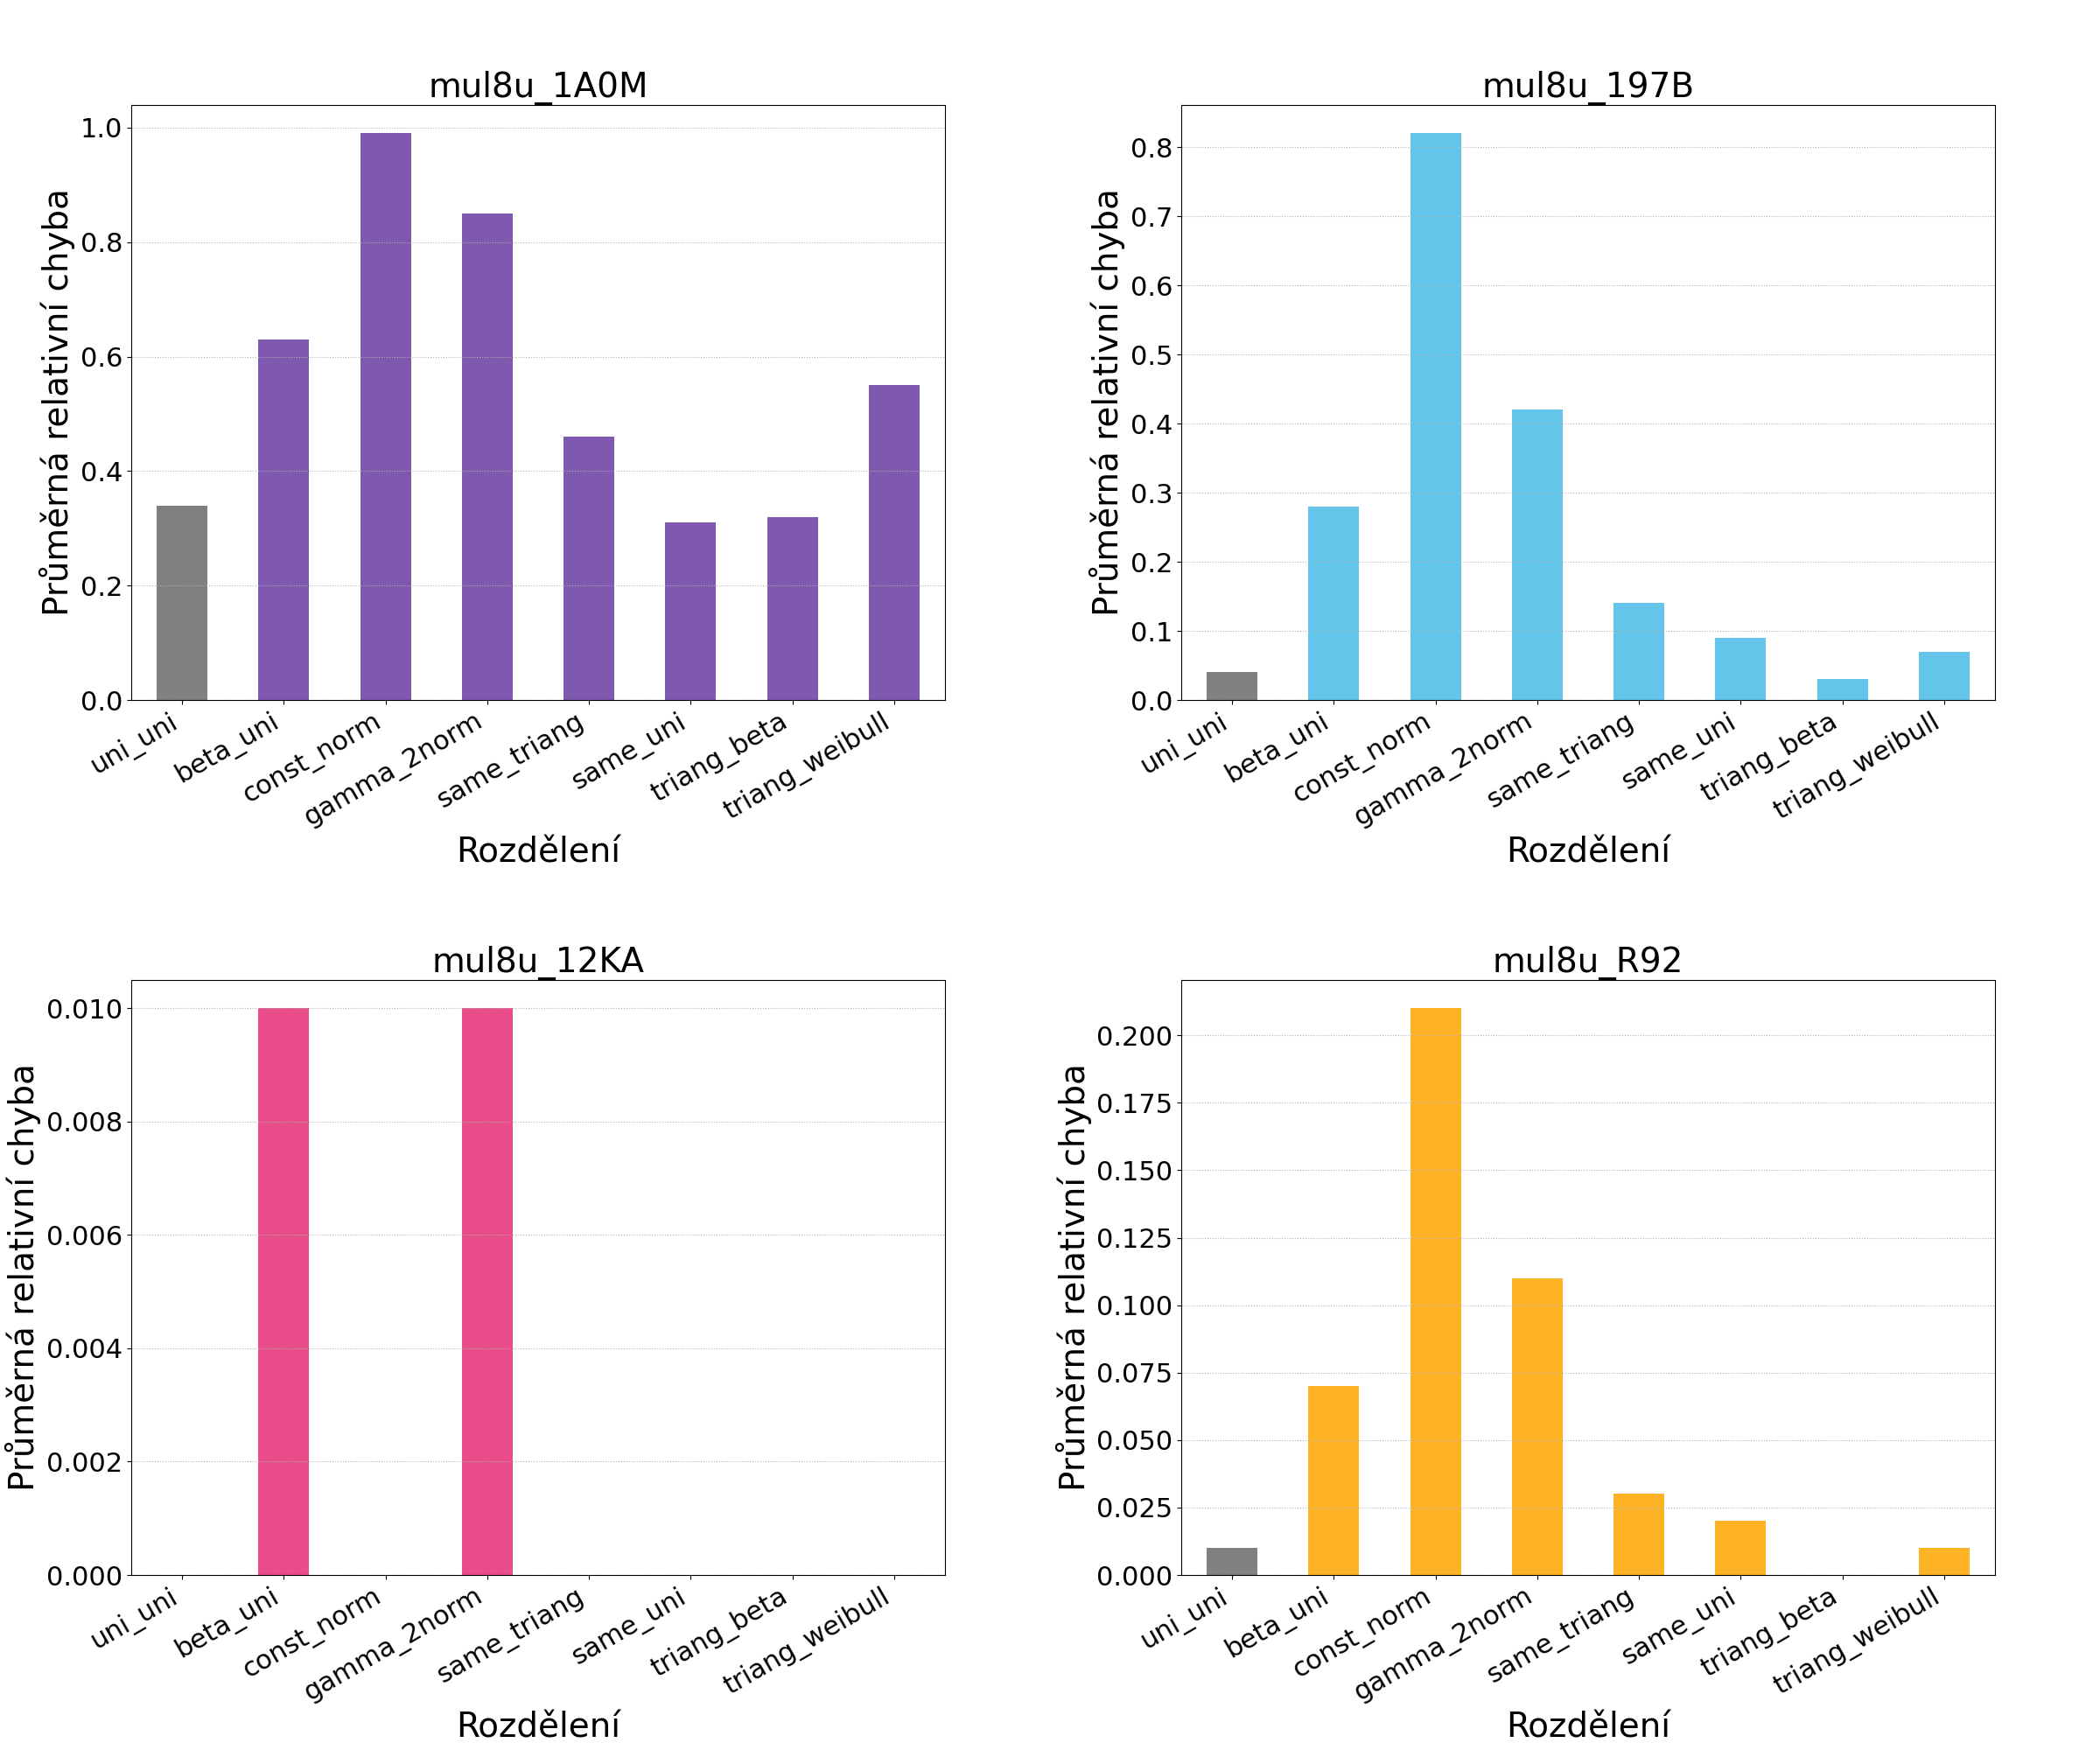
\includegraphics[width=\textwidth]{obrazky-figures/metrics_mean_relative_error.png}
    \caption{Průměrná relativní chyba vybraných násobiček pro jednotlivá pravděpodobnostní rozdělení vstupních hodnot}
    \label{fig:metrics_mean_relative_error}
\end{figure}

\begin{figure}[H]
    \centering
    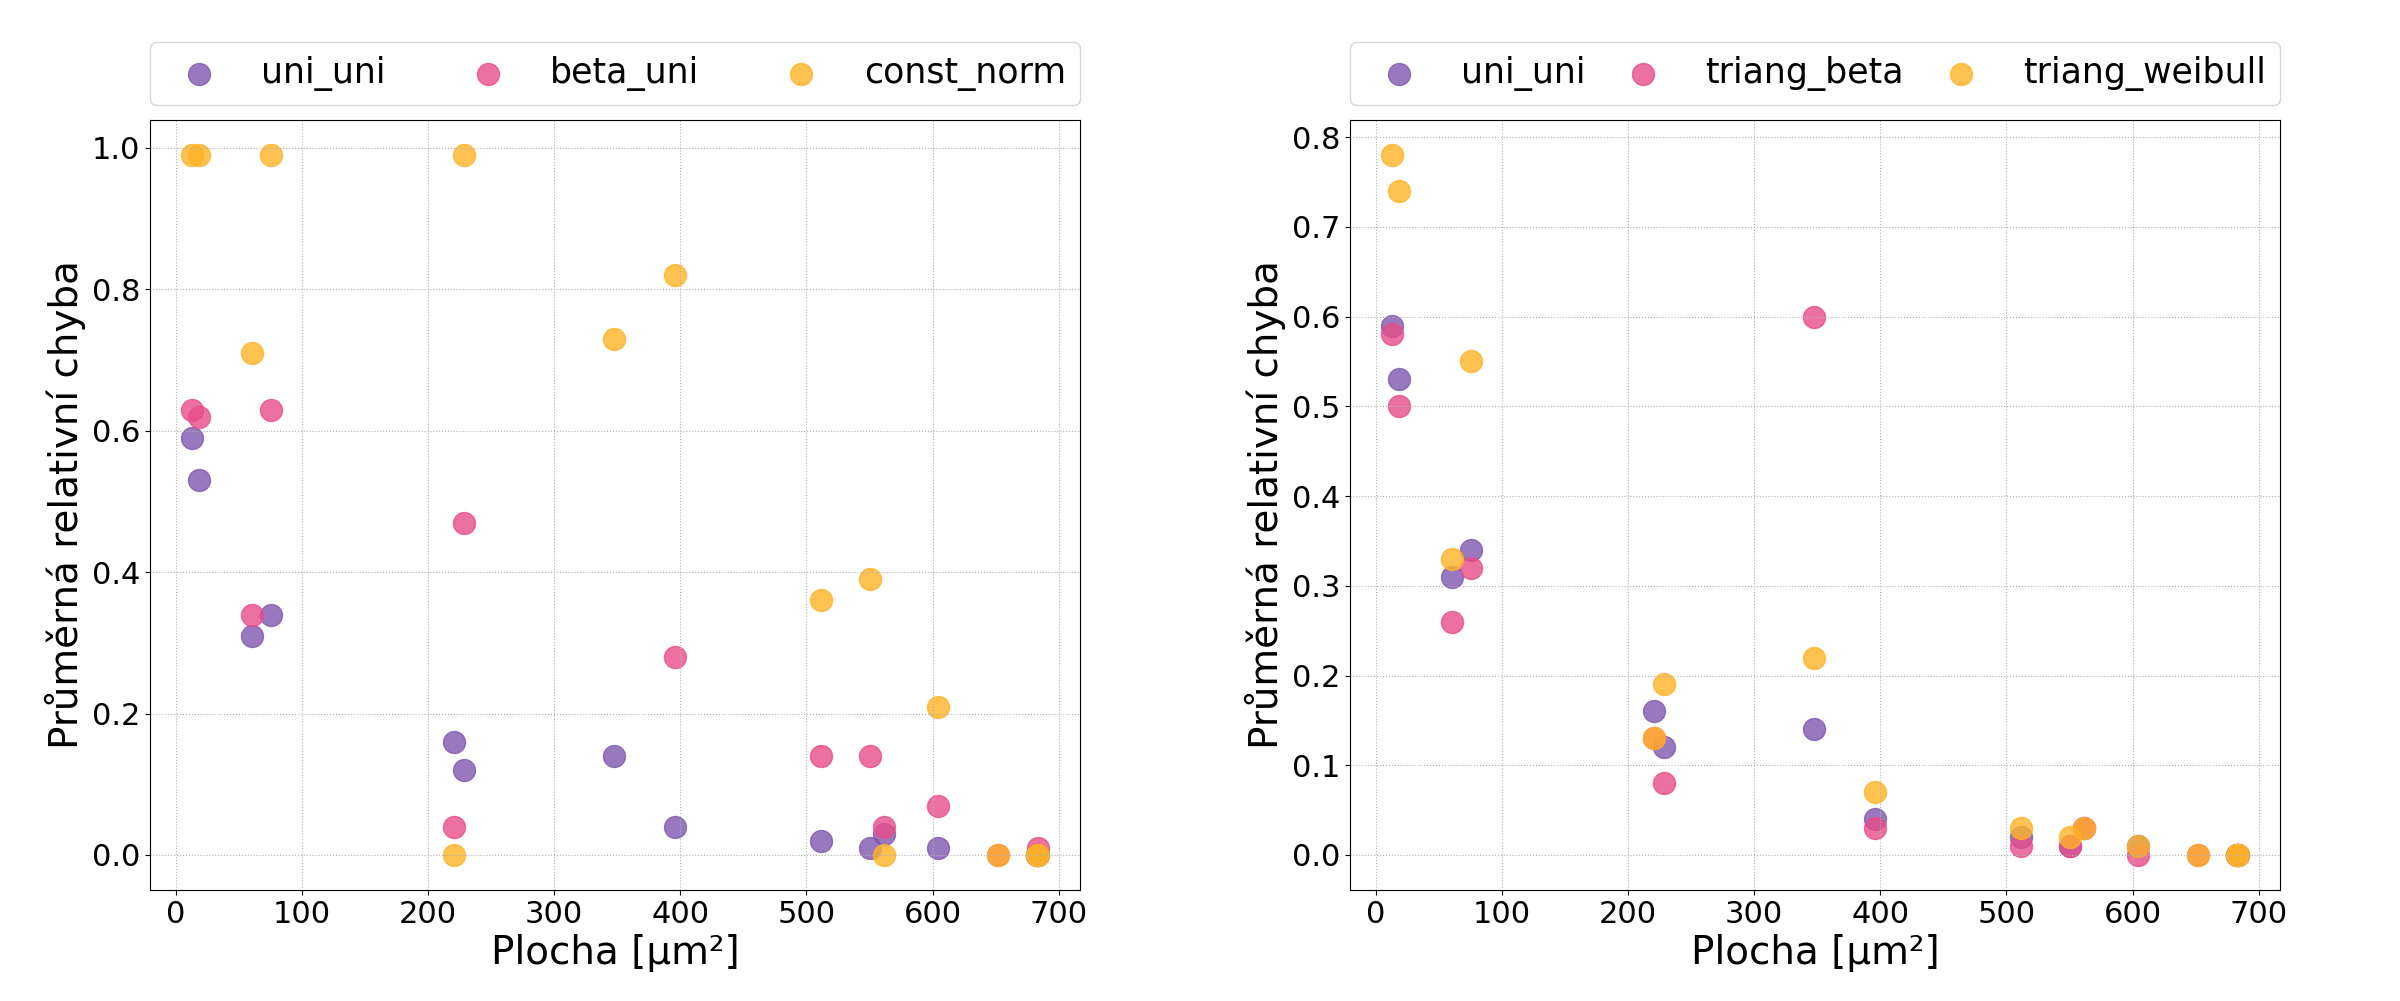
\includegraphics[width=\textwidth]{obrazky-figures/scatter_mean_relative_error.png}
    \caption{Porovnání průměrné relativní chyby sledovaných násobiček v rámci vybraných rozdělení}
    \label{fig:scatter_mean_relative_error}
\end{figure}

\textbf{Nejhorší absolutní chyba} bývala zpravidla nižší u rozdělení s menšími vstupy, potažmo výstupy. Míra tohoto typu chyby by nikdy neměla přesáhnout míru chyby naměřené při generování vstupů s referenčním rozdělením \texttt{uni\_uni}, neboť u tohoto rozdělení by v ideálním případě došlo k vygenerování všech vstupních kombinací. Při simulacích z časových úspor nedochází ke 100\% pokrytí všech vstupních kombinací, proto se občas může u jiného rozdělení vyskytnout mírně větší nejhorší absolutní chyba.

\begin{figure}[H]
    \centering
    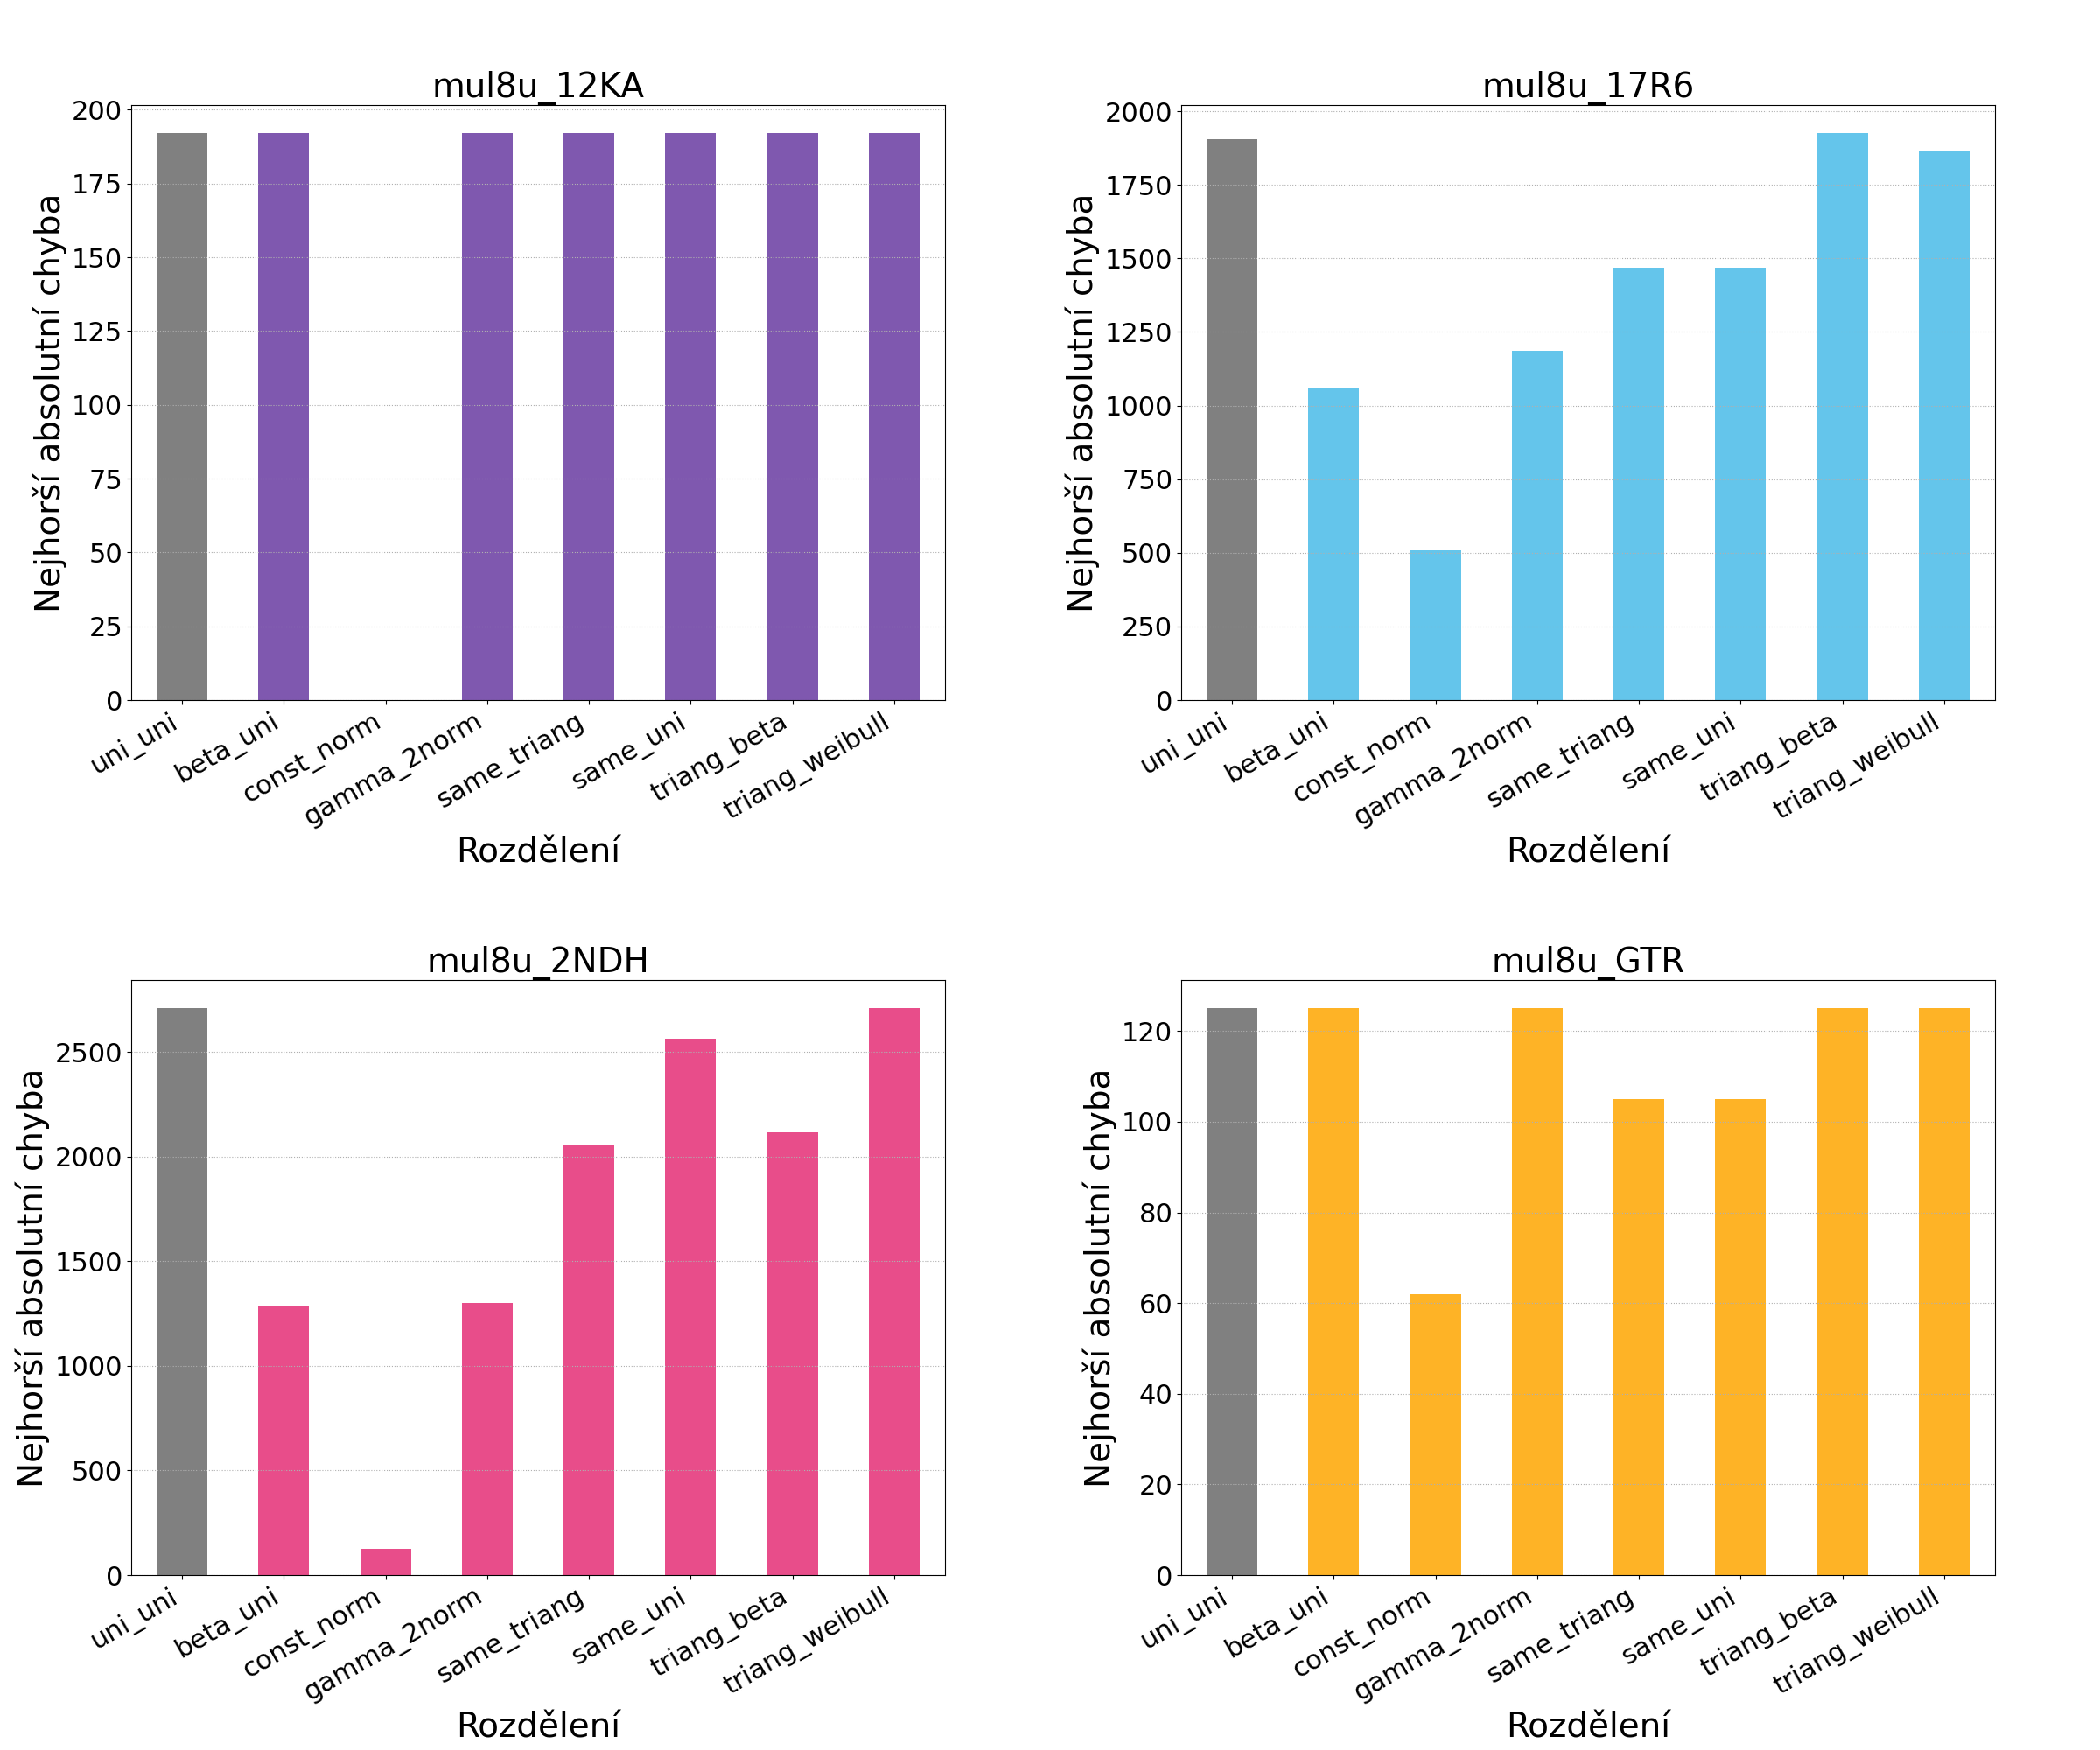
\includegraphics[width=\textwidth]{obrazky-figures/metrics_worst_case_error.png}
    \caption{Nejhorší absolutní chyba vybraných násobiček pro jednotlivá pravděpodobnostní rozdělení vstupních hodnot}
    \label{fig:metrics_worst_case_error}
\end{figure}

\chapter{Diskuze škálovatelnosti} 
\label{skalovatelnost}
Tato kapitola se zabývá škálovatelností modelovaného systému s ohledem na paměťovou a časovou náročnost. Simulace byly prováděny na počítači s následujícími parametry:
\begin{itemize}
    \item OS: Fedora Linux 39 (Workstation Edition),
    \item procesor: Intel Core i5-13600KF,
    \item paměť: 32 GB,
    \item verze software: UPPAAL 5.0.
\end{itemize}
Program UPPAAL se při simulacích nacházel v následujícím nastavení:
\begin{itemize}
    \item Search Order: Breadth First,
    \item Exploration: Exhaustive (Symbolic),
    \item State Space Reduction: Conservative,
    \item State Space Representation: Compact Data Structure,
    \item Diagnostic Trace: None,
    \item Back-propagation Order: Depth First,
    \item Search Priority: Automatic,
    \item Strategy: Entire winning strategy over all states,
    \item Extrapolation: Automatic,
    \item Hash Table Size: 16 MB,
    \item Learning Filter: Local Filter,
    \item Learning Method: Q-learning.
\end{itemize}
\pagebreak
V tabulce \ref{tab:scalability} jsou uvedeny výsledky měření pro vybrané násobičky. Násobičky z knihovny EvoApproxLib byly vybrány s ohledem na různý počet vstupních bitů a také na různý počet logických hradel. 

\begin{table}[!ht]
    \centering
    \begin{tabular}{|l|l|l|l|l|}
        \textbf{Násobička} & \textbf{Vstupní bity} & \textbf{Paměť [GB]} & \textbf{Čas [s]} & \textbf{Počet hradel} \\ \hline
        mul2u & 2x2 & 0.3 & 1 & 5 \\ 
        mul7u\_09Y & 7x7 & 3.7 & 75 & 73 \\ 
        mul7u\_073 & 7x7 & 4.3 & 760 & 154 \\ 
        mul7u\_01Q & 7x7 & 4.3 & 670 & 209 \\ 
        mul8u\_17MN & 8x8 & 8.9 & 85 & 10 \\ 
        mul8u\_R36 & 8x8 & 8.9 & 50 & 30 \\ 
        mul8u\_17R6 & 8x8 & 8.9 & 255 & 88 \\ 
        mul8u\_197B & 8x8 & 8.9 & 550 & 175 \\ 
        mul8u\_GTR & 8x8 & 8.9 & 1005 & 241 \\ 
        mul8u\_12KA & 8x8 & 8.9 & 1540 & 319 \\ 
    \end{tabular}
    \caption{Výsledky měření časové a paměťové náročnosti}
    \label{tab:scalability}
\end{table}

Jak je z výsledků patrné, paměťová náročnost závisí převážně na počtu vstupních bitů násobičky. Z toho důvodu bylo možné vyrobit násobičky s jinými vstupními bity, než jaké jsou k dispozici v knihovně EvoApproxLib. Toho bylo docíleno úpravou vybraných násobiček z knihovny -- odebráním přebytečných vstupních a výstupních bitů a signálů s nimi spojených. Na těchto násobičkách bylo poté opět provedeno měření s ohledem pouze na paměťovou složitost.

Výsledky lze pozorovat v tabulce \ref{tab:scalability_memory} a na obrázku \ref{fig:scalability_memory}. Dochází zde k exponenciálnímu růstu pravděpodobně z toho důvodu, že program UPPAAL při ověřování systému prochází velkou část stavového prostoru (ne nutně celý stavový prostor), který se s každým zvětšením násobičky o 2 výstupní bity zvětšuje čtyřikrát. Na násobičku 10x10 bitů již paměť referenčního stroje nestačila, proto lze pouze konstatovat, že paměťová náročnost této násobičky je větší než 32 GB.

\begin{figure}[H]
  \begin{minipage}[b]{.47\linewidth}
    \centering
    \begin{tabular}{|l|l|}
        \textbf{Vstupní bity} & \textbf{Paměť [GB]} \\ \hline
        2x2 & 0.3 \\ 
        3x3 & 0.4 \\ 
        4x4 & 0.42 \\ 
        5x5 & 0.44 \\ 
        6x6 & 1.1 \\ 
        7x7 & 3.7 \\ 
        8x8 & 8.9 \\ 
        9x9 & 24.8 \\ 
        10x10 & >32 \\ 
    \end{tabular}
    \captionof{table}{Paměťová náročnost dle počtu vstupních bitů}
    \label{tab:scalability_memory}
  \end{minipage}
  \begin{minipage}[b]{.47\linewidth}
    \centering
    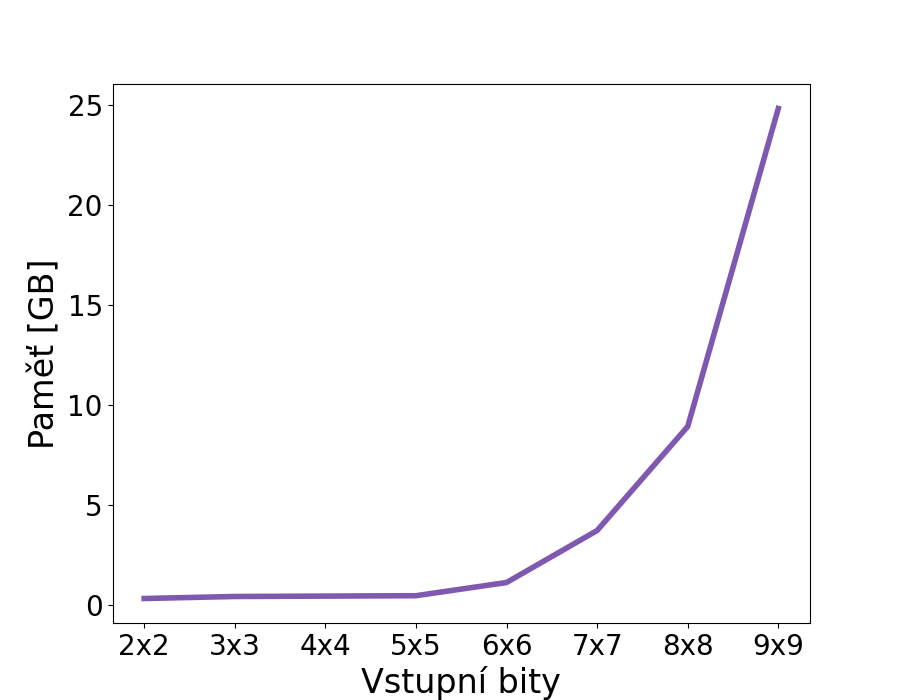
\includegraphics[width=\linewidth]{obrazky-figures/scalability_memory.png}
    \caption{Paměťová náročnost dle počtu vstupních bitů}
    \label{fig:scalability_memory}
  \end{minipage}\hfill
\end{figure}
\pagebreak
Časová náročnost simulací je lineárně závislá na počtu logických hradel v násobičce. Dále se časová náročnost odvíjí od výkonu procesoru počítače, na kterém jsou simulace prováděny. Na obrázku \ref{fig:scalability_time} je vidět časová náročnost v závislosti na počtu hradel u násobiček 7x7 a 8x8 bitů. Z grafu také plyne, že počet vstupních bitů násobičky nemá na časovou složitost simulace výrazný vliv. TODO možná víc dat, když bude čas.

\begin{figure}[H]
    \centering
    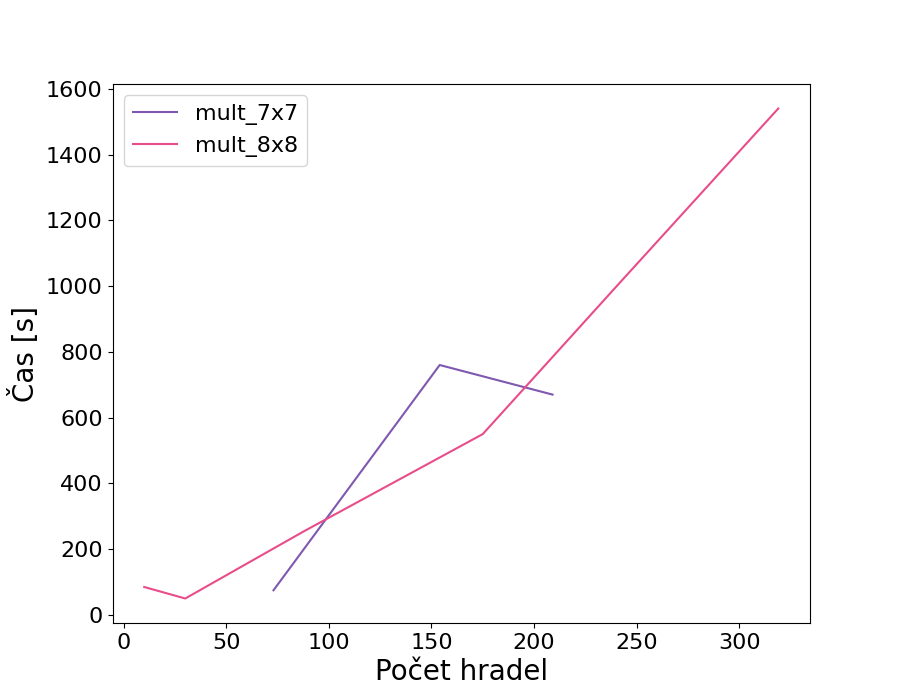
\includegraphics[width=0.8\textwidth]{obrazky-figures/scalability_time.png}
    \caption{Časová náročnost simulací v závislosti na počtu logických hradel}
    \label{fig:scalability_time}
\end{figure}

\chapter{Závěr}
\label{zaver}
TODO

%===============================================================================

% Pro kompilaci po částech (viz projekt.tex) nutno odkomentovat
%\end{document}

